\documentclass[11pt,a4paper,twoside]{book}
\usepackage{fontenc}[T1]
\usepackage[utf8]{inputenc}
\usepackage[english]{babel}
\usepackage{amssymb,amsmath}
\usepackage[top=2cm,bottom=2cm,left=2cm,right=2cm]{geometry}
\usepackage[pdftex]{graphicx} %per poter inserire le figure
\usepackage{amssymb,amsmath,amsthm,amsfonts}
\usepackage{xspace}
\usepackage{tabularx}
\usepackage{indentfirst}
\usepackage{subfigure}
\usepackage[small]{caption}
\usepackage{eucal}
\usepackage{eso-pic}
\usepackage{url}
\usepackage{booktabs}
\usepackage{afterpage}
\usepackage{parskip}
\usepackage{listings}
\usepackage{fancyhdr}
\usepackage{textcomp}
\usepackage{cite}
\usepackage{multirow}
\usepackage[utf8]{inputenc}   %per riuscire a scrivere gli accenti
\usepackage{setspace}
\usepackage{fancyhdr}
\newenvironment{abstract}{\cleardoublepage\thispagestyle{empty}\null\vfill\begin{center}\bfseries\abstractname\end{center}}{\vfill\null}
\pagestyle{fancy} 


\begin{document}
	\frontmatter
	\begin{titlepage}
		\vspace{5mm}
		\begin{figure}[hbtp]
			\centering
			
\includegraphics[scale=.16]{Logo_unipd.png}
		\end{figure}
		\vspace{5mm}
		\begin{center}
			{{\huge{\textsc{\bf UNIVERSIT\`A DEGLI STUDI DI PADOVA}}}\\}
			\vspace{5mm}
			{\Large{\bf Dipartimento di Fisica e Astronomia ``Galileo Galilei''}} \\
			\vspace{5mm}
			{\Large{\textsc{\bf Master Degree in Physics}}}\\
			\vspace{20mm}
			{\Large{\textsc{\bf Final Dissertation}}}\\
			\vspace{30mm}
			\begin{spacing}{3}
				{\LARGE \textbf{Proibing the Reheating Phase After Inflation}}\\
			\end{spacing}
			\vspace{8mm}
		\end{center}
		
		\vspace{20mm}
		\begin{spacing}{2}
			\begin{tabular}{ l  c  c c c  cc c c c c  l }
				{\Large{\bf Thesis supervisor}} &&&&&&&&&&& {\Large{\bf Candidate}}\\
				{\Large{\bf Prof. Nicola Bartolo}} &&&&&&&&&&& {\Large{\bf Raffaele Giusti}}\\
				{\Large{\bf Thesis co-supervisor}}\\
				{\Large{\bf Prof. Daniele Bertacca}}\\
			\end{tabular}
		\end{spacing}
		\vspace{15 mm}
		
		\begin{center}
			{\Large{\bf Academic Year 2021/2022}}
		\end{center}
	\end{titlepage}
	\clearpage{\pagestyle{empty}\cleardoublepage}

\begin{abstract}
	Inflation is the standard scenario, completely consistent with a variety of data, to understand the  
	generation of primordial scalar (density) perturbations, i.e.  the seeds of all the cosmological structures we  
	see today, and also of tensor perturbations (i.e. primordial gravitational waves). Inflation must come to an  
	end, in order for the universe to be filled in with radiation, and to proceed  through the standard radiation  
	dominated era, during which, e.g. primordial nucleosynthesis can take place. Such a transition (called  
	reheating phase) from the inflationary stage to the standard radiation dominated epoch, is the least known  
	part of the inflationary scenario, because, e.g., it involves couplings of the fields driving inflation to other  
	(relativistic) particles.  
	
	Nonetheless the precision of cosmological data has allowed recently to put already some constraints on  
	such a reheating phase.  
	
	This Thesis will provide an up-to-date review of all the cosmological observables that can be used to open  
	a new window into such period of the early universe. \\
	Moreover, we will also review the main models present in the literature about the preheating epoch (the initial stage of reheating) and the subsequent phases of reheating. These stages involve very non-linear and interesting physics and can lead to the production of gravitational waves that can be observed today.
\end{abstract}
	
\tableofcontents
	

\chapter{Introduction}

In modern cosmology one of the most important theories is represented by \textit{Cosmological Inflation}. \\
Inflation was an era during the early hystory of the Universe, before the epoch of primordial nucleosynthesis, during which the Universe expansion was accelerated. Such a period can be attained if the energy density of the Universe is dominated by the vacuum energy density associated with the potential of a scalar field, called the \textit{inflaton field} $ \phi $. \\
Inflation leads to a very rapid expansion of the Universe and can elegantly solve the flatness, the horizon and the monopole problems of the Standard Big Bang Cosmology (indeed, the first model of inflation by Guth in 1981 was introduced to address such problems \cite{Guth:Intro}). It can explain the production of the first density perturbations in the early Universe which are the seeds for the Large Scale Structure (LSS) in the distribution of galaxies and underlying dark matter, and for the Cosmic Microwave Background (CMB) temperature anisotropies that we observe today. Inflation has become the dominant paradigm to understand the initial conditions for structure formation and CMB anisotropies.\\
During this era primordial density fluctuations and gravitational waves are created from quantum fluctuations \textquotedblleft redshifted" out of the horizon during the rapid expansion and here \textquotedblleft frozen\textquotedblright.\\
From this period we can observe temperature anisotropy in the CMB caused by perturbations at the surface of the last scattering. The CMB temperature anisotropies are first detected by the Cosmic Background Explorer (COBE) satellite \cite{COBE1:intro},\cite{COBE2:intro}. \\
Another impressive confirmation of the inflationary theory has been provided by the data of the Wilkinson Microwave Anisotropy Probe (WMAP) mission that has produced a full-sky map of the angular variations of the CMB with unprecedented accuracy. WMAP data confirm the inflationary mechanism as responsible for the generation of superhorizon fluctuations \cite{WMAP:intro}, \cite{NonGauss:Intro}.\\
More recently, the best constraints on the CMB data are provided by the \textit{2018 Planck measurements} \cite{Planck2018:intro}. The \textit{Planck} data have given a very precise characteritation of the primordial cosmological perturbations and have allowed cosmological parameters to be constrained at the sub-percent level. Thus, \textit{Planck} measurements provide  a powerful constraint to inflationary models.\\

The literature contains a large number of different models of inflation. Each model amounts to a choice for the potential  of the inflaton, plus a period of ending inflation, called \textit{Reheating}.\\
The main models of inflation focuse on two different paradigms. Throughout the early 1990s discussion was dominated by the \textit{single-field models}. In these models, the scalar field potential often is chosen to be some convenient simple function, such as a monomial or exponential, and the initial conditions are chosen such that the scalar field is well displaced from any minimun.\\
In the mid-1990s, this paradigm was challenged by a new wave of inflationary model building, based on particle physics motivation such as the theories of supersymmetry, supergravity, and superstrings. In such a period we have a new class of models, known generically as \textit{hybrid inflation}, which rely on interactions between two scalar fields and utilize the flat potentials expected in supersymmetry theories \cite{Liddle:intro}. \\
In other scenarios we have the presence of a further scalar field besides the inflation that does not influence the inflationary dynamics (for example the \textit{curvaton scenario}), or the inflaton coupled to a scalar field or a gauge field. Finally, there are theories based on Modified Gravity (MG) that involve a modification of General Relativity \cite{GWFromInflation:Intro}.\\

Inflation cannot proceed forever. In fact, the greatest successes of the Standard Big Bang model, such as primordial nucleosynthesis and the origin of the CMB, require the standard evolution from radiation to matter dominated era.\\ 
The transition from inflation to later stages of the evolution of the Universe (radiation and matter dominance) is referred to as \textit{Reheating}. In the simplest models (single-field, slow-roll scenario) inflation ends when the inflaton field starts rolling fast along its potential, it reaches the minimun and then oscilates around it. During reheating the inflaton loses its energy, eventually leading the production of ordinary matter.\\
 More intricate scenarios include non perturbative processes such as (broad) resonance decay, tachyonic instability, instant preheating, fermionic preheating. The \textit{preheating} denotes the initial stage of reheating where we have an exponentially decay that generate high occupation numbers in selected frequency bands.  \\ 
 The aim of this Thesis is provide a complete and up-to-date review of the main models of reheating in the literature.
However, the reheating era is difficult to constrain observationally. In the absence of topological defects like monopoles or strings, the fluctuations produced during reheating remain sub-horizon and cannot leave an observable imprint at the level of the CMB or LSS. A lower bound is placed on the reheating temperature (\textit{i.e}. the temperature at which the standard radiation era of the Universe begins after reheating) by primordial nucleosynthesis (BBN) $ T_{BBN} \sim  10^{-2} Gev $ \cite{Steigman:nucleosynthesisIntro}. The scale of inflation is bounded from above and can be as large as $ \sim 10^{16} Gev $, leaving for the reheating temperature an allowed range of many orders of magnitude. 
Moreover, a variety of signatures relative to production of primordial black holes, magnetic field, unwanted relics, and also to mechanisms such as baryo - and leptogenesis, may be traced back to specific preheating/reheating models \cite{ReheatingPredictionsSingleFieldModel:intro} .\\ 

An extremely important prediction of cosmological inflation is the generation of a Stochastic Background of primordial Gravitational Waves (SGWB). Primordial GW are in fact not expected in the non inflationary standard early universe models and will provide, if detected, a \textit{smoking gun} probe of inflation. In the standard slow roll inflationary scenario tensor fluctuations of the metric (\textit{i.e} primordial GW) are characterized by a nearly scale invariant spectrum on super-horizon scales. The amplitude of the GW signal is usually described by the tensor-to-scalar ratio \textit{r}, defined as the ratio between the tensor and scalar power spectrum amplitudes at a given pivot scale $ k_{*} $.\\
The current best bound on $ \textit{r} $ comes from the joint analysis of Planck, BICEP2, Keck Array and other data, which yields $ r < 0.07 $ at $ 95 \% $ C.L. for $ k_{*}$ = $ 0.05\ Mpc^{-1} $ \cite{Bicep2:Intro}. \\
A crucial point is that, even in the simplest single field framework, different inflationary scenarios predict different values of r. The study of observational signatures of primordial GW thus provide not only a way to probe the general inflationary theory, but also to discriminate in detail among specific models.\\
A detection of primordial GW would not only be extremely important for Cosmology but also for High Energy and Fundamental Physics. Since the energy scale of inflation is directly linked to the value of the tensor-to-scalar ratio, by means of a detection of $ r $ we would obtain a hint of the the physics beyond the Standard Model and the precise indication of the energy regime of such new physics.\\
Indeed, the primordial GW are the object of a growing experimental effort, and their detection will be a major goal for Cosmology in the forthcoming  decades. \\
The main observational signature of the inflationary GW background is a curl-like pattern (B-mode) in the CMB. A number of, present or forthcoming, ground-based or baloon-borne experiments, are specifically aimed to B-mode detection. Unfortunately, the B-modes measured by BICEP2 \cite{Bicep2BMode:Intro} did not point to any inflationary signal, but several next-generation CMB space missions have been proposed in recent years with the specific goal of B-mode detection such as COrE \cite{COre:intro} or PRISM \cite{PRISM:intro}. 
Finally, we have the possibility of a future direct detection, by experiments such as aLIGO \cite{LIGO:intro}, or eLISA \cite{Lisa:Intro}, especially if some inflationary models produced a blue-tilted primordial tensor spectrum \cite{GWFromInflation:Intro}.\\
In this thesis we will focus on another type of GW: those generated by classical mechanism during reheating after inflation. By investigating  GW we cannot neglect this stage. In fact, there are many models for the reheating period which provide further GW production, besides that inflationary stage. Moreover, it can be shown that reheating parameters are related to inflationary power-spectra ones, so that the constraints on tensor perturbations are related to those on the reheating period.


In this work we are going to review all the most important inflation and reheating scenarios. After the first two chapters, we will present detailed models of reheating about each of its stages (Preheating, Bubbly Stage, Scalar Wave Turbolence, Thermalitation) investigated in the literature. Moreover, we will review predictions about the production of GW, observable signatures on CMB and the possibility of direct detection of GW from reheating epoch.\\
The Thesis is organized with the following plan:\\
In the chapter 1 we review the standard single-field model of slow-roll inflation and we derive the physical observables that can be seen and constrained from CMB. \\
In chapter 2 we overview the main inflationary models that are important for the subsequent reheating epoch and a simple model of reheating is presented.\\ In chapter 3 we explain more deeply how gravitational waves are generated during inflation and reheating, and how they can put some constraints about the reheating epoch. Moreover, we derive some quantities important for such stage coming from CMB observables.\\
In the chapter 4, we investigate about \textit{Preheating}, the first stage of reheating, in the model of parametric resonance. \\
In  chapter 5 we examinate the other important model of preheating: preheating after hybrid inflation. Then, we briefly consider other models of preheating such as fermionic preheating, instant preheating and multi-field reheating.\\
In  chapter 6 and 7 we examinate the subsequent and final stages after preheating: the bubbly stage and thermalitation.\\
In chapter 8 we present the results found in the literature about the gravitational waves generated during the reheating stage on basis of the models presented.\\
In chapter 9 we  overview the principal signatures  of the reheating epoch.
 
 \mainmatter
 
\chapter{Inflation}

The inflation theory not only provides an excellent way to solve flatness and horizon problems but also generates density perturbations as seeds for large-scale structure in the universe. Quantum fluctuations of the field that drives inflation (called \textit{inflaton}) are streched on large scales by the accelerated expansion. In the simplest version of the single-field scenario the fluctuations are \textquotedblleft frozen" after the scale of perturbations leaves the Hubble radius during inflation. Long after the inflation ends, the perturbations cross inside the Hubble radius again. Thus, inflation provides a causal mechanism for the origin of large-scale structure in the universe. An important prediction of inflation is that density perturbations generally exhibit nearly scale-invariant spectra. This prediction can be directly tested by the measurement of the temperature anisotropies in Cosmic Microwave Background (CMB). Indeed, the anisotropies observed by the Cosmic Background Explorer (COBE) in 1992 showed nearly scale invariant spectra. All data acquired until now have continued to confirm the main predictions of the inflationary theory within observational errors \cite{InflationDynamicsAndReheating:chap1}.\\
In this first chapter we review the simple standard model of slow-roll inflation and we derive observables and relations that will be used in the next chapters.

\section{Standard Big-Bang Cosmology}

The standard big-bang cosmology is based upon the cosmological principle which requires that the universe is homogeneous and isotropic on averaging over large volumes.\\
A homogeneous and isotropic universe is described by the Friedmann-Robertson-Walker metric (FRW):

\begin{equation}
	\label{metric}	
	ds^{2}   = - dt^{2} + a^{2}(t)\Big[\frac{dr^{2}}{1-Kr^{2}}  +  r^{2}(d\theta^{2} + sin^{2} \theta d\phi^{2})\Big] . 
\end{equation}
Here $a(t)$ is the scale factor with $ t $ being the cosmic time and $(r,\theta,\phi) $ are comoving (spherical) coordinates. The constant $ K $ is the spatial curvature, where positive, zero, and negative values correspond to closed, flat, and hyperbolic spatial sections respectevely. \\
The evolution of the universe is dependent on the material within it. A key role is played by the \textit{equation of state} relating the energy density $ \rho (t) $ and the pressure $ P(t) $. Assuming a perfect and barotropic fluid we can describe it with the relation $ P=\omega\rho $ with $ \omega=0 $ for non-relativistic matter (dust) and $ \omega=1/3 $ for radiation.
For example in the universe we have $ P=0 $ or $ P=1/3 $ if it is dominated by dust or radiation, respectevely. \\
The dynamical evolution of the universe is known once we solve the Einstein equations for General Relativity:

\begin{equation}
	\label{eq:gr}
	G_{\mu\nu}  = R_{\mu\nu} - \frac{1}{2}g_{\mu\nu}R=8\pi G T_{\mu\nu}
\end{equation}

where $ G_{\mu\nu} $ is the Einstein Tensor, $ R_{\mu\nu} $, $ R $, $ T_{\mu\nu}$, and G are the Ricci tensor, Ricci scalar, energy-momentum tensor and gravitational constant, respectively. The energy momentum tensor $ T_{\mu\nu} $ describes the perfect fluid with density energy $ \rho $ and isotropic pressure P that fills the universe.\\
The Planck energy, $M_{pl}=1.2211 \times 10^{19}$ GeV, is related to G through the relation $ M_{pl} = (\hslash c^{5}/G)^{1/2}$. Hereafter we use the units $ \hslash = c = 1 $.\\
From the Einstein equations (\ref{eq:gr}) for the background FRW metric (\ref{metric}), we obtain the Friedmann Equations:
\begin{equation}
	\label{friedmannEquations1}
	H^{2}=\frac{8\pi G}{3}\rho - \frac{K}{a^{2}},
\end{equation}
\begin{equation}
	\label{friedmannEquations2}	
	\frac{\ddot{a}}{a} = -\frac{4\pi G}{3}(\rho + 3P),
\end{equation}

where the dots denote the derivative with respect to t, and $ H=\dot{a}/a $ is the Hubble expansion rate. Combining these relations we obtain the energy conservation equation 

\begin{equation}
	\label{energyCons}
	\dot{\rho} + 3H(\rho + P)=0,
\end{equation}

which is known as the continuity or fluid equation.\\
The Friedmann equation (\ref{friedmannEquations1}) can be rewritten as 

\begin{equation}
	\label{densityParameter}
	\Omega - 1 = \frac{K}{a^{2}H^{2}}
\end{equation}

where 

\begin{equation}
	\label{criticalDensity}
	\Omega=\frac{\rho}{\rho_{c}}, \quad    with \quad   \rho_{c}=\frac{3H^{2}}{8\pi G}
\end{equation}

where the density parameter $ \Omega $ is the ratio of the energy density to the critical density $ \rho_{c} $.\\
When the spatial geometry is flat (K=0, $ \Omega $=1) the solution for equations (\ref{friedmannEquations1})
and (\ref{friedmannEquations2}) are $ a \propto t^{1/2} \quad  (\rho \propto a^{-4}) $ for the radiation dominated era, and $ a\propto t^{2/3} \quad  (  \rho \propto  a^{-3}$) for dust dominated era.\\
Thus, from these equations we obtain a decelerate expansion ($ \ddot{a} < 0 $) for the universe.\\

\section{Standard cosmology and inflation}
In this section we briefly review the problems with the standard cosmology and how are solved by the idea of inflation \cite{Liddle:intro},\cite{Dodelson:Chap1}, \cite{InflationDynamicsAndReheating:chap1}. 

\subsection*{\emph{Flatness problem}}
In the standard big-bang theory with $ \ddot{a} < 0  $, the $ a^{2}H^{2} (= \dot{a}^{2}) $ term in (\ref{densityParameter}) always deacreases. This means that
$ \Omega $ tends to evolve away from unity with the expansion of the universe. Howewer, since present observations suggest that $ \Omega  $ is within a few percent of unity today, $ \Omega $ is forced to be much closer to unity in the past. For example, we require $ |\Omega-1| < \mathcal{O}(10^{-16}) $ at the epoch of nucleosynthesis and  $ |\Omega-1| < \mathcal{O}(10^{-64}) $ at the Planck epoch \cite{Liddle:intro}. This appears an extreme and innatural fine-tuning of initial conditions. Unless initial conditions are chosen  very accurately, the universe either collapses too soon, or expands too quickly before the structure can be formed. This is the so-called \textit{flatness problem}.

\subsection*{\emph{Horizon problem}}
Consider a comoving wavelength, $ \lambda $, and the corresponding physical wavelength, $ a\lambda $, which at some time is inside the Hubble radius, $ H^{-1} $ (\emph{i.e. a$ \lambda \leq  H^{-1}  $}). The standard big-bang cosmology is characterized by the cosmic evolution of  $a \propto t^{n} $ with 0 $< n < 1$. In this case the physical wavelength grows as $ a\lambda \propto t^{n} $, whereas the Hubble radius evolves as $H^{-1}\propto t$ . Therefore the physical wavelength becomes much smaller than the Hubble radius at late times.
This means that a causally connected region can only be a small fraction of the Hubble radius.\\
For example if we observe photons in the cosmic microwave background (CMB) which are last-scattered at the time of decoupling turns out that the causally connected regions on the surface of last scattering corresponds to an angle of order 1°.\\
This appears to be in contrast with observations of the CMB which has the same temperature to high precision in all directions on the sky. There is no way to establish thermal equilibrium if these points were never been in causal contact before last scattering. This is the so-called \textit{horizon problem} .

\subsection*{\emph{Large-scale structure}}
Experiments which observe temperature anisotropies in the CMB find that the amplitude of the anisotopies is small and their power spectrum is close to scale-invariant on large scales. It is impossible to generate such fluctuations  via causal processes in a FRW metric in the time between the big bang and the time of the last scattering.

\subsection*{\emph{Relic density problem}}
In Particle Physics the standard paradigm to study the fundamental interactions is the Spontaneous Symmetry Breaking (SSB) of gauge symmetries.\\
In the early universe the breaking of such symmetries leads to the production of many unwanted relics such as monopoles, cosmic strings, and other topological defects \cite{TopDefects:Linde}. For example, any grand unified theory based on a simple Lie group that includes the U(1) of electromagnetism must produce monopoles. String theories also predict supersymmetric particles such as gravitinos, Kaluza-Klein particles, and moduli fields.\\
If these massive particles exist in the early stages of the universe and they are stable (or sufficiently long-lived) could become the dominant matter in the early universe depending on their number density and therefore contradict a variety of observation such as those of the light element abundances. This problem is known as the \textit{relic density problem}.

\subsection*{\emph{The idea of inflation}}

The problems in the standard big bang cosmology lie in the fact that the universe always exhibits decelerated expansion. Instead, let us assume  the existence of a stage in the early universe with an accelerated expansion: 

\begin{equation}
	\label{acc.expansion}
		\ddot{a} > 0
\end{equation}

From the relation (\ref{friedmannEquations2}) this gives the condition

\begin{equation}
	\label{equationOfState}
	\rho + 3P < 0
\end{equation}

and, from  the equation of state $ P = \omega \rho  $, we obtain 

\begin{equation}
	\label{w parameter}
	\omega < -\frac{1}{3}
\end{equation}

The condition (\ref{acc.expansion}) essentialy means that $ \dot{a}\ (= aH) $ increases during inflation and hence that the comoving Hubble radius, $ (aH)^{-1} $, decreases in the inflationary phase.

\subsubsection*{\textit{Flatness problem}}
Since the $ a^{2}H^{2} $ term in (\ref{densityParameter}) increases during inflation, $ \Omega $ is rapidly driven towards unity. After the inflationary period ends, the evolution of the universe is followed by the conventional big-bang phase and $|\Omega-1| $ begins to increase again. As long as the inflationary expansion lasts sufficiently long and drives $ \Omega $ very close to one, $ \Omega $  will remain close to unity even in the present epoch.  

\subsubsection*{\textit{Horizon problem}}
Since the scale factor evolves approximately as $ a \propto t^{n} $ with n $ > 1 $ during inflation, the physical wavelength, $a \lambda $, grows faster than the Hubble radius, $ H^{-1}(\propto t)$. Therefore, physical wavelenghts are pushed outside the Hubble radius during inflation and then causally connected regions can be much larger than the Hubble radius, thus potentially solving the horizon problem.\\
A detailed computation shows this is achieved when the universe expands at least about $ e^{70} $ times during inflation, or 70 e-folds of expansion \cite{Liddle:intro}.

\subsubsection*{\textit{Large-scale structure}}
The inflationary period leads to perturbations of the scalar field that drives inflation and then of the energy density of the universe. In the early stage of inflation the scales of these perturbations are well within the Hubble radius and causal physics can works generating small quantum fluctuations. During the later stages these scales are pushed outside the Hubble radius (\textit{i.e.} the first Hubble radius crossing). Fluctuations of the scalar field become over-damped on long-wavelengths and the perturbations can be described as classical on these large scales. After the inflationary period these scales of perturbations  cross inside the Hubble radius again (\textit{i.e.} the second Hubble radius crosssing).\\
The small perturbations imprinted during inflation have amplitudes determined by the Hubble rate which is approximatevely constant during this period and hence  leads to an almost scale-invariant spectrum with constant amplitude on different scales.\\
In this way the inflation naturally provides a causal mechanism to generate the seeds of density perturbations observed in the CMB anisotropies.

\subsubsection*{\textit{Relic density problem}}
During the inflationary phase the energy density of massive particles scales as $ a^{-3} $, much faster than the energy density  of the universe (considering $ a \propto t^{n} $ with $ n>1 $, we have $ H \propto t^{-1} \propto a^{-1/n}$ that leads $  \rho \propto a^{-2/n} $). Thus, these particles are red-shifted away during inflation, solving the monopole problem.

\section{The inflaton equation}
As we have seen  from (\ref{w parameter}) a period of inflation is possible if the pressure $ P $ is negative with 

\begin{equation}
\label{Pressure-density}
P < -\frac{\rho}{3}
\end{equation}

In the special case in which $ \omega = -1 $ ($P=-\rho$) we have a period in the hystory of the universe called \textit{de Sitter stage}. \\
Such a period can be obtained inserting a cosmological constant $ \Lambda $ in the Einstein Equations: 

\begin{equation}
	\label{RGModified}
	R_{\mu\nu} - \frac{1}{2}g_{\mu\nu}R = 8\pi G T_{\mu\nu} - \Lambda g_{\mu\nu}.
\end{equation}

Considering the energy continuity equation (\ref{energyCons}) and the first Friedmann equation (\ref{friedmannEquations1}) we see that in a de Sitter phase $ \rho = constant $ and $ H = H_{inf} \simeq constant $ (we neglect the curvature K which is soon redshifted away as $ a^{-2} $).\\
Solving the second Friedmann equation (\ref{friedmannEquations2}) we obtain an exponentially growing of the scale factor

\begin{equation}
	\label{scaleFactorDeSitter}
	a(t)=a_{i} e^{ H_{inf}(t-t_{i})}	
\end{equation}

where $t_{i}$ is the time at which inflation starts. \\
The cosmological constant can be interpreted as the energy of the quantum vacuum state of the system, the \textit{vacuum} energy density contributed by any particle species. Even if it is simple to have such exponentially expansion of the universe the inflation must end at some point. Thus, there must be some dynamics regulating such system.\\
We can obtain this if we consider a scalar field, called the \textit{inflaton}, that dominates the energy in this epoch and leads the expansion.\\

Consider in full generality the total action

\begin{equation}
	\label{totalAction}
	S^{TOT} = S_{HE} + S_{\phi} + S_{m} 
		        = \frac{1}{16\pi G} \int d^{4} x \sqrt{-g} (R + \mathcal{L} [\phi , \partial_{\mu} \phi ] + \mathcal{L}_{matter}) 	
\end{equation}

where $ g $ is the determinant of the metric tensor $ g_{\mu\nu} $, $ S_{HE} $ is the Hilbert-Einstein action, $ S_{\phi} $ is the inflaton scalar field action and $ S_{m} $ is the action of the rest of the matter besides the inflaton (fermions, gauge fields, other scalars...). We will neglect $ S_{m} $ because, in general, they are subdominant at early times. \\
The action for a minimally-coupled real scalar field $ \phi $ is given by

\begin{equation}
	\label{actionScalarField}
	S=\int d^{4} x \sqrt{-g} \mathcal{L} = \Big [-\dfrac{1}{2} g^{\mu\nu} \partial_{\mu}\phi \partial_{\nu} \phi - V(\phi)\Big]	
\end{equation}

where $ V(\phi) $ specifies the scalar field potential and  can have different forms depending on the model. For example it can be a simple quadratic potential $ V(\phi)=\frac{1}{2}m^{2}\phi^{2} $, with $ m $ the mass of the particle associated to $ \phi $,$  $ or can describes  self interactions $ V(\phi) = \frac{\lambda}{4} \phi^{4} $. $ V(\phi) $ can represent also interactions of $ \phi $ with other fields and contains quantum radiative corrections. \\

To characterize the evolution of the scalar field in an expanding universe we can associate to $ \phi $ its stress-energy momentum $ T_{\mu\nu} $, which in General Relativity is given from a generic lagrangian by

\begin{equation}
	\label{stressEnergyMomentum}
	T_{\mu\nu}= \frac{-2}{\sqrt{-g}}\frac{\delta S}{\delta g^{\mu\nu}}=
	\frac{-2}{\sqrt{-g}}\Big [-\frac{\partial (\sqrt{-g} \mathcal{L})}{\partial g^{\mu\nu}} + \partial _{\alpha} \frac{\partial (\sqrt{-g} \mathcal{L})}{\partial \partial_{\alpha} g^{\mu\nu}} + ... \Big ].
\end{equation}

Assuming a minimally-coupled field (\textit{i.e.} doesn't involve direct coupling with gravity, e.g. $ \varepsilon  \phi^{2} R$ terms), the stress-energy tensor assumes the form

\begin{equation}
	\label{tensorScalrField2}
	T^{\phi}_{\mu\nu} = -2 \frac{\partial \mathcal{L}_{\phi}}{\partial g^{\mu\nu}} + g^{\mu\nu} \mathcal{L}_{\phi}
 =\partial_{\mu} \phi \partial_{\nu} \phi + g_{\mu\nu} \Big [-\frac{1}{2}g^{\mu\nu}\partial_{\mu}\phi\partial_{\nu}\phi - V(\phi)\Big]
\end{equation}

The equation of motion for $ \phi $ is derived by varying the action (\ref{actionScalarField}) with respect $ \phi $ obtaining the Klein-Gordon equation

\begin{equation}
	\label{KGEquation}
	\square  \phi = \frac{\partial V}{\partial \phi}	
\end{equation}

where $\square$ is the covariant D'Alembert operator

\begin{equation}
	\label{alembertOperator}
	\square \phi = \frac{1}{\sqrt{-g}}\partial_{\nu}\Big (\sqrt{-g} g^{\mu\nu} \partial_{\mu}\phi\Big ).
\end{equation}

In a FRW universe described by the metric (\ref{metric}), the evolution equation for $ \phi $ becomes

\begin{equation}
	\label{eomForPhi}	
	\ddot{\phi} + 3H\dot{\phi} - \frac{\nabla^{2} \phi}{a^{2}} + V'(\phi)=0
\end{equation}

where $ V'(\phi)=dV/d\phi $. Through $ 3H\dot{\phi} $ the field "feels" a friction due to the expansion of the universe, which will play a crucial role.\\

We can now express the inflaton field $ \phi $ as the sum of the classical background value and the field fluctuations

\begin{equation}
	\label{splitInflaton}
	\phi(t,\textbf{x})=\phi_{0}(t) + \delta \phi(t,\textbf{x})
\end{equation}

where $\phi_{0}(t) =\ <0|\phi(t,\textbf{x})|0> $  is the classical field, that is the expectation value of the inflaton field on the initial isotropic and homogeneous state, while $\delta \phi (t,\textbf{x})$ represents the quantum fluctuations around $ \phi_{0}(t)$.
We will consider first the background dynamics and then the evolution of quantum perturbations during inflation. This separation is justified by the fact that quantum fluctuations are much smaller than the classical value and therefore negligible when looking at the classical evolution.

\section{Classical Dynamics}
The inflaton field $ \phi(t) $  behaves like a perfect flud with background energy density and pressure given by 

\begin{equation}
	\label{energyDensityPressure}
	T^{0}_{0} = -\Big [\dfrac{1}{2} \dot{\phi}^{2}_{0}(t) + V(\phi_{0}) \Big ] = -\rho_{\phi}(t)
\end{equation}
\begin{equation*}
	T^{i}_{j} = -\Big [\dfrac{1}{2} \dot{\phi}^{2}_{0}(t) - V(\phi_{0}) \Big ]\delta^{i}_{j} = \delta^{i}_{j} P_{\phi} (t)	
\end{equation*}

where $ \rho_{\phi} (t) $ is the energy density and $ P_{\phi} (t) $ the isotropic pressure. $ T_{\mu\nu} $ is diagonal and the spatial part is the same in every direction as a consequence of isotropy and homogeneity resulting in a tensor typical of perfect fluids. Hereafter we don't insert the subscript \textquotedblleft 0" when we denote the background field. \\
Therefore if 

\begin{equation}
	\label{conditionFlatPotential}
	V(\phi) \gg \frac{1}{2} \dot{\phi}^{2}
\end{equation}

we see that 

\begin{equation}
	\label{deSitterCondition}
	P_{\phi} \simeq -\rho_{\phi}
\end{equation}

which gives rise to a quasi-de-Sitter phase.\\
From this simple calculation we realize that a scalar field whose energy is dominant in the universe and whose potential energy dominates over the kinetic term gives inflation. The condition (\ref{conditionFlatPotential}) is called \textit{slow-roll} regime, during which $ V(\phi) \simeq constant $ provides accelerated expansion driven by the vacuum energy density of $ \phi $, which mimics an effective cosmological constant $ \Lambda $.\\
The ordinary matter fields, in the form of a radiation fluid, and the spatial curvature K are usually neglected during inflation because their contribution to the energy density is redshifted away during the accelerated expansion.
\begin{figure}
	\centering
	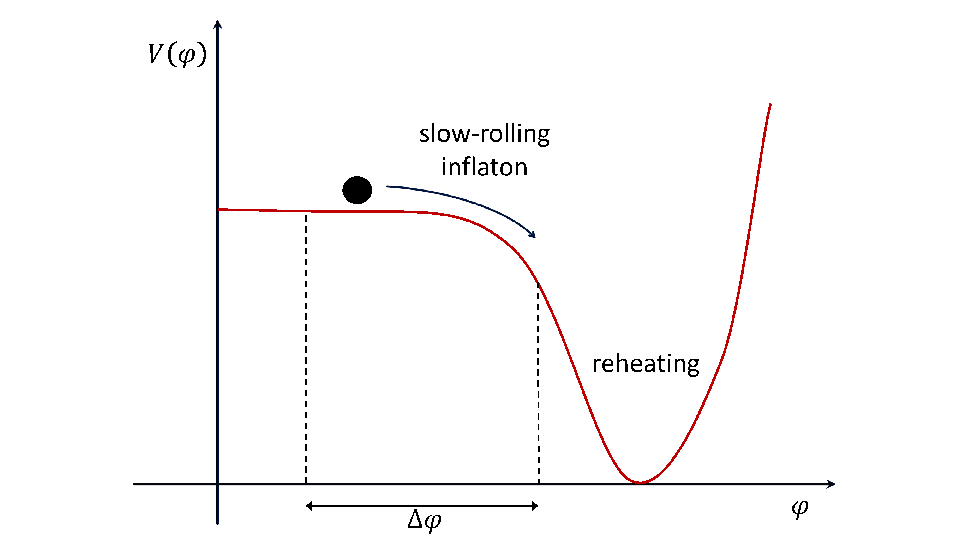
\includegraphics[width=0.65\linewidth, height=0.25\textheight]{Images/Chap1/GWFromInflation_Fig1}
	\caption{Example of inflationary potential with a flat region. After the slow-roll of the inflaton field $\phi$, the reheating phase starts. The field oscillates around the minimum of the potential and decays in other particles. $\Delta$ $\phi$ indicates the inflaton excursion between the horizon exit of a comoving scale and the end of inflation \cite{GWFromInflation:Intro}. }
	\label{fig:gwfrominflationfig1}
\end{figure}

\subsection{Slow-roll parameters}

We quantify now under which circumstances a scalar field may give rise to a period of inflation.
Considering the background scalar field $ \phi $ (homogeneous and isotropic) the equation of motion (\ref{eomForPhi}) becomes

\begin{equation}
	\label{eomHomogeneousField}
	\ddot{\phi} + 3H \dot{\phi} + V'(\phi) = 0.
\end{equation}

If the \textit{slow-roll} condition $ \phi^{2} \ll V(\phi) $ is satisfied, the scalar field slowly rolls down its potential. Such a period can be achieved if the inflaton field is in a region where the potential is sufficiently flat. Since the potential is flat we may also expect that $\ddot{\phi}$ is negligible as well. We will assume this is true and we will quantify this condition.\\
Requiring the slow-roll condition the Friedmann equation (\ref{friedmannEquations1}) becomes 

\begin{equation}
	\label{friedMannEqDuringInflation}
	H^{2} \simeq \frac{8\pi G}{3} V(\phi),
\end{equation}

where we assumed that the inflaton field dominates the energy density of the universe. Moreover, assuming also $\ddot{\phi}$ negligible we obtain the new equation of motion

\begin{equation}
	\label{newEQMphiDotDotNegligible}
	3H\dot{\phi} = -V'(\phi)
\end{equation}

Using (\ref{newEQMphiDotDotNegligible}) and the slow-roll condition (\ref{conditionFlatPotential}) we obtain

\begin{equation}
	\label{condition1}
	\frac{(V')^{2}}{V} \ll H^{2}
\end{equation}

and, considering $\ddot{\phi} \ll 3H\dot{\phi}$,

\begin{equation}
	\label{condition2}
V'' \ll H^{2}	.
\end{equation}

These two conditions represent the flatness conditions of the potential which are conveniently parametrized in terms of the so-called \textit{slow-roll parameters}.
The slow-roll parameters quantify the slow-roll regime dynamics in order to give predictions of specific models and to compare it with others and with observations.\\
Firstly, we define the $\epsilon$ parameter

\begin{equation}
	\label{epsilon}
	\epsilon = - \frac{\dot{H}}{H^{2}}
\end{equation}

that describes how much $ H $ changes during inflation.
To relate this variable to the slow-roll relation $ \dot{\phi}^{2} \ll V(\phi) $ let us derive the first Friedmann equation (neglecting the curvature)

\begin{equation}
	\label{derivingEpsilon1}
	H^{2}=\frac{8\pi G}{3}\rho_{\phi} = \frac{8\pi G}{3} \Big (\frac{1}{2}\dot{\phi}^{2} + V(\phi) \Big )
\end{equation}

obtaining,

\begin{equation}
	\label{FriedmannDerived}
	2H\dot{H} = \frac{8\pi G}{3} \Big (\dot{\phi} \ddot{\phi} + V'(\phi)\dot{\phi} \Big ).
\end{equation}
Now, inserting the equation of motion of the inflaton $ \ddot{\phi} = -3H\dot{\phi} - V'  $ in (\ref{FriedmannDerived}) we obtain

\begin{equation}
	\label{Hdot}
	\dot{H} = -4\pi G\dot{\phi}^{2}
\end{equation}

Finally, using $ H^{2}=(8\pi G/3)V(\phi) $  

\begin{equation}
	\label{epsilon2}
	\epsilon= - \frac{\dot{H}}{H^{2}}=4\pi G \frac{\dot{\phi}^{2}}{H^{2}} \simeq \frac{3}{2} \frac{\dot{\phi}^{2}}{V(\phi)}
\end{equation}

where the last equality si valid only in the slow-roll regime. Therefore, we can interpret $\epsilon$ as the ratio between the kinetic energy and the potential. \\
Hence assuming $ V(\phi) \gg \dot{\phi}^{2}  $ we obtain 

\begin{equation}
	\label{conditionEpsilon}
	\epsilon \ll 1 .
\end{equation}
Moreover, exploiting $ H\dot{\phi} \simeq -V' $, we can write

\begin{equation}
	\label{newEpsilon}
	\epsilon=4\pi G \frac{\dot{\phi}^{2}}{H^{2}} \simeq \frac{1}{16\pi G} \Big (\frac{V'}{V} \Big )^{2}	
\end{equation}

which means that if $\epsilon \ll 1 $ , $V'$ is small and the potential is flat. Thus, $\epsilon$ quantifies the flatness of the potential.\\

Considering the second slow-roll condition $ \ddot{\phi} \ll 3H\dot{\phi} $, we can define the second slow-roll parameter as 

\begin{equation}
	\label{etaParameter}
	\eta = - \frac{\ddot{\phi}}{H\dot{\phi}} \ll 1
\end{equation}

As we have done for $\epsilon$ we can relate this expression to the potential. To do this we can derive $ \dot{\phi} \simeq -V'/3H $, obtaining

\begin{equation}
	\label{phiDerivedEtaParameter}
	\ddot{\phi} = -\frac{V'' \dot{\phi}}{3H} + \frac{\dot{H}}{3H^{2}}V'.
\end{equation}
Plugging this into the definition of $\eta$ we obtain

\begin{equation}
	\label{eta2}
	\eta \simeq \frac{V''}{3H^{2}} - \frac{\dot{H}}{H^{2}}\frac{V'}{3H\dot{\phi}} \simeq \eta_{V} - \epsilon
\end{equation}

where $ \frac{V'}{3H\dot{\phi}} \simeq -1 $ and we have defined $ \eta_{V}=\frac{V''}{3H^{2}} $. Thus again, having $\eta \ll 1$ means to have a flat potential.\\

A successful period of inflation requires that $ \epsilon, |\eta| \ll 1 $. Moreover, exists a hierarchy of slow-roll parameters: for example, one can define the slow-roll parameter related to the third derivative of the potential

\begin{equation}
	\label{secondOrderParameter}
	\xi^{2} = \Big (\frac{1}{4\pi G} \Big )^{2} \Big (\frac{V'V'''}{V^{2}}\Big )
\end{equation}

which is a second order slow-roll parameter. The third derivative of the potential corresponds to an eventual self-interaction of the inflaton field. \\
One can use these parameters with the data collected from observations to reconstruct the shape of the potential.\\
At first-order in the slow-roll parameters $\epsilon$ and $\eta$ can be considered constant, since the potential is very flat and their derivatives are higher orders in these parameters. In fact it is easy to see that $ \dot{\epsilon},\dot{\eta} = \mathcal{O}(\epsilon^{2},\eta^{2}) $.\\

If we written $ \epsilon = - \dot{H}/H^{2} $ we can notice that

\begin{equation}
	\label{scaleFactorParameter}
	\ddot{a}=\dot{\dot{a}}=\dot{(aH)}=\dot{a}H + a\dot{H}=aH^{2}\Big (1+\frac{\dot{H}}{H^{2}}\Big ) = aH^{2}(1-\epsilon) .
\end{equation} 

Thus, inflation can be attained only if $\epsilon < 1$. As soon as this condition fails, inflation ends.\\
This condition alone can be sufficient to realise inflation. However, having also $\eta \ll 1 $  assure that inflation lasts for long enough. In fact, $ \eta = - \frac{\ddot{\phi}}{H\dot{\phi}}  \ll 1 $ both ensures that inflation is an attractor solution and that $\dot{\phi}$ remains constant and small for long enough. In other worlds, $\eta$ controls the duration of inflation.\\

Despite the semplicity of the inflationary theory, the number of inflationary models that have been proposed so far is enormous, differing for the kind of potential and for the underlying particle phyisics theory. In the second chapter we will discuss about the most important models, but we just to mention here that the main classification in connection with the observations is the one in which the single-field inflationary models are divided into three broad groups as \textquotedblleft small field", \textquotedblleft large field" (or chaotic) and \textquotedblleft hybrid" type, according to the region occupied in the ($\epsilon$ - $\eta$) space by a given inflationary potential.\\

\section{Inflation and cosmological perturbations}
The description of the universe as a perfectly homogeneous and isotropic FRW model is an idealitation. Actually, we are interested in deviations from homogeneity and isotropy that enable us to characterise different models.\\
So far we have considered only the dynamics of a homogenous scalar field driving inflation. But to investigate inflation models in more detail and to test theoretical predictions against cosmological observations we need to consider inhomogeneous perturbations. \\
Besides the background inflationary dynamics, we have the evolution of the quantum fluctuactions of the inflaton field $ \delta\phi(t,\textbf{x}) $. In the inflationary model there are primordial energy density perturbations, associated with these vacuum fluctuations, which survive after inflation and are the origin of all the structures in the universe.\\
Once the universe became matter dominated ($ z \simeq 3200 $) primeval density inhomogeneites ($ \delta \rho/\rho \simeq 10^{-5} $) were amplified by gravity and grew into the structure we see today. The existence of these inhomogeneities was in fact confirmed by the COBE discovery of CMB anisotropies.\\
In this section we summarise how the quantum fluctuations of a generic scalar field evolve during an inflationary stage. For more details see \cite{Liddle:intro},\cite{NonGauss:Intro},\cite{Dodelson:Chap1}.

\subsection{Quantum Fluctuations}
Consider for semplicity a scalar field $ \phi $ (the inflaton) with an effective potential $ V(\phi) $ in a pure de Sitter stage, during which the Hubble rate $ H $ is constant. 
We first split the field $ \phi(\tau,\textbf{x}) $ in the homogeoneous classical part, $ \phi(\tau) $, and its fluctuations $ \delta\phi(\tau,\textbf{x}) $

\begin{equation}
	\label{splitInflatonTau}
	\phi(\tau,\textbf{x})=\phi(\tau) + \delta \phi(\tau,\textbf{x})
\end{equation}

where $ \tau $ is the conformal time, related to the cosmic time $ t $ through $ d\tau=dt/a(t) $.\\
We consider the Fourier transform of the fluctuations
\begin{equation}
\label{fourierTransform}
\delta\phi(\tau,\textbf{x})=\frac{1}{(2\pi)^{3}}\int d^{3}k e^{i \textbf{k}\cdot\textbf{x}}\delta\phi(\tau,k).
\end{equation}
Redefining  the scalar field as 
\begin{equation}
\label{fieldRedefinition}
\widetilde{\delta \phi}	= a\delta\phi
\end{equation}
 we can promote it to an operator which can be decomposed as 
 \begin{equation}
 	\label{quantitation}
 	\widetilde{\delta \phi}(\tau,\textbf{x})=\int \frac{d^{3} \textbf{k}}{(2\pi)^{3/2}} \big[u_{k}(\tau)a_{\textbf{k}}e^{i \textbf{k}\cdot\textbf{x}} + u_{k}^{*}(\tau)a_{\textbf{k}}^{\dagger}e^{-i \textbf{k}\cdot\textbf{x}}\big]
 \end{equation}
 
 where we have introduced the creation and annihilation operators $ a_{\textbf{k}} $ and $ a^{\dagger}_{\textbf{k}} $.\\
 The creation and annihilation operators for $\widetilde{\phi}$ satisfy the standard commutation relations
 \begin{equation}
 	\label{commutationRelations}
 \big[a_{\textbf{k}},a_{\textbf{k}'}] = 0, \qquad \big[a_{\textbf{k}},a_{\textbf{k}'}^{\dagger}] = \delta^{(3)}(\textbf{k}-\textbf{k}')
 \end{equation}
and the modes $ u_{k}(\tau) $ are normalized so that they satisfy the condition

\begin{equation}
	\label{normalitation}
	u^{\ast}_{k} u_{k}' - u_{k} u'^{\ast}_{k} = -i,
\end{equation}
where primes denote derivatives with respect to the conformal time $ \tau $. \\
Expanding the equation of motion for the scalar field (\ref{eomForPhi}) in the fluctuations $\delta\phi(\tau,\textbf{x})$ in Fourier space we obtain
\begin{equation}
	\label{eomFluctuations}
	u''_{k}(\tau) + \Big[k^{2} - \frac{a''}{a} + \frac{\partial^{2} V}{\partial\phi^{2}}a^{2}\Big] u_{k}(\tau) = 0.
\end{equation}

 where $ m^{2}_{\phi} = \partial^{2} V / \partial\phi^{2} $ is the effective mass of the scalar field. This equation describes an harmonic oscillator with a frequency changing in time, due to the expansion of the universe.\\
 The modes $ u_{k}(\tau) $ at very short distances must reproduce the form for the ordinary flat space-time quantum field theory. Thus, well within the horizon, in the limit $ k/aH \rightarrow \infty $, the modes should approach plane waves of the form
 
 \begin{equation}
 	\label{planeWave}
 	u_{k}(\tau) \rightarrow \frac{1}{\sqrt{2k}}e^{-ik\tau}.
 \end{equation}

Let us consider a special case where the inflaton is massless in a pure de-Sitter universe ($m_{\phi} = 0, H=constant $). In this situation the equation (\ref{eomFluctuations}) becomes
\begin{equation}
\label{eomMasslessDesitter}
u''_{k}(\tau) + \Big[k^{2} - \frac{a''}{a}\Big]u_{k}(\tau) = 0.
\end{equation}

Using $a d\tau=dt$, and $ a \propto e^{Ht}$ in a de-Sitter stage 
\begin{equation}
	\label{horizon}
	\frac{a''}{a}= \frac{2}{\tau^{2}}=2a^{2}H^{2}=\frac{2}{r_{H}^{2}}
\end{equation}
where $ r_{H} $ is the comoving Hubble radius.\\
Thus, we can study (\ref{eomMasslessDesitter}) in two different regimes: the \textit{sub-horizon} regime where $ \lambda_{phys} \ll H^{-1} $, $ k^{2} \gg a^{2}H^{2} \simeq a''/a $, and the \textit{super-horizon} regime where $ \lambda_{phys} \gg H^{-1} $, $ k^{2} \ll a^{2}H^{2} \simeq a''/a $.\\
In the sub-horizon case the equation of motion reduces to the wave equation

\begin{equation}
\label{waveEquationFluctuation}
u''_{k} + k^{2}u_{k}=0\  \rightarrow\  u_{k}(\tau)= \frac{1}{\sqrt{2k}}e^{-ik\tau} 
\end{equation}

and the field,

\begin{equation}
	\label{fieldSubHorizon}
	 \delta\phi_{k}=u_{k}/a=\frac{1}{a}\frac{1}{\sqrt{2k}}e^{-ik\tau}
\end{equation}

from which we can notice that it has a decreasing amplitude $ |\delta\phi| = 1/a\sqrt{2k} $, which depends on the inverse of $ a $.
In the super-horizon regime we obtain the equation

\begin{equation}
	\label{superHorizon}
	u''_{k} + \frac{a''}{a}u_{k}=0.
\end{equation}

This equation is solved by

\begin{equation}
	\label{solutionSuperHorizon}
	u_{k}(\tau) = B(k)a(\tau) + A(k)a^{-2}(\tau)
\end{equation}
where A, B are integration constants in $ \tau $ which depends on $ k $. In term of the field we get
\begin{equation}
	\delta\phi_{k} = B(k) + A(k)a^{-3}(\tau) \simeq B(k) = constant,
\end{equation}
where we have neglected the decaying term which gets washed away by inflation.\\
We can fix the amplitude of the growing mode, $ B(k) $, by matching the (absolute value of) this solution to the plane wave solution (\ref{fieldSubHorizon}) when the fluctuation with wavenumber k leaves the horizon ($ k = aH $)
\begin{equation}
	|B(k)|= \frac{1}{a\sqrt{2k}} = \frac{H}{\sqrt{2k^{3}}},
\end{equation}
So that the quantum fluctuations of the original scalar field $ \phi $ on super-horizon scales are constant,
\begin{equation}
	\label{frozenField}
	|\delta \phi_{k}| = \frac{|u_{k}|}{a} = \frac{H}{\sqrt{2k^{3}}}.
\end{equation}

From this simple computation we can see that inflation is able to provide a mechanism to generate density perturbations (and gravitational waves). To understand what is going on, a key ingredient is the decreasing with time of the comoving Hubble horizon $ (aH)^{-1} $ during inflation. The wavelength of a quantum fluctuation in the inflaton field soon exceeds the Hubble radius. The quantum fluctuations arise on scales which are much smaller than the comoving Hubble radius, which is the scale beyond which causal processes cannot operate. On small scales we can use the usual flat space quantum field theory to describe the scalar field vacuum fluctuations.\\
However, the inflationary expansion \textit{stretches} the wavelength of these fluctuations to outside the horizon. The quantum fluctuations of the inflaton are amplified (and frozen) on super-horizon scale, resulting in a net number of scalar field particles.\\
On large scales the perturbations just follow a classical evolution. Since microscopic physics does not affect the evolution of fluctuations when their wavelengths are outside the horizon, the amplitude of these inhomogeneites are "frozen" and fixed at some nonzero value $ \delta\phi $ at the horizon crossing.\\
The amplitude of the fluctuations on super-horizon scales then remains almost unchanged for a very long time, whereas the wavelength grows exponentially. Thus, these frozen fluctuations of the inflaton are equivalent to the appearance of a classical field $ \delta\phi $ that does not vanish after having averaged over some macroscopic interval of time. Moreover, the same mechanism also generates a stochastic background of gravitational waves.\\
The quantum fluctuations of the inflaton generate also fluctuations in the space-time metric, giving rise to perturbations of the curvature $ \mathcal{R} $. On super-horizon scales, curvature fluctuations are frozen in and considered as classical.\\
When the wavelength of these perturbations reenters the horizon, in the radiation or matter dominated epoch, the curvature perturbations of the space-time give rise to matter (and temperature) perturbations $ \delta \rho $ via the Poisson equation.\\
These fluctuations will then start growing, giving rise to the structure we observe today.

\subsection{Power spectrum}

To characterise the properties  of a perturbation field we introduce the \textit{power spectrum}.\\
Consider a random field $ f(t,\textbf{x}) $ that can be expanded in Fourier space as 
\begin{equation}
\label{fourierTransform}
	f(t,\textbf{x}) = \int \frac{d^{3}\textbf{k}}{(2\pi)^{3/2}} e^{i\textbf{k}\cdot \textbf{x}} f_{\textbf{k}}(t).
\end{equation}

The power spectrum $ P_{f}(k) $ can be defined by means the relation
\begin{equation}
\label{powerSpectrum}
\big<f_{\textbf{k}_{1}}f^{*}_{\textbf{k}_{2}}\big> \equiv \frac{2\pi^{2}}{k^{3}}P_{f}(k) \delta^{(3)}(\textbf{k}_{1}-\textbf{k}_{2})
\end{equation}
where the angled brackets denote the ensemble average. The power spectrum measures the amplitude of the fluctuations at a given scale $k$. Indeed, if we consider the last definition the mean square value of $f(t,\textbf{x})$ in real space is
\begin{equation}
\label{meanSquare}	
\big<f^{2}(t,\textbf{x})\big>= \int \frac{dk}{k} P_{f}(k).
\end{equation}

To describe the slope of the power spectrum  we define the $ \textit{spectral index}$   $n_{f}(k)$
\begin{equation}
\label{spectralIndex}
n_{f}(k) - 1 \equiv \frac{d \ lnP_{f}}{d \ ln k}.
\end{equation}  

For the inflaton field quantum fluctuations $ |\delta \phi_{k}| = \frac{|u_{k}|}{a} $,

\begin{equation}
	\label{fluctuations}
	\big < \delta\phi_{\textbf{k}_{1}}, \delta \phi^{*}_{\textbf{k}_{2}}\big>=\frac{2\pi^{2}}{k^{3}}|\delta \phi_{\textbf{k}_{1}}| \delta^{(3)}(\textbf{k}_{1}-\textbf{k}_{2}).
\end{equation}

Therefore,
\begin{equation}
\label{spectrumFluctuation}
P_{\delta \phi}(k) = \frac{k^{3}}{2\pi^{2}}|\delta \phi_{k}|^{2},		
\end{equation}

with $ \delta \phi_{k} \equiv u_{k}/a $.	

\subsection{Exact solution}
Now we briefly recap how to solve exactly the equation of motion for the modes $ u_{k} $ (\ref{eomFluctuations}). This equation can be rewritten in the form of \textit{Bessel equation} 
\begin{equation}
	\label{bessel}
	u''_{k}(\tau) + \Big[k^{2} - \frac{\nu^{2}-1/4}{\tau^{2}}\Big] u_{k}(\tau)=0.
\end{equation}
In this form, it is equivalent to the Bessel equation
\begin{equation}
	z^{2}y''(z) + zy'(z) + (z^{2}-\nu^{2})y(z)=0.
\end{equation}				
whose solutions are known to be of the form 
\begin{equation}
	\label{solutionPerturbations}
	u_{k}(\tau) = \sqrt{-\tau}\big [c_{1}(k)H^{(1)}_{\nu}(-k\tau) + c_{2}(k)H_{\nu}^{(2)}(-k\tau)].
\end{equation}
where $ H^{(1)}_{\nu} $ and $ H^{(2)}_{\nu} $ are the Henkel functions of first and second kind, respectively.
The parameter $ \nu $ can be expressed in terms of the slow roll parameters.\\
In the case of a quasi De-Sitter universe and  (little) massive scalar field we have the relation $ 3/2 - \nu \simeq \eta_{V} - \epsilon$.
 The requirement  of a light mass is due to the fact that if $ m^{2}_{\phi} \ge H^{2}$,  $ \delta \phi_{k} $ remains in the vacuum state and fluctuations get suppressed. From now we omit the subscript \textquotedblleft $V$" in $\eta$.\\
If we impose  that in the ultraviolet regime $ k \gg aH $ $ (-k\tau \gg 1) $ the solution matches the plane-wave solution $ e^{-ik\tau}/\sqrt{2k} $ that we expect in flat space-time. Knowing the asymptotic beheaviour of the Hankel functions on sub-horizon scales

\begin{equation}
\label{Hankel1}
H^{(1)}_{\nu}(x \gg 1) \sim \sqrt{\frac{2}{\pi x}} e^{i(x-\frac{\pi}{2}\nu-\frac{\pi}{4})} ,
\quad
H^{(2)}_{\nu}(x \gg 1) \sim \sqrt{\frac{2}{\pi x}} e^{-i(x-\frac{\pi}{2}\nu-\frac{\pi}{4})}
\end{equation}

and on super-horizon scales,

\begin{equation}
\label{Hankel2}
H^{((1)}_{\nu}(x \ll 1) \sim \sqrt{\frac{2}{\pi}}e^{-i\frac{\pi}{2}}2^{\nu-\frac{3}{2}}\frac{\Gamma(\nu)}{\Gamma(3/2)}x^{-\nu}	
\end{equation}

we can set in (\ref{solutionPerturbations})  $ c_{2}(k)=0 $ and $ c_{1}(k)=\frac{\sqrt{\pi}}{2}e^{i(\nu + \frac{1}{2})\frac{\pi}{2}} $.\\
We finally obtain for the fluctuations $ |\delta \phi_{k}| $ 
\begin{equation}
	\label{solutionDeltaPhi}
	|\delta \phi_{k}|= \frac{H}{\sqrt{2 k^{3}}}\Big (\frac{k}{aH}\Big)^{\frac{3}{2}-\nu},
\end{equation}

yielding for the power spectrum (\ref{spectrumFluctuation})

\begin{equation}
	\label{PowerSpectrumperturbation}
	P_{\delta \phi}(k) = \Big (\frac{H}{2\pi}\Big)^{2}\Big (\frac{k}{aH}\Big)^{3-2\nu}
\end{equation}

where $ \nu $ is given by $ 3/2 - \nu \simeq \eta_{V} - \epsilon$.\\
In the power spectrum just computed there is an inconsistency. In the computation the scalar field is perturbed on a unperturbed spacetime. Thus, we should also include perturbations of the metric to have a correct result. To do so, we need to consider scalar perturbations of the metric and use gauge invariant quantities. But before doing that, we are going to consider the tensorial perturbations of the metric: the gravitational waves.

\subsection{Gravitational waves}
Inflation predicts the existence of a scale invariant spectrum of primordial gravitational waves, sourced by the same quantum fluctuations described in the previous sections. Gravitational waves are only weakly coupled to matter fields, and move freely through the universe from the moment they are produced.\\
The perturbations of the inflaton field will induce perturbations of the metric. This leads to a stochastic background of gravitational waves (GW)  which are represented by tensor perturbations of the metric.\\
A stochastic background of waves is a continuos set of waves, fully characterized  only by their global statistic properties. It consists of a signal coming from every direction in the sky. It is different from the signals coming from astrophysical sources (merging neutron stars,  binary black holes...), which come from a specific direction in the sky. \\
In this section we explain how inflation can generate this stochastic background. 

We start considering the perturbed spatially flat FLRW metric, where we neglect scalar and vector perturbations,
\begin{equation}
	ds^{2} = -dt^{2} + a^{2}(t)[\delta_{ij} + h_{ij}]dx_{i}dx_{j}
\end{equation}
with $ h_{ij} $, in the so called Transvere-Traceless gauge (TT gauge), are such that
\begin{equation}
	h_{ij}=h_{ji} \qquad h^{i}_{i}=0 \qquad h^{i}_{j|i} = 0.
\end{equation}
 
 At linear level Einstein's equations for $ h_{ij} $ are 
 \begin{equation}
 	\ddot{h}_{ij} + 3H\dot{h}_{ij} - \frac{\nabla^{2}h_{ij}}{a^{2}}= \Pi^{TT}_{ij}
 \end{equation}
where $\Pi^{TT}_{ij}$ is a tensor, with the same properties of $ h_{ij} $, which is a source term coming from possible anisotropic stress of the matter source. It is related  to the last term of the stress-energy tensor of a perfect fluid $ T_{\mu\nu} = (\rho + P)u_{\mu}u_{\nu} + Pg_{\mu\nu} + \Pi_{\mu\nu}$, called anisotropic stress tensor, which can get a contribution in the case of astrophysical sources when we have a non vanishing quadrupole moment. We will see that this term is also important to describe the gravitational waves emitted in the reheating phase.\\
However, at first order, it is vanishing during single field inflation and the equation of $ h_{ij} $ becomes 
\begin{equation}
	\label{eqh}
		\ddot{h}_{ij} + 3H\dot{h}_{ij} - \frac{\nabla^{2}h_{ij}}{a^{2}}=0,
\end{equation}
which is similar to the equation for the quantum vacuum fluctuation in the case of a massless scalar field.\\
Since there is no source term, GWs are the intrinsic quantum fluctuations of the metric. Moreover, they provide a \textit{smoking gun} of inflation and would be the first ever detected evidence of quantum gravity.\\
The equation (\ref{eqh}) describes the evolution of the tensor $ h_{ij} $, which has 2 independent DOF, corresponding to the two possible polaritations of GWs $ \lambda = (+,\times) $. Such object can be decomposed in Fourier space as 

\begin{equation}
	\label{fouriewrh}
	h_{ij}(\tau,\textbf{x}) = \sum_{+\times} \int \frac{d^{3} k}{(2\pi)^{3}}e^{i\textbf{k}\cdot \textbf{x}}h_{\lambda}(\textbf{k},\tau)\epsilon^{\lambda}_{ij}(\textbf{k})
\end{equation}
where $ \epsilon^{\lambda}_{ij}(\textbf{k}) $ are the polaritation tensors, which satisfy
\begin{equation}
	\epsilon_{ij}=\epsilon_{ji} \qquad \epsilon^{i}_{i}=0 \qquad  k^{i}\epsilon_{ij}(\textbf{k}) =0
\end{equation}
 with normalitation conditions
 \begin{equation}
 \epsilon_{ij}^{\lambda}(\textbf{k})\epsilon^{*ij}_{\lambda'}(\textbf{k})=\delta_{\lambda\lambda'}
 \qquad
 \big (\epsilon_{ij}^{\lambda}(\textbf{k})\big)^{*} = \epsilon_{ij}^{\lambda}(-\textbf{k}).
 \end{equation}
Considering a plane monochromatic gravitational wave propagating in the $\hat{z}$ direction, in Fourier space we have

\begin{equation}
	\epsilon^{+}_{ij} = 
	\begin{pmatrix}
		1 & 0 \\
		0 & -1
	\end{pmatrix}
\qquad
\epsilon^{\times}_{ij} = 
\begin{pmatrix}
	0 & 1 \\
	1 & 0
\end{pmatrix}
\end{equation}
\begin{equation}
	h_{ij}(\textbf{k},\tau) = h_{+}(\textbf{k},\tau)\epsilon_{ij}^{+}(\textbf{k}) + 
	h_{\times}(\textbf{k},\tau)\epsilon_{ij}^{\times}(\textbf{k})
\end{equation}

and, the tensor $ h_{ij} $ satisfies

\begin{equation}
	\ddot{h}_{\lambda} + 3H\dot{h}_{\lambda}+ k^{2}\frac{h_{\lambda}}{a^{2}}=0
\end{equation}
which is the same for each polaritation state.\\
On super-horizon scales, $ k\ll aH $, the solution for $ h_{+,\times} $ is given by a constant plus a decaying mode. Using the canonical normalitation
\begin{equation}
|h_{+,\times}|= \sqrt{32\pi G}|\phi_{+,\times}| = \sqrt{32\pi G} \frac{H}{\sqrt{2k^{3}}}\Big (\frac{k}{aH}\Big)^{-\epsilon}.
\end{equation}
On sub horizon scales ($ k \gg aH $), $ h_{+,\times}=\frac{e^{-ik\tau}}{a(\tau)} $.\\
For the power spectrum we obtain
\begin{equation}
\label{spectumGW}
P_{T}(k)=\frac{k^{3}}{2\pi^{2}}<h^{*}_{ij}h^{ij}>=\frac{16}{M_{pl}^{2}}\Big(\frac{H}{2\pi}\Big )^{2}\Big (\frac{k}{aH}\Big)^{-2\epsilon}
\end{equation}   
where $ H $ indicates the Hubble rate during inflation and we have summed the two polaritations $ (+,\times) $.\\
Therefore we can define the spectral index of inflationary gravitational waves as
\begin{equation}
n_{T} = \frac{d\ ln P_{T}}{d\ ln k} = -2\epsilon.
\end{equation}
In the simplest models one has $ \epsilon > 0 $ so $ n_{T} $ is always red-tilted (on smaller scales the amplitude decreases).
Since during inflation $P_{T} $ $\sim$ $ H^{2} $ and $ H^{2} \simeq \frac{V}{M^{2}_{pl}} $, detecting the tensor spectrum would give us the energy scale of inflation ($ E_{inf} \simeq V^{1/4} $, see later). 

\subsection{Primordial curvature perturbation}
In the standard slow-roll inflationary models the fluctuations of the inflaton field are responsible for the curvature perturbations.
 As said, they are (nearly) frozen on super-horizon scales. When they re-enters the horizon lead to pertubations of matter that give rise the structure we see today.\\
To characterise the scalar and curvature perturbations we need gauge invariant quantities.
A complete treatment of this argument is in \cite{NonGauss:Intro}. Here we just summarise the main points.


Consider the perturbed FRW metric at first order including only scalar perturbation and expressed with the conformal time $ \tau=\int dt/a(t) $
\begin{equation}
\label{metricPerturbed}
ds^{2}=a^{2}(\tau) \big [-(1+2\Psi)d\tau^{2} + (1-2\Phi)\delta_{ij}dx_{i}dx_{j} \big]
\end{equation}

The first gauge invariant quantity we consider is
\begin{equation}
	\label{zeta}
	-\zeta \equiv \hat{\Phi} + \mathcal{H}\frac{\delta \rho}{\rho'}
\end{equation}
where $\mathcal{H} \equiv a'/a$ is the Hubble parameter in conformal time and the prime denote differentiation w.r.t it. $\hat{\Phi}$ is referred to as the \textit{curvature perturbation}. This quantity, however, is not gauge invariant since it changes under a transformation on costant time hyper-surfaces $\tau$ $\rightarrow$ $ \tau + \alpha $. Instead, combining the $\hat{\Phi}$ transformation and the gauge transformation for scalars comes out that $\zeta$ in (\ref{zeta}) is gauge invariant. This quantity is called \textit{gauge-invariant curvature perturbation of the uniform energy-density hypersurfaces}.\\
To obtain the $\zeta$ power spectrum consider another gauge invariant quantity called \textit{curvature perturbation on comoving hyper-surfaces}. In the case of a stress-energy tensor of a single scalar field it reads
\begin{equation}
	\label{R}
	\mathcal{R} \equiv \hat{\Phi} + \frac{\mathcal{H}}{\phi'}\delta \phi
\end{equation}

The comoving curvature perturbation $\mathcal{R}$ is related to the curvature perturbation $\zeta$ by
\begin{equation}
	- \zeta = \mathcal{R} + \frac{2\rho}{9(\rho + P)} \Big (\frac{k}{aH}\Big)^{2}\Psi,
\end{equation}
where $\Psi$ is the perturbation that appears in the metric. 
From this relation we obtain that on large scales $\mathcal{R} \simeq -\zeta$.\\
In the previous sections we obtained the power spectrum of  the primordial fluctuations of the inflaton (\ref{PowerSpectrumperturbation}). However, we computed it without taking into account the perturbation of the metric.\\
To do so, we define a new gauge-invariant quantity called  \textit{Sasaki-Mukhanov variable}
\begin{equation}
	\label{sasaki-mukhanov}
	\mathcal{Q}_{\phi} \equiv \delta \phi + \frac{\phi'}{\mathcal{H}}\Phi 
\end{equation}
Introducing the field $\tilde{\mathcal{Q}}_{\phi}=aQ_{\phi}$, the Klein-Gordon equation reads \cite{NonGauss:Intro}
\begin{equation}
	\label{finalEOM}
\tilde{\mathcal{Q}}'' + \Big (k^{2} - \frac{a''}{a} + \mathcal{M}_{\phi}^{2}a^{2}\Big)\tilde{\mathcal{Q}}_{\phi} = 0
\end{equation} 
where 
\begin{equation}
 \mathcal{M}^{2}_{\phi}=\frac{\partial^{2} V}{\partial \phi^{2}} - \frac{8\pi G}{a^{3}}\Big (\frac{a^{3}}{H}\dot{\phi}^{2}\Big)
\end{equation}
is an effective mass of the inflaton field. At lowest orders in the slow-roll parameters the latter expression reduces to $ \mathcal{M}^{2}_{\phi}/H^{2} = 3\eta-6\epsilon $. Solving (\ref{finalEOM}) by means of the Hankel functions, as we did in the previous sections, we obtain at super-horizon scales and at  lowest order in the slow-roll parameters the complete solution
\begin{equation}
	\label{solutionPerturbation}
	|Q_{\phi}(k)| = \frac{H}{\sqrt{2k^{3}}}\Big (\frac{k}{aH}\Big)^{3/2-\nu}
\end{equation}
where $ \nu \simeq 3/2 + 3\epsilon - \eta $.\\
This solution leads a power spectrum
\begin{equation}
\label{PSQ}
P_{\mathcal{Q}}=\Big (\frac{H}{2\pi} \Big)^{2}\Big(\frac{k}{aH}\Big)^{3-2\nu}.
\end{equation}
Now, returning to the gauge-invariant curvature perturbation $ \mathcal{R} $ (\ref{R}), we can easily express it in function of the Sasaki-Mukhanov variable. Using (\ref{sasaki-mukhanov}) results
\begin{equation}
	\label{expressionR}
	\mathcal{R}=\dfrac{\mathcal{H}Q_{\phi}}{\phi'} = \frac{H Q_{\phi}}{\dot{\phi}}
\end{equation}
where we have express $ \mathcal{R} $ in terms of the cosmic time.
Finally, using (\ref{PSQ}), we obtain the power spectrum of the curvature perturbation $\mathcal{R}$:
\begin{equation}
\label{PR}
P_{\mathcal{R}}=\Big (\frac{H}{\dot{\phi}}\Big)^{2}P_{\mathcal{Q}}= \Big (\frac{H^{2}}{2\pi \dot{\phi}}\Big)^{2}\Big(\frac{k}{aH}\Big)^{3-2\nu} \simeq \Big(\frac{H^{2}}{2\pi\dot{\phi}}\Big)^{2}_{*}
\end{equation}
where  the asterisk denotes quantities evaluated at the epoch a given perturbation mode leaves the horizon during inflation, that is $ k=aH $.\\
The last equation shows that the curvature perturbations remains  time-independent on super-horizon scales. In the \textit{uniform curvature gauge}, where $ \Phi=0 $, we have $ \zeta \simeq - \mathcal{H}\delta \rho/\rho' $. So, we can connect the inflaton perturbations to observable quantities.
The solution obtained for $\zeta$ is valid  throughout the differen evolution eras of the Universe until the mode remains super horizon.\\
From (\ref{PR}) we can easily obtain the spectral index of the curvature perturbation (at lowest order in the slow-roll approximation)
\begin{equation}
\label{spectralIndex}
n_{\mathcal{R}}-1\equiv \frac{d\ ln P_{\mathcal{R}}}{d\ ln k} = 3 - 2\nu=-6\epsilon + 2\eta.
\end{equation}
Inflationary models predict a power spectrum of density perturbations very close to 1. The specific case in which $ n_{s}=1 $ is called \textit{Harrison-Zel'dovich} spectrum and means that the amplitude of the inflaton pertubations does not depend on the cosmological scale.\\ 
The curvature mode is the quantity which allows to connect the primordial perturbations produced during inflation to the observables.
This result comes from the fact that in single-field slow roll models the intrinsic entropy perturbation of the inflaton field is negligible on large scales. This result holds also during the reheating phase after inflation\cite{NonGauss:Intro}. 

\subsection{Consistency relation}
In the single-field models a important consistency relation holds. To derive it, we introduce the \textit{tensor-to-scalar ratio}
\begin{equation}
\label{tensorScalarRatio}
r(k_{*})\equiv \frac{P_{T}(k_{*})}{P_{S}(k_{*})}
\end{equation}
that yields  the amplitude of the GW with respect to that of the scalar perturbations at some pivot scale $ k_{*} $.\\
We can rewrite the power spectrum $ P_{\mathcal{R}} $ in (\ref{PR}) as function of the slow-roll parameters using the fact that $ \epsilon=-\dot{H}/H^{2}=4\pi G\dot{\phi^{2}}/H^{2} $:
\begin{equation}
	\label{PSRelatedToEpsilon}
P_{\mathcal{R}}(k)=\frac{1}{2M_{P}^{2}\epsilon}\Big (\frac{H}{2\pi}\Big)^{2}\Big (\frac{k}{aH}\Big)^{n_{\mathcal{R}}-1}	
\end{equation}
that yields $ r=16\epsilon $.\\
Furthermore, we have shown that a nearly scale-invariant spectrum of tensor modes is expected, being $ n_{T}=-2\epsilon $. Therefore at the lowest order in the slow-roll parameters, one finds the consistency relation
\begin{equation}
	\label{consistencyRelation}
	r=-8n_{T}
\end{equation}
This equality can be proved only with a measure of the tensor power spectrum (not only the amplitude, but also  its spectral index \textit{i.e.} its shape).\\
Since a large spectral index would invalidate the consistency relation, it will be very hard to measure any scale dependance of the tensors assuming the consistency relation valid.\\
At present we have only an upper bound on the tensor-to-scalar ratio from the joint analysis of BICEP2, Keck Array data and Planck: $ r_{0.05}<0.07 $ at  95$\% $ C.L. \cite{Bicep2:Intro}, assuming valid the consistency relation. The subscript indicates the pivot scale in $ Mpc^{-1} $ units.\\

Finally we can connect the energy scale of inflation to the tensor-to-scalar ration $ r $.\\
From $ H^{2}=8\pi GV/3 = V/3M_{pl}^{2}$ we can link the energy scale of inflation, at the time when the pivot scale leaves the horizon, directly to the parameter $\epsilon$ using (\ref{PSRelatedToEpsilon})
\begin{equation}
	V=24\pi^{2}M_{pl}^{4}P_{\mathcal{R}}\epsilon =(3\pi^{2}P_{\mathcal{R}}/2)M_{pl}^{4}r.
\end{equation}
Thus, considering  the scalar amplitude estimated  by the Planck Collaboration \cite{Plank2015:Chap1} one gets  the following relation between the energy scale of inflation at the time when the pivot scale leaves the Hubble radius, and the tensor-to-scalar ratio:
\begin{equation}
	\label{energyScaleInflation-r}
	V=(1.88\times10^{16}GeV)^{4}\frac{r}{0.10}.
\end{equation}
Then we have a direct link between $ r $ and the energy scale of inflation.\\

In the next chapter we'll overview the most important models of inflation and we'll introduce the important stage of reheating by means a toy model.\\
The reheating phase is the main focus of this work since it leads very intersting effects and physics. Moreover, the gravitational waves generated by reheating are very different from those generated by inflation and could be detected by future experiments providing a observational window of such period.

\chapter{Inflation Zoology and Reheating}
So far we have not discussed the form of the inflaton potential, $ V(\phi) $. A simple model of inflation was proposed by Guth in 1981 to solve the horizon and flatness problems discussed in the first chapter \cite{Guth:Intro}.
In this model, called  \textit{Old Inflation} scenario, the inflaton is initially trapped in a metastable false vacuum during inflation. Subsequently  it moves towards the true vacuum via a first-order transition. In this scenario inflation is then an exponential expansion of the universe in the supercooled false vacuum state that makes the universe very big and very flat. However, as pointed out by Guth in the paper, this type of inflation produces a random nucleation of bubbles that lead a highly inhomogeneous universe.\\
This problem is solved by the \textit{New Inflation} in 1981-1982 \cite{Chap2: Linde_NewInflation} . In this model, inflation may begin either in the false vacuum, or in an unstable state at the top of the effective potential. Then the inflaton field slowly rolls down to the minimun of the  potential. However, the useful part of inflation responsible for the homogeneity of the universe does not occur in the false vacuum state in this model. Unfortunately, also this picture has problems. It works only if the effective potential of the field $ \phi $ has a very flat plateau near $\phi=0$, which is somewhat artificial. Moreover, in most versions of this scenario the inflaton field  has an extremelly small coupling constant, so it could not be in thermal equilibrium  with other matter fields.\\
However, in the beginning of the 80's, on the basis of all available observations (CMB, abundance of light elements) everybody believed that the universe was in a state of thermal equilibrium from the very beginning and the stage of inflation was just an intermediate stage of the evolution of the universe.\\
In the 1983 the \textit{Chaotic Inflation} resolved all problems of old and new inflation \cite{ChaoticInflationLinde:Chap2}. According to this scenario, inflation may begin even if there was no thermal equilibrium in the early universe and it may occur in the scenarios with simplest quadratic potential. Moreover, it is not limited to theories with polynomial potentials: chaotic inflation occurs in any theory where the potential has a sufficiently flat region, which allows the existence of the slow-roll regime, as described in the previous chapter. A review of the hystory of inflation can be found in \cite{Chap2:Linde_HystoryInflation}.  \\
The different kinds of single-field inflationary models can be classified in the following way. The first class consists of the \textit{large field} models, in which the initial value of the inflaton is large and it slowly rolls down towards  the potential minimum at smaller $\phi$. Chaotic inflation is one of the representative models of this class. The second class consists of the \textit{small fied} models, in which the inflaton field is small initially and slowly evolves toward the potential minimum at larger $\phi$. An example of this type is new inflation. The third class consists of the \textit{hybrid inflation} models, in which inflation typically ends by a phase transition triggered by the presence of a second scalar field.\\
Several models of inflation can involve a coupling with gauge fields or other scalar fields. These models are very interesting because they can give rise to a source of gravitational waves and curvature perturbations \cite{GWFromInflation:Intro}. \\
The main reheating models discussed in the literature are concentrated on the end of inflation in the chaotic and hybrid scenarios. Thus, in the first part of this chapter we review these important models. Beside that, we present also the Guth and Natural inflation models (the second is an example of small-field model). In the second part  we start to focus on the main topic of this work: the reheating phase. We'll start considering an elementary, simple scenario of reheating. From chapter 4 we'll see that, instead, reheating models have very complicate and non-linear dynamics. 

\section{Inflationary models}
\subsection{Guth's Inflation}
We start from the Guth model of inflation because it contains very interesting points such as entropy production and the random nucleation of bubbles, phenomena that also occurs in non-linear stages of reheating \cite{Guth:Intro}.\\
This model was introduced to solve the horizon and flatness problem: initially, in fact, the early universe was assumed to be highly homogeneous, despite to the fact that separated regions were causally disconnected, and the initial value of the Hubble constant had to be extremelly fine-tuned to produce the flat universe we see today.\\
In this scenario the universe is assumed to be homogeneous and isotropic and then is described by the Robertson-Walker metric, that we rewrite:

\begin{equation}
	\label{metricCh2}	
	ds^{2}   = - dt^{2} + a^{2}(t)\Big[\frac{dr^{2}}{1-kr^{2}}  +  r^{2}(d\theta^{2} + sin^{2} \theta d\phi^{2})\Big] . 
\end{equation}

where $ k=+1,-1,0 $ denotes a closed, open, or flat universe; $ a(t) $ is the scale factor.
As seen, the evolution of the scale factor is governed by the Friedmann equations

\begin{equation}
	\label{friedmannEquations1Chap2}
	H^{2}=\frac{8\pi G}{3}\rho - \frac{k}{a^{2}},
\end{equation}
\begin{equation}
	\label{friedmannEquations2Chap2}	
	\frac{\ddot{a}}{a} = -\frac{4\pi G}{3}(\rho + 3P),
\end{equation}

where $ H  $ is the Hubble constant. We rewrite the conservation of energy as

\begin{equation}
\label{Chap2:ConservationEnergy}
\frac{d}{dt}(\rho a^{3})=-p\frac{d}{dt}(a^{3}).
\end{equation}
In the standard big-bang model one also assumes that the expansion is adiabatic,

\begin{equation}
\label{Chap2:entropy1}
\frac{d}{dt}(sa^{3})=0,
\end{equation}

where $ s $ is the entropy density.\\
To study the evolution of the universe we need an equation of state for matter. At high temperatures, however, is a good approximation to consider an ideal quantum gas of massless particles. Let $ g_{*}(T) $ the effective number of degrees of freedom, the thermodynamics functions are given by

\begin{equation}
\label{Chap2EnergyDensity}
\rho=\frac{\pi^{2}}{30}	g_{*}(T)T^{4,}	
\end{equation}
\begin{equation}
\label{s}
s=\frac{2\pi^{2}}{45}g_{*}(T)T^{3},
\end{equation}
\begin{equation}
	\label{n}
	n=\frac{\zeta(3)}{\pi^{2}}g'(T)T^{3}
\end{equation}

where $ n $ denotes the particle number density and $\zeta(3)=1.202...$ is the Riemann zeta function.\\
We can rexpress the second Friedmann equation (\ref{friedmannEquations1Chap2}) solely in terms of the temperature. To do so, we substitute (\ref{Chap2EnergyDensity}) in (\ref{friedmannEquations1Chap2})  obtaining
\begin{equation}
	\label{Chap2:H-Temperature}
	H^{2}=\frac{4\pi^{3}G}{45}g_{*}T^{4},
\end{equation}
where we have neglected  the curvature term $ K/a^{2} $.
The conservation of entropy equation (\ref{Chap2:entropy1}) yields
\begin{equation}
	\label{Chap2entropy2}
	\dot{s} + 3Hs=0.
\end{equation}
Using  (\ref{s}) in this equation we obtain a direct relation between the Hubble constant and the temperature 

\begin{equation}
	\label{Chap2:relationTemperatureEntropy}
	H=-\frac{\dot{T}}{T},
\end{equation}

that, substituted in (\ref{Chap2:H-Temperature}), yields the Friedmann equation (\ref{friedmannEquations1Chap2}) expressed only in terms of the temperature T: 
\begin{equation}
	\label{Chap2:Friedmann-Temperature}
	\Big(\frac{\dot{T}}{T}\Big)^{2}=\frac{4\pi^{3}}{45}Gg_{*}(T)T^{4}.
\end{equation}

Guth in his paper stated that to solve the horizon and flatness problems it is crucial the violation of the adiabaticity condition by means a huge entropy production during the inflationary stage.
Suppose that the equation of state for matter exhibits a first-order phase transition at some critical temperature $ T_{c} $ (of the order of the GUT scale $T_{GUT}\simeq 10^{14}-10^{15}$ Gev). For example, we can have a phase-transition which causes a SSB of a group of a GUT theory. At higher temperature than $ T_{c} $ the inflaton is in thermal equilibrium with other particles.
As the universe expands the system is not cooling toward the true vacuum, but rather towards some metastable false vacuum with an energy density $ \rho_{0} $ which is necessarily higher than that of the true vacuum. The inflaton is trapped in this state (fig. \ref{fig:guthinflationfig5}).

\begin{figure}
	\centering
	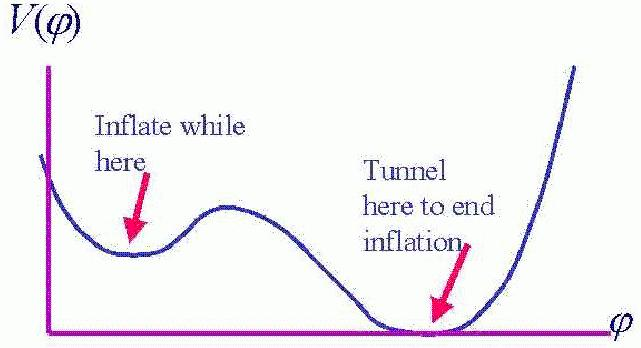
\includegraphics[width=0.5\linewidth, height=0.24\textheight]{Images/Chap2/GuthInflation_Fig5}
	\caption{Guth's potential in the old inflation. The inflation is achieved when the inflaton field is trapped in the false vacuum \cite{Chap2:Fig1}. }
	\label{fig:guthinflationfig5}
\end{figure}

Then, with a good appriximation, we can rewrite the energy density $ (\ref{Chap2EnergyDensity}) $ as 
\begin{equation}
	\label{Chap2:NewEnergyDensity}
	\rho(T)=\frac{\pi^{2}}{30}g_{*}(T)T^{4} + \rho_{0},
\end{equation}
where the value of $ \rho_{0} $ is positive and is determined by the particle theory.\\
We can rewrite (\ref{Chap2:Friedmann-Temperature}) as
\begin{equation}
\label{Chap2:Temperature-EnergydensityModified}
\Big(\frac{\dot{T}}{T}\Big)^{2}=\frac{4\pi^{2}}{45}Gg_{*}(T)T^{4}+\frac{8\pi G}{3}\rho_{0}.
\end{equation}
When the temperature is low enough the $ \rho_{0} $ term dominates over the other term in the RHS of the equation, and one has

\begin{equation}
	T(t)\simeq const \times e^{-\xi t}
\end{equation} 

where 

\begin{equation}
	\label{Chap2:psi}
	\xi^{2} =\frac{8\pi G}{3}\rho_{0}.
\end{equation}

Suppose that this supercooling continues down to some temperature $ T_{s} $, many orders of magnitude below $ T_{c} $.
Since from (\ref{Chap2:Friedmann-Temperature}) we have $ aT=const $, we finally obtain
\begin{equation}
	\label{Chap2:Expansion}
	a(t)=const \times e^{\xi t}.
\end{equation}
The universe is expanding exponentially, in a false vacuum state of energy density $\rho_{0}$.\\ In other words: if we consider initially the universe in thermal equilibrium (at least locally, in some regions), then when the temperature of such regions falls below $ T_{c} $ the effective potential of the inflaton field changes and at least another minimum  of the potential appears (true vacuum). However, the inflaton initially remains in the false vacuum and we have inflation.\\  
The universe will continue to supercool as it expands. Suppose that this cooling continues down to some temperature $ T_{s} $, many orders of magnitude below $ T_{c} $. When the field passes from the false vacuum to the true vacuum (by means quantum tunneling or in a classical way), the system undergoes a phase transition of the first order by means the generation of bubbles. When finally the phase transition takes place at $ T_{s} $ the latent heat is released and the universe is reheated at some temperature comparable to $ T_{c} $. We have the reheating stage.\\ 
As the universe expands and cools through the critical temperature $ T_{c} $ we have a nucleation of bubbles caused by the tunneling of the inflaton field from the false vacumm to the true one. The bubbles form randomly and we can introduce a certain nucleation rate $ \lambda(t) $, which is the probability per (physical) volume per time that a bubble will form in any region which is still in the high-temperature phase. We can imagine that the bubbles start at a point and expand at the speed of light. 
The crucial issue of this picture is that to solve the horizon and flatness problems the nucleation rate $ \lambda(t) $ needs to be slow compared to the expansion rate of the universe. This leads to disastrous consequences.\\
First af all, the latent heat released as a bubble expands is transferred initially to the walls of the bubble. This energy can be thermalized only when the bubbles walls undergo many collisions. As time goes on, we obtain regions of the universe occupied by separated clusters of these bubbles that grow in size. The range of these bubbles is immense. However, in these regions the clusters do not join together to form an infinite region (\textit{percolation}). It can be shown that the system percolates for large values of $ \lambda/\xi^{4} $, but for sufficiently small values it does not.\\
Without a sufficient collision of these bubbles we obtain an extremely dishomogeneous universe, far away from the current observations.

\subsection{Chaotic Inflation}
Consider a theory of a scalar field $\phi$ with effective potential $ V(\phi)=V_{0} = const > 0$. There are no reasons to expect that the classical field $\phi$ is equal to any particular value (e.g. $\phi = 0$) in the entire early universe. Instead, we expect that all values of the field $\phi$ may appears in different regions, with equal probability, varying from  $ -\infty $ to $ +\infty $ in different points of the universe. This is the idea of the \textit{Chaotic Inflation} \cite{ChaoticInflationLinde:Chap2}.\\
The only constraint we assume on the field $\phi$ in the early universe is that $ (\partial_{\mu} \phi)^{2} \le M_{P}^{2} $ for $ \mu = 0,1,2,3 $, since otherwise the corresponding part of the universe would be in the pre-planckian era, in which the classical description is impossible.\\
For example we can study the simplest model of a scalar field $\phi$ with a mass $ m $ and with the potential energy density $ V(\phi) = \frac{m^{2}}{2}\phi^{2} $ (fig. \ref{fig:chaoticinflationgwfrominflationfig3}).
\begin{figure}
	\centering
	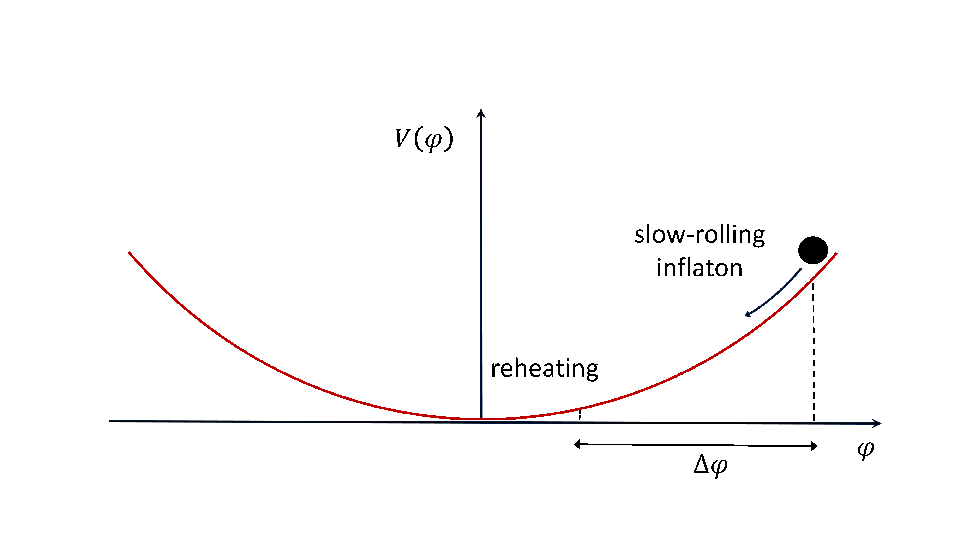
\includegraphics[width=0.55\linewidth, height=0.24\textheight]{Images/Chap2/ChaoticInflation_GWFromInflation_Fig3}
	\caption{Example of chaotic inflation potential. $ \Delta \phi $  indicates the inflaton excursion between the horizon exit of a given comoving scale and the end of inflation. Chaotic inflation is an example of \textit{large-field models} \cite{GWFromInflation:Intro}.}
	\label{fig:chaoticinflationgwfrominflationfig3}
\end{figure}
 Accountig for the expansion of the universe with Hubble constant $ H=\dot{a}/a $, the system is described by the equation of motion of the field $\phi$
\begin{equation}
	\label{Chap2eomChaoticInflation}
	\ddot{\phi} + 3H\dot{\phi} = -m^{2}\phi. 
\end{equation}
As said, the second term in the LHS of this equation can be interpreted as a friction term. The Friedmann equation (\ref{friedmannEquations1Chap2}) for a homogeneous universe containing the scalar field $\phi$ yields

\begin{equation}
	\label{Chap2:friedmannChaoticInflation}
	H^{2}=\frac{8 \pi G}{3}\rho_{\phi}= \frac{4 \pi G}{3}\Big (\dot{\phi}^{2} + m^{2}\phi^{2} \Big )
\end{equation}
where we have used (\ref{energyDensityPressure}) and neglected the curvature term.\\
From the last equation we see that if the scalar field $\phi$ initially was large, the Hubble parameter $ H $ had to be large too and then the friction term. This means that the scalar field during inflation was moving very slowly, as a ball in a viscous liquid. Therefore the energy density of the inflaton, unlike the density of ordinary matter, remained almost constant, and the expansion of the universe continued with a high speed. \\
Soon after the beginning of this regime (rapid expansion of the universe and slow motion of $\phi$) we obtain $ \ddot{\phi} \ll 3H\dot{\phi} $, $\dot{\phi^{2}}$ $\ll$ $ m^{2}\phi^{2} $, yielding
\begin{equation}
	\label{Chap2:HubbleRateField}
	H=\frac{\dot{a}}{a} =\sqrt{\frac{4\pi G}{3}}m\phi.
\end{equation}
 This equation shows that if the field $\phi$ changes slowly the size of the universe in this regime grows approximately as $ e^{H t} $ with $ H $ given by (\ref{Chap2:HubbleRateField}). \\
 In this model inflation does not require initial state of thermal equilibrium, supercooling and tunnelling from the false vacuum. This means that, in this scenario, there is no bubble nucleation and then the problems seen with Guth's model are avoided.\\
 When inflation ends, the scalar field $\phi$ begins to oscillate near the minimun of $ V(\phi) $. As any rapidly oscillating classical field, it looses its energy by creating pairs of elementary particles. These particles interact with each other and come to a state of thermal equilibrium with some temperature $ T_{r} $. From this time on, the universe can be described by the usual big bang theory.\\
 To have an idea of the huge expansion of the universe during inflation we can consider the mass $ m $ of the inflaton about $ 10^{-6} M_{p} $ and an initially closed universe with initial size $ l \simeq M_{p}^{-1} $. Moreover, we assume as initial condition for the energy density $\rho \simeq 1$ of the scalar field. From $\rho < 1$ we can consider this domain as classical universe.\\
 Solving (\ref{Chap2:HubbleRateField}) comes out that the total amount of inflation achieved starting from $ V(\phi) \simeq 1 $ is of the order of $ 10^{10^{10}} $ ! . In this model the total duration of inflation is about $ 10^{-30} $ seconds. From investigations of this period, if we consider the initial size of the universe small as the Planck size $ l_{p} $ $\simeq 10^{-33} cm$, after $ 10^{-30} $ seconds of inflation the universe acquires a huge size of $ l \simeq 10^{10^{10}} cm $ \cite{Chap2:Linde_HystoryInflation}. This value is model dependent, but in all realistic models  the size of the universe after inflation appears to be many orders of magnitude greater than the size of the part of the universe which we can see now, $ l \simeq 10^{28} cm $. Thus, most of the problems of the old cosmological theories are immediatly solved. \\
 If the universe initially consisted of many domains with chaotically distributed scalar field $\phi$, then domains with a value of the inflaton too small never inflated. Thus, the main contribution is given by those domains which originally contained large scalar field $\phi$. Inflation of such domains creates very large homogeneous islands out of initial chaos, each one much greater than the size of the observable part of the universe.\\
 Other examples of models of chaotic inflation are based on polynomial potentials. The first potential proposed by Linde, when he suggested the chaotic inflation scenario, was $ V(\phi) = \frac{\lambda}{4} \phi^{4} $ \cite{ChaoticInflationLinde:Chap2}. However, the main idea of this type of inflation is quite generic. One can consider any particular potential $ V(\phi) $, polynomial or not, with or without spontaneous symmetry breaking, and study all possible initial conditions without assuming that the universe was in a state of thermal equilibrium. 
 
 \subsection{Small-field models}
 The small field models are characterized by the following potential around $\phi=0$:
 \begin{equation}
 	\label{Chap2:small-field1}
 	V(\phi) = V_{0}\Big [1-\Big (\frac{\phi}{\mu}\Big)^{n} \Big]
 \end{equation}
which may arise in spontaneous symmetry breaking.
An important example is \textit{Natural Inflation} model where a Pseudo Nambu-Goldstone boson (PNGB) playes the role of inflaton \cite{Chap2:NaturalInflation}. The PNGB potential is in  the form
\begin{equation}
	\label{Chap2:PNGBPotential}
	V(\phi) = \Lambda^{4}\big [1 + cos(\phi/f) \big],
\end{equation}  
 where the two mass scales $\Lambda$ and $ f $ characterize the height and width of the potential, respectevely (fig. \ref{fig:naturalinflationinflationdynamics-and-reheating}). The potential has a unique minimun at $ \phi = \pi f $. The typical mass scales for successful inflation are of order  $ f \sim M_{pl} \sim 10^{19} $ Gev and $ \Lambda \sim m_{GUT} \sim 10^{16} Gev $. For temperatures $ T \le f $ the global symmetry is spontaneously broken. These mass scales arise in particle physics models, for example in superstring theories. \\
 \begin{figure}
 	\centering
 	\includegraphics[width=0.5\linewidth, height=0.25\textheight]{"Images/Chap2/NaturalInflation_InflationDynamics and reheating"}
 	\caption{Natural inflation potential. This is an example of \textit{small-field model} \cite{InflationDynamicsAndReheating:chap1}.}
 	\label{fig:naturalinflationinflationdynamics-and-reheating}
 \end{figure}
  We can describe the evolution of the field as 
 \begin{equation}
 	\label{Chap2:eomSmallFieldModel}
 	\ddot{\phi} + 3H\dot{\phi} + \Gamma\dot{\phi} + V'(\phi) = 0,
 \end{equation} 
where $\Gamma$ is the decay rate of the inflaton.\\
When the temperature T $\le$ $\Lambda$, in regions of the universe with $\phi$ initially near the top of the potential, the field starts to slowly roll down toward the minimun of the potential. In those regions, the energy density of the universe is quickly dominated by the vacuum contribution and the universe expands exponentially. The slow-roll regime is characterized,  as in the previous models, by $ \ddot{\phi} \ll 3H\dot{\phi} $ and the initial condition for the field $\phi$, as in chaotic scenario, are random. \\
At the end of the slow-roll regime we have the reheating phase. The field $\phi$ begins to oscillate about the minimun of the potential, and gives rise to particle and entropy production. .
During this process the energy of the inflaton is converted in radiation in a time $\simeq \Gamma^{-1}$. If $\Gamma > H$, then the reheating process takes less than an expansion time ($\simeq H^{-1}$), and the coherent field energy is efficiently converted to radiation, reheating the universe to a temperature \cite{Chap2:NaturalInflation_Turner_Steinhardt}
\begin{equation}
\label{Chap2:ReheatingTemperatureSmallFieldModel}
T_{RH}=\Big (\frac{45}{4\pi^{3}g_{*}}\Big )^{1/4} (Hm_{pl})^{1/2}
\end{equation}
where $ g_{*} $ counts the effective number of relativistic degree of freedom.\\
On the other hand, if $ \Gamma < H $, then the reheating process takes longer than an expansion time. Until $ t \simeq \Gamma^{-1} $ the field continues to oscillate about the minimun of the potential. When $ t \simeq \Gamma^{-1} $ these oscillations are damped (in a few expansion times), reheating the universe to a temperature
\begin{equation}
	T_{RH} \simeq \Big (\frac{45}{4\pi^{3}g_{*}}\Big)^{1/4}(\Gamma m_{pl})^{1/2}.
\end{equation}

The decay rate can be evaluated as 
\begin{equation}
	\label{Chap2:DecayRate}
	\Gamma \simeq g^{2}\Lambda^{6}/f^{5}
\end{equation}
where g is an effective coupling constant (for example, in the axion model \cite{Chap2:AxionModel}, $ g \propto \alpha_{EM} $ for two-photon decay). For $ f=m_{pl} $ and $ g_{*}=10^{3} $, we find that $ T_{RH} \simeq 10^{14}\ Gev $ in the first case ($ \Gamma > H $) and $ T_{RH} \simeq 10^{8} g\ Gev$ in the other case ($\Gamma < H$). Since generally we expect that $ g < 1 $, the reheating temperature will be $ T_{RH} < 10^{8}\ Gev $ \cite{Chap2:NaturalInflation}.\\
This can have very insteresting application in GUT baryogenesis models (see \cite{Chap2:NaturalInflation} and \cite{Chap2:NaturalInflation_Turner_Steinhardt}).

\subsection{Hybrid models}
In this type of model the inflation ends because of the combination of several scalar fields. In particular, we have a scenario with two interacting scalar fields where inflation ends by a rapid rolling (\textit{waterfall}) of a second scalar field $\sigma$ besides the inflaton, triggered by the slow rolling of the field $\phi$ \cite{Chap2: Hybrid_Model}.\\
An example of effective potential from this type of model is given by
\begin{equation}
\label{Chap2:Hybrid model}
	V(\sigma,\phi) = \frac{1}{4\lambda}(M^{2}-\lambda \sigma^{2})^{2} + \frac{m^{2}}{2}\phi^{2} + \frac{g^{2}}{2}\phi^{2}\sigma^{2} 
\end{equation} 
When the fields have large value their effective mass squared are both positive and the potential has the symmetry $ \sigma \leftrightarrow -\sigma $. The potential has a maximum at $\phi = \sigma = 0$ and a global minimum at $\phi = 0$, $\sigma=\sigma_{0}=M/\sqrt{\lambda }$ where the symmetry is broken.\\
The effective mass squared of the field $\sigma$ is obtained by deriving the potential two times with respect the field $\sigma$:
\begin{equation}
	\label{massEffectiveSigma}
	m^{2}_{\sigma} = V''_{\sigma}(\sigma,\phi) = -M^{2} + g^{2}\phi^{2}.
\end{equation}
 Since the curvature of the effective potential in the $\sigma$-direction is much greater than in the $\phi$-direction we expect that at the first stages of expansion of the universe the field $\sigma$ rolled down to $\sigma=0$, whereas the field $\phi$ could remain large for longer time. Thus, we can consider the motion starting at large $\phi$ (where the effective mass of the $\sigma$ field is large) and the field is sitting at the minimum of the potential at $\sigma=0$.\\
 During the slow-roll of the field $\phi$, the effective mass of the triggering field is $ m^{2}_{\sigma} = g^{2}\phi^{2}-M^{2}$. As soon as the field $\phi$ acquires the critical value $\phi_{c}=M/g$, fluctuations of the massless $\sigma$ field trigger the symmetry breaking phase and inflation ends. \\
 \begin{figure}
 	\centering
 	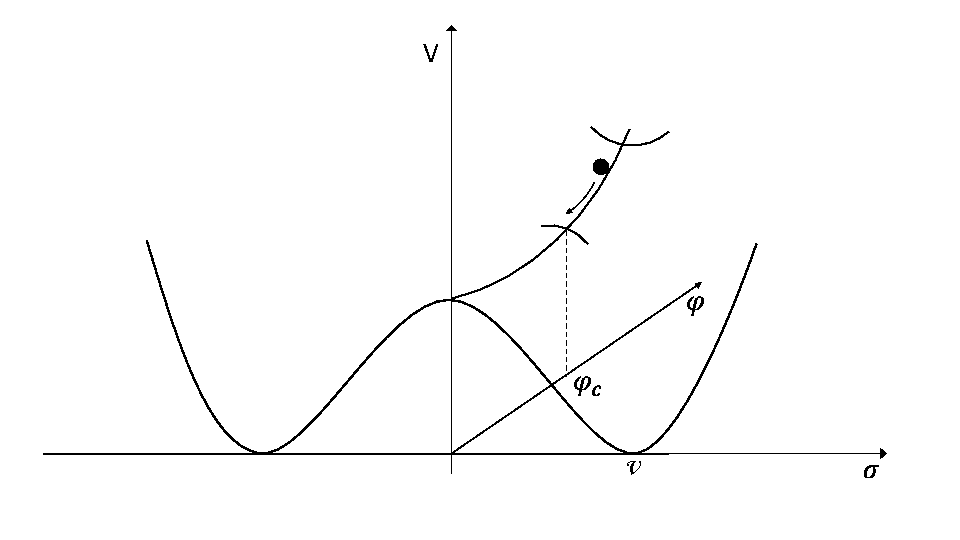
\includegraphics[width=0.55\linewidth, height=0.25\textheight]{Images/Chap2/HybridModel_GWFromInflation_Fig4}
 	\caption{Hybrid inflation potential. The field rolls down the potential up to the critical value $\phi_{c}$, and then reaches the true minimum of the potential $ \phi=0,\sigma=\sigma_{0}=v$ \cite{GWFromInflation:Intro}}
 	\label{fig:hybridmodelgwfrominflationfig4}.
 \end{figure} 
 If the bare mass $ M $ is large compared with the rate of expansion $H$ of the universe, the transition will be instantaneous and inflation will end very rapidly. Instead, if the $ M $ parameter is of the order of $ H $, then the transition will be very slow and we can have a few more e-folds of inflation after the phase transition. When $ \sigma=0 $ the effective potential becomes
 \begin{equation}
 \label{effectivePotential}
 V(\phi)=\frac{M^{4}}{4\lambda} +  \frac{m^{2} \phi^{2}}{2}.
 \end{equation}
Since during inflation the scalar field $\phi$ is of the order $\phi_{c}=M/g$, if $ m^{2} \ll g^{2}M^{2}/\lambda $ we obtain for the potential the expression
\begin{equation}
	\label{potential}
	V(\phi,0)=\frac{M^{4}}{4\lambda} +  \frac{m^{2} \phi^{2}}{2} \simeq \frac{M^{4}}{4\lambda},
\end{equation} 
and for the Hubble rate, under this condition,
\begin{equation}
	\label{Chap2:HubbleHybrid}
	H^{2}\simeq\frac{8\pi G}{3} V(\phi,0) \simeq \frac{8\pi }{3M_{pl}^{2}}\frac{M^{4}}{4\lambda} =\frac{2\pi M^{4}}{3\lambda M_{pl}^{2}.}
\end{equation}
This means that, under the condition $  m^{2} \ll g^{2}M^{2}/\lambda $, we obtain inflation for $ \phi > \phi_{c} $. In this case the inflation is driven by the vacuum energy density $ V(0,0) = M^{4}/4\lambda $.\\
The complete equation of motion of the field $\phi$ is
\begin{equation}
	\ddot{\phi} + 3H\dot{\phi}=-(m^{2} + g^{2}\sigma^{2})\phi.
\end{equation}
As said, during inflation $\sigma=0$ and one can neglect $\ddot{\phi}$ in the equation of motion for the field $\phi$, yielding
\begin{equation}
	\label{eom}
	3H\dot{\phi}=-m^{2}\phi.
\end{equation}
It is then possible to integrate the evolution equation of $\phi$, obtaining
\begin{equation}	
	\label{Chap2:solutionField}
	\phi(N)=\phi_{c}e^{rN}, \qquad r\simeq \frac{m^{2}}{3H^{2}}
\end{equation}
where $ N=H(t_{c}-t) $ is the number of e-folds to the phase transition.\\
We can study the beheaviour of the field $\phi$ and $\sigma$ after the time 
$ \Delta t = H^{-1}=\sqrt{\frac{3\lambda}{2\pi}}\frac{M_{pl}}{M^{2}} $ from the moment $ t_{c} $ when the field $\phi$ becomes equal to $\phi_{c}$.
Considering the equation of motion of the field during inflation (\ref{eom}), during the time $\Delta t$ the variation $\Delta \phi$ is
\begin{equation}
	\label{Chap2:variationDeltaPhi}
	\Delta \phi = \frac{m^{2} \phi_{c}}{3H^{2}} = \frac{m^{2}M}{3H^{2}g} = \frac{\lambda m^{2}M_{pl}^{2}}{2\pi gM^{3}}.
\end{equation}

Thus, the value of the field after $\Delta t$ becomes
\begin{equation}
	\label{Chap2:fieldSquare}
	\phi_{t_{c}-\Delta\phi}=\frac{M}{g}\Big (1-\frac{\lambda m^{2} M^{2}_{pl}} {2\pi M^{4}} \Big ).
\end{equation}
Moreover, after $ t_{c} - \Delta t $ the value of the negative mass squared of the field $\sigma$ (\ref{massEffectiveSigma}) becomes
\begin{equation}
	\label{Chap2}
	m^{2}_{\sigma} = - M^{2}(\phi) = - \frac{\lambda m^{2}M^{2}_{pl}}{\pi M^{2}} 
\end{equation}
where the square of the field $\phi$ is obtained expanding the square of (\ref{Chap2:fieldSquare}) (we are working in the regime $ M^{2} \gg \lambda m^{2}/g^{2} $).\\
The value of $ M^{2}(\phi) $ is much greater than $ H^{2} $ for $ M^{3} \ll \lambda m M_{pl}^{2} $ (see (\ref{Chap2:HubbleHybrid})). This means that the field $\sigma$ within the time $\Delta t \sim H^{-1} $ rolls down to its minimum at $\sigma (\phi) = M(\phi)/\sqrt{\lambda}$, rapidly oscillates near it and loses its energy  due to the expansion of the universe.\\
It can be checked that the field $\phi$ rolls down very fast towards the minimum of its effective potential within a time much smaller than $ H^{-1} $ if $ M^{3} \ll \sqrt{\lambda}gmM_{pl}^{2} $.\\
Thus, under these conditions inflation ends in this theory almost instantaneously, as soon as the field $\phi$ reaches the critical value $\phi_{c} = M/g$.\\
Considering the reheating phase at the end of this type of model it will be important the following consideration. According to the classical equation of motion, the field $ \sigma=0 $ cannot change its value because the first derivative of the effective potential at $\sigma=0$ vanishes. The spontaneous symmetry braking  in this case occurs due to the exponential growth of quantum fluctuations. Indeed, writing the (negative) effective mass squared of the field $ -m^{2}_{\sigma}(\phi)=g^{2}(\phi-\phi_{c}) $ we immediately see that it vanishes at the critical point, but becomes large and grows up to $ m^{2}_{\sigma}(0) = M $ as the field $\phi$ slides towards $\phi=0$. This leads to a fast growing of quantum fluctuations of the scalar field $\sigma$, producing an inhomogeneous distribution of the field $\sigma$ with $ <\sigma>=0 $. We'll return to this in a more detailed way later. \\
Quantum fluctuations of the inflaton field produce metric perturbations $ \mathcal{R} \simeq H\delta\phi/\dot{\phi} $, where $\delta \phi$ is the amplitude of the field fluctuations when they cross outside the Hubble scale.
Appying (\ref{PR}) with the solution (\ref{Chap2:solutionField}) we obtain
\begin{equation}
\dot{\phi}=-(Hr\phi_{c})e^{rN},	
\end{equation}
and 
\begin{equation}
	\label{Chap2:P_{R}}
	P_{\mathcal{R}}=\Big (\frac{H^{2}}{4\pi^{2}r^{2}\phi_{c}^{2}}\Big)e^{-2rN} = \frac{1}{r^{2}}\frac{g^{2}M^{2}}{6\pi\lambda M_{pl}^{2}}e^{-2rN}.
\end{equation}

However, another more accurate way to compute this spectrum (\ref{Chap2:P_{R}}) is in \cite{Chap2:PerturbationsHybridInflation}. The only difference is that the spectrum (\ref{Chap2:P_{R}}) is multiplied by $ C(r)^{2} $ where $ C(r)=\Gamma[3/2-r]/2^{r}\Gamma[3/2] $ $\simeq 1$ in the limit $ m\ll H $.
Moreover, \cite{Chap2:PerturbationsHybridInflation} evaluated the spectral tilt as
\begin{equation}
	n_{\mathcal{R}} - 1 = \frac{d\ ln\ P_{\mathcal{R}}}{d\ ln\ k} = 2r. 
\end{equation}
Note that the tilt is always greater than one in this model.\\
The hybrid inflation is also a version of the chaotic inflation scenario. The main difference between this scenario and the simplest versions of the one-field chaotic inflation is in the way inflation ends. In the theory with  a single field, inflation ends when the potential of this field becomes steep. In the hybrid picture, instead, inflation ends due to the presence of another scalar field that triggers the waterfall.\\
Several extensions of this scenario became quite popular in the context of supergravity and string cosmology.

\section{Observations}
Inflation is not just an interesting theory  that can resolve many problems of the standard Big-Bang cosmology. The inflation paradigm made several predictions which can be tested by cosmological observations.\\
The first important prediction is that the universe must be flat and in most models $ \Omega = 1 \pm 10^{-4} $.\\
 An other important prediction is that  inflationary perturbations generated during a slow-roll regime with $\epsilon,\eta$ $\ll 1$ have a nearly flat spectrum with $ n_{S}$ close to 1. In general the spectrum of inflationary perturbations usually is slightly non-flat. It is possibile to construct models with $ n_{S}$ extremely close (or even exactly equal) to 1, but the small deviation of the spectrum from the exact flatness is one of the distinguishing features of inflation.\\
 Perturbations of the metric could be scalar, vector or tensor. Inflation mostly produces scalar perturbations, but it also produces tensor perturbations with nearly flat spectrum, and it does not produce vector perturbations. As seen in the first chapter  there are important relations between the scalar and tensor perturbations produced by inflation.\\
 The perturbations coming from inflation produce specific peaks in the spectrum of CMB radiation.\\
 It is possible to violate each of these predictions if one makes inflationary theory sufficiently complicated. For example, it is possible to produce vector perturbations of the metric in the models where cosmic strings are produced at the end of inflation, which is the case of some other models of hybrid inflation. However, it is difficult to do so, and most of the inflationary models obey the predictions above \cite{Chap2:Linde_HystoryInflation}.\\
 The most recent constraints on inflation comes from the 2018 $ Planck $ measurements of the CMB anisotropies \cite{Chap2:Planck2018}. The \textit{Planck} mission estimates the spectral index as
 \begin{equation}
 	\label{spectral index}
 	n_{s}= 0.9626 \pm 0.0057  \qquad (68\% C.L.).
 \end{equation}
and the curvature constraint
 \begin{equation}
 	\label{curvatureConstraint}
 	\Omega_{K}= 0.0007 \pm 0.0037 \qquad  (95\% C.L). 
 \end{equation}
Moreover, the tensor-to-scalar ratio $ r $ is estimated, assuming that it satisfies the consistency relation  ($ n_{T} = -r/8 $),
\begin{equation}
	r_{0.02} < 0.056 \qquad (95\% C.L.).
\end{equation}
To characterize the system we can write the power spectra w.r.t a pivot scale $ k_{0} $ as power laws
\begin{equation}
	\Delta_{T}(k) = \Delta_{T}(k_{0})\Big (\frac{k}{k_{0}}\Big)^{n_{T}} \qquad \Delta(k) = \Delta_{\zeta}(k_{0})\Big (\frac{k}{k_{0}}\Big)^{n_{s}-1}
\end{equation}
obtaining a set of 4 observables: 2 spectral indeces and 2 amplitudes.\\
Assuming the consistency relation true we can reduce the DOF to 3.  Exploiting the normalitation of CMB anisotropies on large angular scales $ \Delta T/T \sim 10^{-5}$ \cite{Chap2:Wilkinson}, one can constraint one of the two amplitudes since it contains both $\zeta$ and GW contributions.
From experimental constraints on amplitudes and spectral indeces we can also constraint  the slow-roll parameters since $ n_{T}=-2\epsilon $ and $ n_{S}-1=2\eta - 6\epsilon $.\\
The usually chosen DOF to classify inflationary models are taken to be $ (r,n_{s}) $, from which we build the parameter space.\\
In the $ (r,n_{s}) $ plane, we have that different classes of models (small-field, large-field, hybrid models) occupy different regions. Indeed, we can consider  the parameter $\eta\simeq M_{pl}V''/V$ and rewriting the tensor-to-scalar ratio in terms of the slow-roll parameters as $r=16\epsilon$ we obtain


\begin{equation}
	r(n_{s},\eta)=\frac{8}{3}(1-n_{s}) + \frac{2}{3\pi}M_{pl}^{2}\frac{V''}{V}.
\end{equation}
For $\eta < 0 $ we have small-field models, for $ 0<\eta<2\epsilon $ we have  large-field models and hybrid models provide $\eta>2\epsilon $. The hybrid models are almost excluded by observation yielding $ n_{s} \le 1 $.
As mentioned, even if we are considering only the simplest models which realise inflation, there is still a large variety of them ("zoology"). In addition, one can see that the large field models tend to produce more gravitational waves than small ones.
\begin{figure}
	\centering
	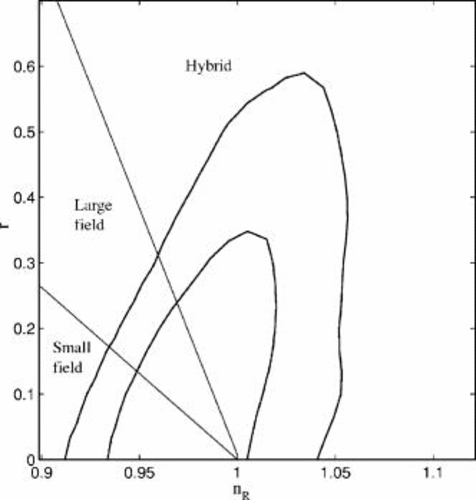
\includegraphics[width=0.6\linewidth, height=0.3\textheight]{Images/Chap2/r_ns_InflDynamicsAndReheating}
	\caption{Classification of inflationary models in the $ n_{\mathcal{R}}-r $ plane. The line $ r = (8/3)(1-n_{\mathcal{R}}) $ marks the border of large-field and small-field models,  whereas  the border of large-field and hybrid models correspond to $ r=8(1-n_\mathcal{R}) $ \cite{InflationDynamicsAndReheating:chap1}.}
	\label{fig:rnsinfldynamicsandreheating}
\end{figure}



\section{Reheating}
In this section we start to discuss one of the main focus of this thesis: The reheating stage after inflation.\\
As said, after  inflation the standard FLRW  radiation dominated universe should start, in order to recover the standard Big-Bang model of the universe. However, during the accelerated expansion of the universe $ T \propto a^{-1} \simeq e^{-Ht} $. Then, at the end of inflation the temperature becomes too small to allow a good thermalitation of the particles and then start the radiation dominated era. This is the reason why we need a post-inflation period in which the universe is reheated and which comes just before the radiation dominated era.\\
For now, we present a toy, elementary model of reheating. From Chapter 4 we'll investigate deeply such period and we will see, actually, that this phase leads to very interesting non-linear physics and dynamics. For reference see \cite{Chap2:Kolb_Turner}.\\
We start considering the simple single-field model discussed in the first chapter
\begin{equation}
		\mathcal{L} = -\dfrac{1}{2} g^{\mu\nu} \partial_{\mu}\phi \partial_{\nu} \phi - V(\phi).
\end{equation}	
Inflation ends when the slow-roll parameter $\epsilon$ reaches the value 1, which implies that also $\eta=1$. Indeed, this happens when the curvature $ V'' $ of the potential stars to become non negligible, implying that the flat region in which the slow-roll takes place has ended. This stage is equivalent to say that $ V''\sim H^{2} $, that means $\eta \sim 1$ from (\ref{eta2}) (we recall that we have renaimed $\eta_{V}$ as $\eta$). \\
From this moment the second derivative of the potential starts to increase, becoming greater than the rate of the expansion of the universe, and the inflaton begins to oscillate around the minimun with an high frequency $\omega$. This leads to $ V'' \propto \omega^{2} \gg H^{2} $.
Moreover, the inflaton not only starts to oscillate with high frequency around the minimum of the potential but it also decays with a rate $\Gamma_{\phi}$ to lighter relativistic particles that reheat the universe.\\
We can then modify the equation of motion for the inflaton field in a way that takes into account its decay
\begin{equation}
	\label{Chap2:EOM_Modified}
	\ddot{\phi} + (3H + \Gamma_{\phi})\dot{\phi} + V'(\phi) = 0.
\end{equation}
We remark that the decay rate is a rate such as $H  $  and then they should be multiplied by $\dot{\phi}$.\\
Consider now the energy density of the inflaton $\rho_{\phi} = \frac{1}{2} \dot{\phi^{2}} + V(\phi)$ and compute the time derivative
\begin{equation}
	\label{Chap2:dotPhi}
	\dot{\rho_{\phi}}=\dot{\phi}\ddot{\phi} + V'\dot{\phi}.
\end{equation}
Multiplying (\ref{Chap2:EOM_Modified}) by $\dot{\phi}$ and using the last expression, we obtain
\begin{equation}
	\label{Chap2:dotPhiEquation}
	\dot{\rho_{\phi}} + \dot{\phi^{2}}(3H^{2} + \Gamma_{\phi}) = 0
\end{equation}
Moreover, using the fact that the typical time of oscillation is much smaller than the characteristic time of expansion, we can take an average over a period of oscillation such as
\begin{equation}
	\label{Chap2:oscillationAverage}
	\dfrac{1}{2} <\dot{\phi^{2}}>_{period}\ =\ <V(\phi)>_{period}\qquad \rightarrow\qquad \rho_{\phi}\ =\ <\dot{\phi^{2}}>_{period}
\end{equation}
Finally, the final form of (\ref{Chap2:dotPhiEquation}) reads
\begin{equation}
	\label{Chap2:FinalEqRho}
\dot{\rho}_{\phi} + (3H + \Gamma_{\phi})\rho_{\phi} = 0	.
\end{equation}
To solve this equation we consider the general solution
\begin{equation}
	\label{Chap2:rhoSolution1}
	\rho_{\phi}(t)=\rho_{osc}e^{-A(t)}, \qquad A(t)=\int_{t_{osc}}^{t}(3H+\Gamma_{\phi})dt
\end{equation}
where $ \rho_{osc} $ denotes the initial condition at $ t_{osc} $, the time at which the inflaton begins to oscillate. The solution for $ A(t) $ reads
\begin{equation}
	\label{Chap2:solutionAt)}
	A(t)= \int_{t_{osc}}^{t}\Big (3 \frac{\dot{a}}{a} + \Gamma_{\phi}\Big) dt = 3 \ln \Big(\frac{a(t)}{a_{osc}}\Big) + \Gamma_{\phi}(t-t_{osc})
\end{equation}
and, substituing in (\ref{Chap2:rhoSolution1}), we finally obtain the solution
\begin{equation}
\label{Chap2:rhoSolution}
\rho_{\phi} = \rho_{osc} \Big (\frac{a}{a_{osc}}\Big)^{-3}e^{-(t-t_{osc})\Gamma_{\phi}}.	
\end{equation}
From this equation we obtain an interesting feature of this system: during the oscillation phase the inflaton beheaves as non-relativistic pressureless matter. Moreover, we can impose as initial condition $ \rho_{osc}=M^{4} $.
The exponential extra factor accounts for the decay of the field.\\
We can summarize the situation. After the end of inflation, as a consequence of the no-more negligible curvature of the potential, the inflaton field moves towards the minimum and starts to oscillate around it with an high frequency. At times $ t $ near to $ t_{osc} $ the decay of $\phi$ is not efficient and $\rho_{\phi}$ decreases essentially as $ a^{-3} $. However, the field $\phi$ starts to decay, with a rate $\Gamma_{\phi}$. Because of these contributions the energy density of the inflaton decreases, but still dominates the energy density of the universe. As time passes, the decay starts to become important and  at $ t_{decay} \sim 1/\Gamma_{\phi} $ becomes very efficient.
At this point the energy density of the inflaton starts to be very strongly suppressed and that of the relativistic particles increases.\\
The presence of the new term $\Gamma_{\phi}$ related  to the decay of the inflaton field brings to a modification also to the equation for the energy density of radiation, which becomes
\begin{equation}
	\label{Chap2:radiationEquation}
	\dot{\rho_{r}} + 4H\rho_{r} = \Gamma_{\phi}\rho_{\phi}.
\end{equation}
As we said, from $ t_{osc} \simeq H^{-1} \simeq M_{pl}/M^{2} $ to $ t_{decay} \simeq \Gamma^{-1} $ the field oscillates but, although in principle it can decay, this process is still not efficient. Lighter particles begin to be produced in a slow way and their energy is still dominated by that of the inflaton, which energy continues to decrease.\\
As a consequence of this peculiar phase $\rho_{r}$ has not the particular beheaviour $ a^{-4} $ which is expected from the standard radiation dominated era, but the universe is still dominated by a matter-like field. In such phase the scale factor evolves as $ a \propto t^{2/3} $ and the Hubble constant reads $ H=2/3t $.\\
Thus, starting from (\ref{Chap2:radiationEquation}) we can write
\begin{equation}
	\label{Chap2:radiationEquation2}
	\dot{\rho_{r}} + \frac{8}{3t}\rho_{r}\simeq \Gamma_{\phi}\rho_{osc}\Big (\frac{a}{a_{osc}}\Big)^{-3}
\end{equation}
where we have evaluated the expression near $ t_{osc} \sim M_{pl}/M^{2} $, neglecting the exponential term in $\rho_{\phi}$. Considering the time beheaviour of the scale factor  and $\rho_{osc}=M^{4}$ this equation yields
\begin{equation}
	\label{Chap2:radiation3}
		\dot{\rho_{r}} + \frac{8}{3t}\rho_{r} \simeq \Gamma_{\phi} M^{4} \Big (\frac{t}{t_{osc}}\Big)^{-2} \simeq \frac{\Gamma_{\phi} M_{pl}^{2}}{t^{2}}
\end{equation}
To solve this equation we can search solution for $ \rho_{r} \propto t^{\alpha} $, taking as initial condition $\rho_{r}(t_{osc})=0$. We can use also the general solution
\begin{equation}
	\label{Chap2:generalSolution}
	\rho_{r}(t)=c_{in}e^{-A(t)} + e^{-A(t)} \int_{t_{osc}}^{t}dt'\ (g(t')e^{A(t')}), \qquad 
	g(t') = \frac{\Gamma_{\phi} M_{pl}^{2}}{t'^{2}}  
\end{equation}
where $ c_{in} $ denotes the initial condition. Putting $ \rho(t_{osc})=0 $ it is easy to see that $ c_{in}=0 $. The $ A(t) $ term is given by
\begin{equation}
	\label{Chap2:A(t)2}
	A(t)=\int_{t_{osc}}^{t}\frac{8}{3t'}dt'=\frac{8}{3}\ln(t/t_{osc})
\end{equation}
Finally, the integral term in (\ref{Chap2:generalSolution}) yields
\begin{equation}
	\label{Chap2:IntegralTerm}
	\int_{t_{osc}}^{t} dt'\frac{\Gamma_{\phi} M_{pl}^{2}}{t'^{2}}\Big (\frac{t'}{t_{osc}}\Big)^{8/3} = \frac{9}{40}\frac{\Gamma_{\phi} M_{pl}^{2}}{t_{osc}^{8/3}}(t^{5/3} - t_{osc}^{5/3})
\end{equation}
Putting all inside (\ref{Chap2:generalSolution}) we obtain
\begin{equation}
	\rho_{r}=\frac{9}{40}\frac{\Gamma_{\phi}M_{pl}^{2}}{t}\Big (1- \Big (\frac{t}{t_{osc}}\Big)^{-5/3}\Big)
\end{equation}
Using the scaling beheaviour $ a \propto t^{2/3} $ we can write the last expression in terms of the scale factor, obtaining the final solution
\begin{equation}
\label{Chap2:finalSolution}
\rho_{r}(t)=\frac{9}{40}\frac{\Gamma_{\phi}M_{pl}^{2}}{t_{osc}}\Big (\frac{a}{a_{osc}}\Big)^{-3/2}\Big (1- \Big (\frac{a}{a_{osc}}\Big)^{-5/2}\Big)
\end{equation}
and, using $ t_{osc}=M_{pl}/M^{2} $
\begin{equation}
	\rho_{r}(t)=\frac{9}{40}\Gamma_{\phi}M_{pl}M^{2}\Big (\frac{a}{a_{osc}}\Big)^{-3/2}\Big (1- \Big (\frac{a}{a_{osc}}\Big)^{-5/2}\Big)
\end{equation}
From this equation we can determine easily the beheaviour of the radiation energy density. During the period of oscillation of the inflaton field the radiation energy starts to grow from zero up to a maximum value $\rho_{max} \simeq \Gamma_{\phi} M_{pl} M^{2}$ thanks to the inflaton decays. Once the maximum is reached, $\rho_{r}$ decreased as $ a^{-3/2} $, instead of the usual $ a^{-4} $.\\
Regarding the temperature we can estimate the maximum temperature reached by the radiation fluid at $\rho_{max}$ using $ \rho_{r}=(\pi^{2}/30)g_{*}T^{4} $. We obtain 
\begin{equation}
	T_{max} \sim g_{*}^{-1/4}(\rho_{r}^{max})^{1/4} \sim g_{*}^{-1/4}\Gamma_{\phi}^{1/4}M_{pl}^{1/4}M^{1/2}.
\end{equation}
During this phase the system  is still between the start of oscillations and the time at which decays become efficient. In such period we have that also the entropy increases. Indeed, the total entropy $ S = sa^{3} $ is constant only if the entropy density scales as $ s \propto a^{3} $. This happens only in a pure FLRW radiation dominated universe and we are not yet in that phase.\\
In this period 
\begin{equation}
\label{Chap2:entropy}
s \propto T^{3} \sim \rho_{r}^{3/4} \sim a^{-9/8}
\end{equation}
that leads
\begin{equation}
	\label{Chap2:totalEntropy}
	S \propto a^{15/8}.
\end{equation}
Thus, during this stage the inflaton decays producing new relativistic particles and this process causes the increasing of the entropy.\\
In the final stage we reach the time $ t_{decay} \sim \Gamma^{-1}_{\phi} $. From this moment the decay of the inflaton is efficient due to the exponential term in (\ref{Chap2:rhoSolution}). The energy density of the field $\rho_{\phi}$ decreases rapidly and $\rho_{r}$ becomes the dominant energy density allowing to recover the usual radiation dominated era in which $ \rho_{r} \propto a^{-4} $ and $ S=const $. The temperature at which the radiation energy becomes the dominant energy of the universe (and then the radiation dominated era begins) is called \textit{Reheating Temperature} $ T_{R} $. To estimate this temperature we can consider the Hubble constant during the standard radiation dominated era, and evaluating it at $ t_{decay}=\Gamma_{\phi}^{-1} $:
\begin{equation}
	\label{HubbleConstant}
	H^{2} = \Big (\frac{1}{2t}\Big)^{2} = \frac{\Gamma_{\phi}^{2}}{4} 
\end{equation}
and,
\begin{equation}
	H^{2}=\frac{8\pi }{3M_{pl}^{2}}\rho_{r}\simeq \frac{8 \pi g_{*}}{3M_{pl}^{2}}\frac{\pi^{2}}{30}T^{4}_{\ |t\simeq \Gamma_{\phi}^{-1}}.
\end{equation}
Combining the last two equations we finally derive an estimate of the reheating temperature
\begin{equation}
	\label{Chap2:reheatingTemperature}
	T_{R} \simeq 0.55g_{*}^{1/4}(\Gamma_{\phi}M_{pl})^{1/2}.
\end{equation}
where we assumed for semplicity that the radiation dominated era starts at the instant $ t_{decay} $, when the decay of the inflaton field becomes efficient.\\ 
As final comment we notice that there is no remnant of the vacuum energy density of the inflaton field, which drives the accelerated expansion of the universe. Indeed, just after inflation $\phi$ beheaves as a non-relativistic pressureless field which causes its redshifting as $ a^{3} $.\\
There is also a special case in which the reheating is istantaneous at $ \rho_{osc} \simeq M^{4} \simeq T^{4}_{R} $. This happens when at $ t_{osc} $ the decay of the inflaton field is already extremely efficient. $\phi$ will not even make a single oscillation around the minimun transformig immediately all the vacuum energy directly into radiation. In this special case we have $ T_{R} \simeq M $.

\chapter{Reheating Observables}
Detection of the stochastic background of primordial gravitational waves would have profound implications for the physics of the early universe and the high energy physics. The fundamental reason why gravitational waves carry information about the very early universe is that particles which decoupled from the primordial plasma at a certain time $ t\sim t_{dec} $, when the universe had a temperature of $ T_{dec} $, memorize the physical state of the universe at and below $ T_{dec} $. Since gravitons decoupled below the Planck energy scale, they memorize all the expansion history of the universe after they decoupled and then allow us to see through the entire history of the universe. Another example are CMB photons, which decoupled from matter at $ T\sim 0.3 $ eV. However, the primordial gravitational waves carry information on the state of the much earlier universe than CMB photons do.\\
As discussed in the first chapter, the primordial gravitational waves spectrum would also provide information about inflation and reheating. Indeed, the energy scale of inflation is directly related to the amplitude of the spectrum. Typically the amplitude of the spectrum is of order $ 10^{-15} $ for $ 10^{16} $ GeV inflation energy scale in such region. Inflation ends when the inflaton decays into radiation and reheats the universe. The energy scale of reheating could be seen from the highest frequency end of a nearly scale invariant energy density spectrum. The modes which re-entered the horizon during the radiation dominated era show a nearly scale invariant spectrum if we don't consider the change of the effective number of degrees of freedom.\\
The slope of the spectrum provides the power-law index of the tensor perturbation $ n_{T} $. $ n_{T}=0 $ corresponds to a scale invariant power spectrum from purely de-Sitter inflation. In a large class of inflationary models the absolute value of $ n_{T} $ is not zero but much smaller than unity, and its determination constraints the inflationary models. Thus, the  primordial gravitational waves not only test and probe the physics of inflation and reheating but also the study of the spectrum enables us to probe the very early universe in a transparent way \cite{Chap3:GW_Watanabe_Komatsu}.\\ 
The universe is transparent to GWs up to the Planck epoch in principle and then we can obtain informations about the reheating epoch. Although the GWs amplitude is constant  in the super-horizon regime, once a mode enters the horizon again, it is reduced as the universe expands. Since the expansion rate depends on the equation of state of the universe, corresponding thermal history of the universe is imprinted in the gravitational wave spectrum at present.\\
In particular, the reheating stage is characterized by the reheating temperature $ T_{R} \sim g_{*}^{1/4}(\Gamma_{\phi}M_{pl})^{1/2} $, that we have estimated in the simple reheating model in the previous chapter. $ T_{R} $ is hardly constrained from cosmological observations by now. However the reheating temperature contains rich information from the viewpoints of particle physics. Indeed, it is determined by the inflation decay rate, and it depends on the inflaton properties, such as its mass, potential and interaction strength with other particles. Thus determining  $ T_{R} $ may have impacts on choosing realistic inflation models and inflaton candidates. In the first part of this chapter we consider how the detection of primordial gravitational wave background produced in the inflationary era can determine the thermal history of the universe before big-bang nucleosynthesis (BBN), in particular the reheating temperature $ T_{R} $. We also discuss how the gravitational waves spectrum changes with some non-standard cosmological scenarios, as late-time entropy production during reheating.\\
In the second part we study how we can obtain informations about reheating from measurements of CMB.
\section{Energy density of GWs}
In the first chapter we derived a solution for the gravitational waves. In this section we define the spectral energy density $\Omega_{h}$ of the gravitational wave background relative to the power spectra $ P^{2}_{h}(k)$. In accordance with the literature we rename the power spectra of the gravitational waves as $ \Delta_{T} $ and the power spectra of curvature perturbations as $\Delta_{\zeta}$.
\subsection{The transfer function}
Consider the equation of the gravitational waves for the mode \textbf{k},
\begin{equation}
	\ddot{h}_{\lambda,\textbf{k}} + 3H\dot{h}_{\lambda,\textbf{k}}+ k^{2}\frac{h_{\lambda,\textbf{k}}}{a^{2}}=0.
\end{equation}
we can express it in terms of the conformal time,
\begin{equation}
	\label{Chap3:equationGWConformalTime}
	h''_{\lambda,\textbf{k}} + \Big (\frac{2a'}{a}\Big)h'_{\lambda,\textbf{k}} + k^{2}h_{\lambda,\textbf{k}} = 0.
\end{equation}
This is just the massles Klein-Gordon equation for a plane wave in an expanding universe. Each polaritation state of the wave behaves as a massless, minimally coupled, real scalar field. \\
After the fluctuations left the horizon, $ k \ll aH $, (\ref{Chap3:equationGWConformalTime}) becomes
\begin{equation}
	\label{Chap3:solutionEquationConformalTime1}
	\frac{h''_{\lambda,\textbf{k}}}{h'_{\lambda,\textbf{k}}} \simeq -2 \frac{a'}{a}, 
\end{equation}
whose solution is
\begin{equation}
	\label{Chap3:solutionGWEquationConformalTime2}
	h_{\lambda,\textbf{k}}(\tau)=A + B \int_{}^{\tau}\frac{d\tau '}{a^{2}(\tau)},
\end{equation}
where A and B are integration constants. Discarding the second term, which is a decaying mode, we obtain that $ h_{\lambda,\textbf{k}} $ remains constant outside the horizon. Therefore, we can write a general solution of $ h_{\lambda,\textbf{k}} $ at any time as 
\begin{equation}
	\label{Chap3:transferFunction}
	h_{\lambda,\textbf{k}}(\tau) \equiv h_{\lambda,\textbf{k}}^{^{prim}}T(\tau, k),
\end{equation}
where $ h^{prim}_{\lambda,\textbf{k}} $ is the primordial gravitational wave mode that left the horizon during inflation. The transfer function $ T(\tau,k) $, then describes the sub-horizon evolution of GW modes after they  entered the horizon, and it is normalized such that $T (\tau,k) \rightarrow 1 $ as $ k \rightarrow 0$. The power spectrum of the gravitational waves $\Delta_{T}$ is defined as
\begin{equation}
	<h_{ij}(\lambda,\textbf{x})h^{ij}(\lambda,\textbf{x})> = \int \frac{dk}{k}\Delta_{T}^{2}(\tau,\textbf{k}) = \frac{2k^{3}}{2\pi^{2}}\sum_{\lambda}<|h_{\lambda,\textbf{k}}(\tau)|^{2}>.
\end{equation}
Using (\ref{Chap3:transferFunction}), one can write the power spectrum as 
\begin{equation}
	\label{Chap3:powerSpectrumTransferFunction}
	\Delta_{T}^{2}(\tau,k) \equiv \Delta^{2}_{T,prim}[T(\tau,k)]^{2},
\end{equation}
where
\begin{equation}
	\label{Chap3:DeltaTPrim}
\Delta_{T,prim} = \frac{2k^{3}}{2\pi^{2}}\sum_{\lambda}<|h^{prim}_{\lambda,\mathbf{k}}|^{2}> = \frac{16}{\pi} \Big (\frac{H_{inf}}{M_{pl}}\Big)^{2}.
\end{equation}

\subsection{The spectral density $\Omega_{GW}(k)$}
The next step is to calculate the energy density of the gravitational waves, which is given by the (0-0) component of the stress-energy tensor. For reference of this section see \cite{Chap3:GW_Watanabe_Komatsu},\cite{Chap3: Gravitation}.\\
To obtain the energy momentum tensor of the gravitational waves consider the Ricci tensor of the FLRW metric (\ref{metric}) and expand it in metric perturbations, $ h $:
\begin{equation}
	\label{Chap3:RicciTensorExpansion}
	R_{\mu\nu} = \bar{R} + R^{(1)}_{\mu\nu} + R^{(2)}_{\mu\nu} + \mathcal{O}(h^{3}),
\end{equation}
where  $ R^{(1)}_{\mu\nu} \sim \mathcal{O}(h) $ and $ R^{(2)} \sim \mathcal{O}(h^{2}) $. In  vacuum we have $ R_{\mu\nu} = 0 $. Then, the linear term in (\ref{Chap3:RicciTensorExpansion}) must obey the vacuum equation,
\begin{equation} 
\label{Chap3:linearVacuumEquation}
	R^{(1)}_{\mu\nu} = 0.
\end{equation}
This is an equation for the propagation of the GWs. The remaining part of (\ref{Chap3:RicciTensorExpansion}) in general is not linear in $ h_{\mu\nu} $, and can be divided into a smooth part which varies only on scales larger than some coarse-graining scales,
\begin{equation}
	\label{Chap3:EqRicciTensor}
	\bar{R}_{\mu\nu} + <R_{\mu\nu}^{(2)}> = 0, 
\end{equation}
and a fluctuating part which varies on smaller scales
\begin{equation}
	\label{Chap3:RicciEquationFluctuating part}
	R_{\mu\nu}^{(1)nonlinear} + R^{(2)}_{\mu\nu} - <R^{(2)}_{\mu\nu}> = 0,
\end{equation}
up to second order in $ h_{\mu\nu} $. Here, $ R_{\mu\nu}^{(1)nonlinear}  $ is defined in this equation and represents the non-linear correction to the propagation of $ h_{\mu\nu} $ (\ref{Chap3:linearVacuumEquation}) (see \cite{Chap3:GW_Watanabe_Komatsu},\cite{Chap3: Gravitation}).\\
We can write the Einstein equation in vacuum as
\begin{equation}
\label{Chap3:RGEquation}
\bar{G}_{\mu\nu} = \bar{R}_{\mu\nu} - \frac{1}{2}\bar{R}\bar{g}_{\mu\nu} = 8\pi G T_{\mu\nu}^{(GW)},
\end{equation}
where
\begin{equation}
	\label{Chap3:TGWEquation}
	T_{\mu\nu}^{(GW)} \equiv -\frac{1}{8\pi G}\Big (<R^{(2)}_{\mu\nu}> - \frac{1}{2}\bar{g}_{\mu\nu}<R^{(2)}>\Big)
\end{equation}
is a definition of the energy momentum tensor for the gravitational waves and $ <\cdot> $ denotes an average over several wavelengths. The importance of the energy momentum tensor is that it tells us how \textit{backreaction} from energy density of gravitational waves would affect the expansion law of the background universe. Since $ <R^{(2)}> = 0 $ \cite{Chap3: Gravitation},
\begin{equation}
	\label{Chap3:TGW2}
	T_{\mu\nu}^{(GW)} = \frac{1}{32\pi G}<h_{\alpha\beta|\mu}h^{\alpha\beta}_{|\nu}> = \frac{1}{32\pi G} <h_{\alpha\beta,\mu} h^{\alpha\beta}_{,\nu}> + \mathcal{O}(h^{3}),
\end{equation}
where $ | $ is the covariant derivative with respect to the background metric, $\bar{g}_{\mu\nu} $. We have employed the transverse-traceless (TT) gauge and neglected higher order terms in the energy momentum tensor.\\
The energy density of gravitational waves, $ \rho_{h} $, is defined by the (0-0) component of the energy momentum tensor
\begin{equation}
	\label{Chap3:energydensity}
	\rho_{h} \equiv T_{00}^{(GW)} = \frac{1}{32\pi G} <\dot{h}_{ij}\dot{h}^{ij}>,
\end{equation}
where $ h_{ij} $ is in the TT gauge. We have only two independent modes for GWs:
\begin{equation}
	\label{Chap3:GWMatrix}
	h_{ij} = \left(
	\begin{array}{ccc}
		h_{+} & h_{\times} & 0 \\
		h_{\times} &- h_{+} & 0 \\
		0 & 0 & 0
	\end{array}
	\right)
\end{equation}
where $ + $ and $ \times $ denote the two independent polaritation modes and the propagation of the wave is taken in the $ \hat{z} $ direction.\\
Thus, from (\ref{Chap3:energydensity}) we obtain
\begin{equation}
	\label{Chap3:energydensity2}
	\rho_{h} = \frac{2}{32\pi G}<\dot{h}^{2}_{+} + \dot{h}^{2}_{\times}> = \frac{1}{16\pi G a^{2}}<h'^{2}_{+} + h'^{2}_{\times}> 
\end{equation}
where we have expressed it in terms of the conformal time. The Fourier transformation of the last equation yields

\begin{equation}
\label{Chap3:EnergyDensityFourierTransform}
\rho_{h}=	\frac{1}{16\pi G a^{2}} \int \frac{d^{3}k}{(2\pi)^{3}}\int \frac{d^{3}k'}{(2\pi)^{3}} <(h_{+,\textbf{k}}'h_{+,\textbf{k}'}' + h_{\times,\textbf{k}}'h_{\times,\textbf{k}}')e^{i(\textbf{k} + \textbf{k}') \cdot \textbf{x}} >
\end{equation}
where $ h^{*}_{\lambda,\textbf{k}}=h_{\lambda,-\textbf{k}} $ is used. For stochastic modes, the spatial average over several wavelengths, $ < > $, is equivalent to the ensemble average in k space:
\begin{equation}
	\label{Chap3:ensembleAverage}
	<h'_{\lambda,\textbf{k}}h'_{\lambda',\textbf{k'}}>=(2\pi)^{3}\delta_{\lambda\lambda'}\delta^{(3)}(\textbf{k}+\textbf{k'})|h'_{\lambda,k}|^{2}
\end{equation}
where $\lambda = +,\times$. Inserting the last equation in (\ref{Chap3:EnergyDensityFourierTransform}), we obtain
\begin{equation}
	\rho_{h}(\tau)=\frac{1}{16\pi G a^{2}} \int \frac{d^{3} k}{(2\pi)^{3}}[|h'_{+,k}(\tau)|^{2} + |h'_{\times,k}(\tau)|^{2}].
\end{equation}
We assume that the primordial gravitational waves are unpolarized, i.e. $ |h'_{+,k}(\tau)|^{2} = |h'_{\times,k}(\tau)|^{2} $. Whenever we express the time evolution of some quantitities, it is convenient to express them in terms of the transfer function $T(k\tau)$.  The primordial amplitude $\Delta_{T,prim}^{2}$ defined in (\ref{Chap3:DeltaTPrim}) then reads
\begin{equation}
	\label{Chap3:EnergydensityTransferFunction}
	\rho_{h}(\tau)=\frac{1}{32\pi Ga^{2}}\int d\ln k\ \Delta_{T,prim}[T'(k\tau)]^{2}
\end{equation}
with 
\begin{equation}
	\label{Chap3:deltah2}
	\Delta_{T,prim}=4\frac{k^{3}}{2\pi^{2}}|h^{prim}_{k}|^{2}=\frac{16}{\pi}\Big(\frac{H_{inf}}{M_{pl}}\Big)^{2}
\end{equation}
where $|h^{prim}_{k}|^{2}  $ is the amplitude of gravitational waves outside the horizon, $ |k\tau| \ll 1 $, during inflation. \\
It is common to define the relative spectral density as the normalized energy density per logarithmic scale
\begin{equation}
	\label{Chap3:relativeSpectralDensity}
	\Omega_{GW}(\tau,k) = \frac{\tilde{\rho_{h}}(\tau,k)}{\rho_{cr}(\tau)}
\end{equation}
with
\begin{equation}
	\label{Chap3:rhoTilde}
	\tilde{\rho_{h}}(\tau,k)=\frac{d \rho_{h}(\tau,k)}{d\ ln\ k},
\end{equation}
where $ \rho_{cr}(\tau) $ is the critical density of the universe, and $ \tilde{\rho_{h}}(\tau,k) $ denotes the energy density of the gravitational waves per logarithmic scale. Inserting (\ref{Chap3:EnergydensityTransferFunction}) into (\ref{Chap3:relativeSpectralDensity}), we obtain
\begin{equation}
	\label{Chap3:RelativeSpectralDensity_TransferFunction}
	\Omega_{GW}(\tau,k) = \frac{\Delta_{T,prim}^{2}}{32\pi Ga^{2}\rho_{cr}(\tau)}[T'(\tau,k)]^{2}.
\end{equation}
Finally, using the Friedmann equation $ H^{2}=8\pi G \rho_{c}/3 $, the final expression for the relative spectral energy density reads
\begin{equation}
	\label{Chap3:spectralDensityFinal}
		\Omega_{GW}(\tau,k) = \frac{\Delta_{T,prim}^{2}}{12H^{2}(\tau)a^{2}(\tau)}[{T'(\tau,k)}]^{2}.
\end{equation}
\subsection{Analytical solutions}
We can find  analytical solutions of (\ref{Chap3:equationGWConformalTime}) for the inflationary (assuming de-Sitter), radiation and matter dominated era \cite{Chap3:GW_Watanabe_Komatsu}.\\
From (\ref{Chap3:equationGWConformalTime}) we obtain the equation 
\begin{equation}
	\label{Chap3:eomMasslessDesitter}
	u''_{k}(\tau) + \Big[k^{2} - \frac{a''}{a}\Big]u_{k}(\tau) = 0.
\end{equation}
found in the first chapter ( we remind that $ u_{k}(\tau) = h_{k}(\tau)/a(\tau) $). Using the fact that in a de-Sitter universe $ a''/a = 2/\tau^{2}  $ we obtain
\begin{equation}
	\label{eomMasslessDesitter2}
	u''_{k}(\tau) + \Big[k^{2} - \frac{2}{\tau^{2}}\Big]u_{k}(\tau) = 0.
\end{equation}
In this case we can find the exact solution 
\begin{equation}
	\label{Chap3:exactSolutionGWDeSitter}
	u_{k}(\tau) = c_{1}(k) \frac{e^{-ik\tau}}{\sqrt{2k}}\Big (1-\frac{i}{k\tau}\Big) + c_{2}(k) \frac{e^{ik\tau}}{\sqrt{2k}}\Big (1+\frac{i}{k\tau}\Big).
\end{equation}
Assuming the appropriate normalitation $ \lim_{\tau \rightarrow -\infty} u_{k}(\tau) = e^{-ik\tau}/\sqrt{2k}$ (positive frequency solution), (\ref{Chap3:exactSolutionGWDeSitter}) yields
\begin{equation}
	\label{Chap3:solutionBunchDavis}
h_{k}(\tau)= \frac{e^{-ik\tau}}{\sqrt{2k}a}\Big (1-\frac{i}{k\tau}\Big).
\end{equation}
For the radiation and matter dominated era we can recast (\ref{Chap3:equationGWConformalTime}) in the spherical Bessel functions. Indeed, considering that in the radiation era (RD) $\mathcal{H}= a'/a = 1/\tau$, and in the matter dominated era (MD) $\mathcal{H}=a'/a=2/\tau$, we obtain
\begin{equation}
	\label{Chap3:RadiationEra}
		h''_{\lambda,\textbf{k}} + \Big (\frac{1}{\tau}\Big)h'_{\lambda,\textbf{k}} + k^{2}h_{\lambda,\textbf{k}} = 0,
		\qquad
		RD
\end{equation}
\begin{equation}
	\label{Chap3:MatterEra}
	h''_{\lambda,\textbf{k}} + \Big (\frac{2}{\tau}\Big)h'_{\lambda,\textbf{k}} + k^{2}h_{\lambda,\textbf{k}} = 0.
	\qquad
	MD
\end{equation}
 We recognise in these equations the spherical Bessel equation after making the change of variables $ x\equiv k\eta $ and $ h\equiv f(x)/x $,
\begin{equation}
	\label{BesselFunction}
	x^{2}\frac{d^{2}f}{dx^{2}} + 2x\frac{df}{dx} + (x^{2} - l(l+1))f = 0,
\end{equation}
where $ l=0 $ in the case of radiation era, and $ l=1 $ in the matter era. The solution is given by $ f(x) = j_{l}(x) $.  Then the complete solution, accounting for the boundary conditions at the horizon crossing, is
\begin{equation}
	\label{Chap3:solutionRadiationEra}
	h_{\textbf{k}}(\tau)=[j_{0}(k\tau)]h_{\textbf{k}}^{prim}
	\qquad
	RD
\end{equation}
\begin{equation}
	\label{Chap3:solutionMatterEra}
	h_{\textbf{k}}(\tau) = \Big [\frac{3 j_{1}(k\tau)}{k\tau}\Big] h_{\textbf{k}}^{prim},
	\qquad
	MD
\end{equation}
where $ h_{\textbf{k}}^{prim} $ is evaluated at the horizon crossing.
Notice that $ |h_{k}(\tau)|^{2} $ in (\ref{Chap3:solutionBunchDavis}), (\ref{Chap3:RadiationEra}) and (\ref{Chap3:MatterEra}) does not depend on time at the super-horizon scale $ |k\tau| \ll 1$  ($ |h_{k}(\tau)|^{2} \simeq|h_{k}^{prim}|^{2} $).\\
Now, we classify wave modes by their horizon crossing time  $\tau_{hc}$: 
 $ |\textbf{k}|= k > k_{eq} $ denotes the modes that enterd the horizon during RD ($ \tau_{hc} < \tau_{eq} $), while $ k < k_{eq} $ are the modes that entered the horizon during MD ($ \tau_{hc} > \tau_{eq} $). Using the transfer function (\ref{Chap3:transferFunction}) we obtain the time evolution of the amplitude of gravitational waves \cite{Chap3:GW_Watanabe_Komatsu}:
 \begin{equation}
 	\label{Chap3:TF1}
 	T(\tau < \tau_{eq}, k>k_{eq}) = j_{0}(k\tau),
 \end{equation}
\begin{equation}
	\label{Chap3:TF2}
     T(\tau > \tau_{eq}, k > k_{eq}) = \frac{\tau_{eq}}{\tau}[A(k)j_{1}(k\tau) + B(k)y_{1}(k\tau)],
\end{equation}
\begin{equation}
	\label{Chap3:TF3}
	T(\tau,k<k_{eq}) = \frac{3j_{1}(k\tau)}{k\tau},
\end{equation}
where,
\begin{equation}
\label{Chap3:A(k)}
A(k) = \frac{3}{2k\tau_{eq}}-\frac{\cos(2k\tau_{eq})}{2k\tau_{eq}} + \frac{\sin(2k\tau_{eq})}{(k\tau_{eq})^{2}} 
\end{equation}
\begin{equation}
	\label{Chap3:B(k)}
	B(k) = -1 + \frac{1}{(k\tau_{eq})^{2}} - \frac{\cos(2k\tau_{eq})}{(k\tau_{eq})^{2}} - \frac{\sin (2k\tau_{eq})}{2k\tau_{eq}}.
\end{equation}
and $ y_{n} $ are the spherical Neumann functions. The conformal time derivatives  of the transfer functions are
\begin{equation}
	\label{Chap3:TF1der}
	T'(\tau < \tau_{eq}, k>k_{eq}) = -kj_{1}(k\tau),
\end{equation}
\begin{equation}
	\label{Chap3:TF2der}
	T'(\tau > \tau_{eq},k > k_{eq}) = -k\frac{\tau_{eq}}{\tau}[A(k)j_{2}(k\tau) + B(k)y_{2}(k\tau)]
\end{equation}
\begin{equation}
	\label{Chap3:TF3der}
	T'(\tau,k < k_{eq}) = -\frac{3j_{2}(k\tau)}{\tau}.
\end{equation}
Equations (\ref{Chap3:TF1}) and (\ref{Chap3:TF2}) are the evolution of modes which entered the horizon during the radiation era, while (\ref{Chap3:TF3}) is the evolution of modes which entered the horizon during the matter era. Coefficients $ A(k) $ and $ B(k) $ are obtained by equating the solution (\ref{Chap3:TF1}) with (\ref{Chap3:TF2}) and their first derivatives (\ref{Chap3:TF1der}) and (\ref{Chap3:TF2der}) at the matter-radiation equality.\\
Finally, the solution for the relative spectral density $ \Omega_{T} $
\begin{equation}
	\label{Chap3:Omega1}
	\Omega_{GW}(\tau < \tau_{eq},k > k_{eq}) = \frac{\Delta_{h,prim}^{2}a^{2}}{12H^{2}_{eq}a^{4}_{eq}}k^{2}[j_{1}(k\tau)]^{2},
	\qquad
	RD
\end{equation}
\begin{equation}
	\label{Chap3:Omega2}
		\Omega_{GW}(\tau > \tau_{eq},k > k_{eq}) = \frac{\Delta_{h,prim}^{2}a}{12H_{0}^{2}a_{0}^{3}}k^{2}\frac{\tau_{eq}^{2}}{\tau^{2}}[A(k)j_{2}(k\tau) + B(k)y_{2}(k\tau)]^{2}
		\qquad
		MD
\end{equation}
\begin{equation}
	\label{Chap3:Omega3}
	\Omega_{GW}(\tau > \tau_{eq},k < k_{eq}) = \frac{\Delta_{h,prim}^{2}a}{12H_{0}^{2}a_{0}^{3}}k^{2}\Big [\frac{3j_{2}(k\tau)}{k\tau} \Big ]^{2}.
	\qquad
	MD
\end{equation}

\begin{figure}
	\centering
	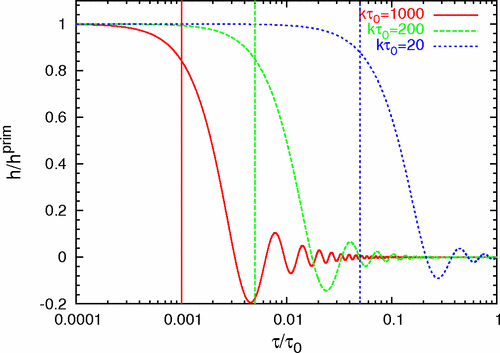
\includegraphics[width=0.7\linewidth, height=0.25\textheight]{Images/Chap3/Watanabe_Komatsu_Fig6}
	\caption{Numerical solutions of tensor perturbations. The solid, dashed, and short-dashed lines show the high, medium, and low frequency modes, respectively. The higher $k$-modes enter the horizon earlier, and are damped more by the cosmological redshift. Vertical lines define the horizon crossing time for each $ k $-mode\cite{Chap3:GW_Watanabe_Komatsu}.}
	\label{fig:watanabekomatsufig6}
\end{figure}

\begin{figure}
	\centering
	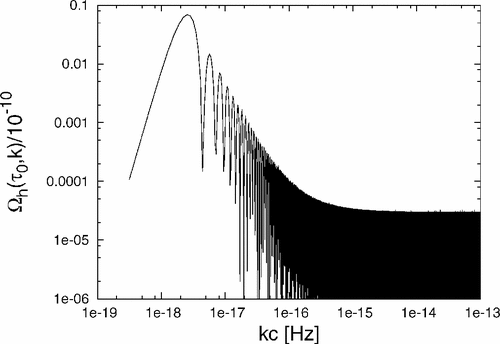
\includegraphics[width=0.7\linewidth, height=0.25\textheight]{Images/Chap3/Watanabe_Komatsu_Fig1}
	\caption{The primordial gravitational wave spectrum at present, $\tau=\tau_{0}$, as a function of the comoving number $ k $. The frequency of the gravitational waves observed today is related to $ k $ by $ f_{0}=kc/2\pi $. In the plot is assumed de-Sitter inflation and then the spectrum at large wavenumber is exactly scale-invariant. In this figure is not taken into account the effects of the change in relativistic degree of freedom or neutrino free-streaming \cite{Chap3:GW_Watanabe_Komatsu}.}
	\label{fig:watanabekomatsufig1}
\end{figure}

In (Fig. \ref{fig:watanabekomatsufig6}, \ref{fig:watanabekomatsufig1}) we report the plots in \cite{Chap3:GW_Watanabe_Komatsu} of the  numerical solution for the temporal evolution of the GW modes and the primordial gravitational wave spectrum at present, respectevely.\\
The first solution (\ref{Chap3:Omega1}) describes $ \Omega_{GW}(\tau,k) $ during radiation era for the modes that entered the horizon before the time at the matter-radiation equality $ \tau_{eq} $. This solution is not relevant for what we observe today. The second (\ref{Chap3:Omega2}) and third (\ref{Chap3:Omega3}) solutions describe $\Omega_{GW}(\tau,k)$ during matter era for the modes that entered the horizon before and after $\tau_{eq}$, respectively. While the expression is slightly complicated, one can find that the second solution is independent of k when the oscillatory part is averaged out, which explains  a scale-invariant spectrum at high frequencies, $ k>k_{eq} \sim 10^{-15} Hz $. On the other hand, the third solution gives $ \Omega_{GW}(\tau,k) \propto k^{-2} $.\\
These arguments can be understood in a more qualitative way and clearly seen in (Fig. \ref{fig:watanabekomatsufig1}). Energy density of gravitational waves evolves just like that of radiation inside the horizon, $ \tilde{\rho_{h}}(\tau,k) \propto a^{-4} $, for $ k\gg aH $. This implies that the relative spectral energy density, $ \Omega_{GW}(\tau,k) $, inside the horizon remains independent of time during the radiation era while it decreases as $ \Omega_{GW}(\tau,k) \propto a^{-1} $ during the matter era. Thus, the modes that entered the horizon during the matter era \textit{later} would decay \textit{less}. As the low frequency modes represent the modes that entered the horizon at late times, $\Omega_{GW}(\tau,k)$ rises toward lower frequencies. On the other hand  $\Omega_{GW}(\tau,k)$ at $  k > 10^{-15} $ is independent of k. These are the modes that entered the horizon  during the radiation era for which $ \Omega_{GW} (\tau,k) $ was independent of time. After the matter-radiation equality all of these modes suffered the same amount of redshift and then the shape of $\Omega_{GW}(\tau,k)$ still remains scale invariant at  $  k > 10^{-15} $.
\section{Thermal history}
In general it is granted that energy density of the universe evolves as $ \rho \propto a^{-4} $ during the radiation era, and this is exactly what caused a scale-invariant spectrum of $ \Omega_{GW}(k) $ at $ k > k_{eq}  $. However, $\rho \propto a^{-4}$ does not always hold in the radiation era because some particles would become non-relativistic before the others and don't contribute anymore to the radiation energy density. Since during the radiation era many kinds of particles interact with photons frequently we can consider thermal equilibrium.\\
We recall that the energy density and the pressure in such era are given by 
\begin{equation}
\label{Chap3:EnergyDensityPressure}
 \rho(T)= \frac{\pi^{2}}{30}g_{*}T^{4} ,  
 \qquad
 p(T)=\frac{1}{3}\rho(T).
\end{equation}	
Moreover, we rewrite the expression for the entropy density,
\begin{equation}
	\label{Chap3:entropy}
	s(T)=\frac{2\pi^{2}}{45}g_{*s}(T)T^{3},
\end{equation}
with $ s(T) =(\rho(T) + p(T))/T $. The effective number of degree of freedom, $ g_{*}(T) $ and $ g_{*s} $, count respectively the (effective) number of relativistic species contributing to the radiation energy density and entropy. In an adiabatic system, the entropy per unit comoving volume must be conserved, i.e. 
\begin{equation}
	\label{Chap3:conservationEntropy}
	S(T) = s(T)a^{3}(T) = constant.
\end{equation}
From the equation for energy density in (\ref{Chap3:EnergyDensityPressure}) we obtain the relation for the temperature
\begin{equation}
\label{Chap3:DependenceTemperature}
T = (30/\pi)^{1/4} \rho^{1/4}g_{*}^{-1/4} 
\end{equation}
and, using (\ref{Chap3:conservationEntropy}),
\begin{equation}
	S(T)=\frac{2\pi^{2}}{45}g_{*s}(T)T^{3}a^{3} = \Big (\frac{2\pi^{2}}{45}\Big)\Big(\frac{30}{\pi}\Big)^{3/4} g_{*s}\ \rho^{3/4}g_{*}^{-3/4}a^{3} = const,
\end{equation}
From which we obtain the beheaviour of the energy density
\begin{equation}
	\label{Chap3:DependenceEnergyDensity}
	\rho \sim g_{*}g_{*s}^{-4/3}a^{-4}.
\end{equation}
We see then, unless $ g_{*} $ and $ g_{*s} $ are independent of time, the evolution of $\rho$ would deviate from $\rho \sim a^{-4}$. In other words, the evolution of $\rho$ during the radiation era is sensitive to how many relativistic species the universe had at a given epoch (Fig. \ref{fig:watanabekomatsufig2}).\\
\begin{figure}
	\centering
	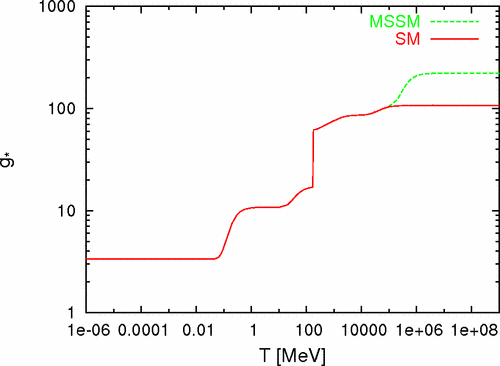
\includegraphics[width=0.7\linewidth, height=0.25\textheight]{Images/Chap3/Watanabe_Komatsu_Fig2}
	\caption{Evolution of the effective number of relativistic degree of freedom contribuiting to energy density, $ g_{*} $, as a function of temperature. The solid and dashed lines represent  $ g_{*} $ in the Standard Model and in the minimal extension of Standard Model (MSSM), respectively. MSSM also includes particles in supersymmetric models. At the energy scales above $ \sim 1$ TeV, $ g_{*}^{SM}=106.75 $ and $ g_{*}^{MSSM} \simeq 220 $. At energy scales below $ \sim 0.1 $ MeV, $ g_{*}\simeq 3.3626 $ and $ g_{*s}=3.9091 $; $ g_{*}=g_{*s} $ otherwise \cite{Chap3:GW_Watanabe_Komatsu}. }
	\label{fig:watanabekomatsufig2}
\end{figure}

We can then understand how $ g_{*} $ and $ g_{*s} $ would affect the shape of $ \Omega_{GW}(\tau_{0},k) $. While energy density of the universe  during the radiation era is affected by $ g_{*} $, $ g_{*s} $ as $ \rho_{cr} \propto g_{*}g_{*s}^{-4/3}a^{-4} $, energy density of the gravitational waves always evolves as $\tilde{\rho_{h}}(\tau,k) \propto a^{-4}$ inside the horizon, $ k \ll aH $, regardless $ g_{*} $ or $ g_{*s} $, because the gravitons are not in thermal equilibrium with other particles. Thus, this difference in the evolution of $ \tilde{\rho_{h}} $ and $ \rho_{cr} $ significantly modifies the spectrum of $ \Omega_{GW}(\tau_{0},k) $ at $ k>k_{eq} $.\\
Consider  a gravitational wave mode with $ k $ which entered the horizon at a given time $ \tau_{hc} < \tau_{eq} $ and temperature, $ T=T_{hc} $, during the radiation era. After the mode entered the horizon the amplitude of this mode would be suppressed by the cosmological redshift. We can then derive, at first approximation, the relative spectral density $\Omega_{GW}(\tau_{0},k > k_{eq}) = \tilde{\rho_{h}}(\tau_{0},k)/\rho_{cr}(\tau_{0})$ today. Since density energy of the gravitational waves is independent of other particles, we can write (the mode $ k $ entered the horizon during the radiation era at $ \tau_{hc} $)
\begin{equation}
 \tilde{\rho_{h}}(\tau_{0},k) =  \tilde{\rho_{h}}(\tau_{hc},k)\Big (\frac{a_{0}}{a_{eq}}\Big)^{-4}\Big (\frac{a_{eq}}{a_{hc}}\Big)^{-4},
\end{equation}
where the subscripts 0 and \textit{eq} denote the present value and the value at the radiation-matter equality, respectively.
Instead, the critical energy density of the universe during the matter era scales as $\sim a^{-3}$, and $ \sim g_{*}g_{*s}^{-4/3}a^{-4} $ during  the radiation era:
\begin{equation}
	\label{Chap3:CriticalDensityEvolution1}
	\rho_{crit}(\tau_{0})=\rho_{crit}(\tau_{eq})\Big(\frac{a_{0}}{a_{eq}}\Big)^{-3},
	\qquad
	\rho_{crit}(\tau_{eq})= \rho_{crit}(\tau_{hc})\Big[\frac{g_{*,0}}{g_{*}(T_{hc})}\Big]\Big [\frac{g_{*s,0}}{g_{*s}(T_{hc})}\Big]^{-4/3}\Big(\frac{a_{eq}}{a_{hc}}\Big)^{-4}
\end{equation}  
Combining these equations in the expression for the relative spectral density of the GWs at present, we obtain
\begin{equation}
	\label{Chap3:SpectralDensityAtPresent}
	\Omega_{GW}(\tau_{0}, k>k_{eq}) = \Omega_{GW}(\tau_{hc},k)\Big[\frac{g_{*s}(T_{hc})}{g_{*s0}}\Big]^{-4/3}\Big [\frac{g_{*}(T_{hc})}{g_{*0}}\Big] (1+z_{eq})^{-1},
\end{equation}
where we have used $ (1+z_{eq})^{-1} = a_{eq}/a_{0} $, with $ z_{eq}=3402 $. This equation helps us to understand how $ g_{*s} $ and $g_{*}$ would affect the beheaviour of $ \Omega_{GW}(\tau_{0},h) $.\\
The mode that entered the horizon earlier experienced larger suppression, as $ g_{*} $ and $ g_{*s} $ would be larger than the modes that entered the horizon later. The modes that entered the horizon during the matter era should not be affected by $ g_{*} $ or $ g_{*s} $, as they do not change during this era. (\ref{Chap3:SpectralDensityAtPresent}) can be obtained analytically also  directly from  the equation for the gravitational waves (\ref{Chap3:eomMasslessDesitter}) exploiting $ a''/a $ during the thermal history of the universe (see \cite{Chap3:GW_Watanabe_Komatsu}). 
In \cite{Chap3:GW_Watanabe_Komatsu} is also reported the full  computation of $ \Omega_{GW}(\tau_{0},k) $ obtained numerically integrating the wave equation together with the numerical data of $ g_{*} $ and $ g_{*s} $. The computation accounts also the effect of free-streaming of relativistic neutrinos which have decoupled from thermal equilibrium at $T < 2 $ Mev, and significantly contributes to damping the amplitude of the gravitational waves.\\
\begin{figure}
	\centering
	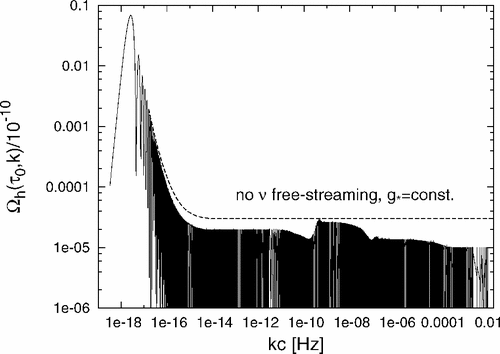
\includegraphics[width=0.7\linewidth, height=0.25\textheight]{Images/Chap3/Watanabe_Komatsu_Fig4}
	\caption{The primordial gravitational wave spectrum at present, $\Omega_{h}(\tau_{0},k)/10^{-10}$, as a function of the comoving wavenumber, $ k $. It is assumed a scale-invariant spectrum and $\Omega_{m}=1-\Omega_{r}, \Omega_{r} = 4.15 \times 10^{-5} h^{-2}, h=0.7$, and $ E_{inf}=10^{16} $ GeV. It is also included the effects of the effective number of relativistic degree of freedom and neutrino free-streaming. The dashed line shows the case in which these effects are ignored \cite{Chap3:GW_Watanabe_Komatsu}.}
	\label{fig:watanabekomatsufig4}
\end{figure}
The effect of evolution of $ g_{*} $ and $ g_{*s} $ can be very important. For example, big changes in  $ g_{*} $ would occur at the electron-positron annihilation epoch ($\sim 0.51$ Mev, $\sim 2 \times 10^{-11}$ Hz), as well as the quark-gluon plasma (QGP) to hadron gas phase  ($\sim 180$ Mev, $\sim 10^{-7}$ Hz). From the analysis comes out that the gravitational wave spectrum is suppressed by roughly $ 20\% $ and $ 30\% $ above the electron-positron annihilation and QGP transition scales, respectively \cite{Chap3:GW_Watanabe_Komatsu}.\\
One may approximately relate the horizon crossing temperature of the universe to the frequency of the gravitational waves.  The horizon crossing mode, $ k_{hc} = a_{hc}H_{hc} $, is related to the temperature at that time by $ H^{2}_{hc}=\frac{8\pi G}{3}\rho_{hc}=\frac{8\pi^{3}G}{90}g_{*,hc}T^{4}_{hc} $. Using entropy conservation $ g_{*s,hc}a^{3}_{hc}T^{3}_{hc} = g_{*s0}a_{0}^{3}T_{0}^{3} $, one can obtain the following conversion factor  from the temperature of the universe to the frequency of gravitational waves observed today \cite{Chap3:Kamionkowsy_Turner},
\begin{equation}
		\label{Chap3:frequencyTodayGW}
		f_{0} = 1.65 \times 2\pi \times 10^{-7} \Big(\frac{T_{hc}}{1 Gev}\Big) \Big [\frac{g_{*s}(T_{hc})}{100}\Big]^{-1/3}  \Big [\frac{g_{*}(T_{hc})}{100}\Big]^{1/2} Hz 
\end{equation}
 which is related to the comoving wavenumber, $ k $ (or $ kc $ in units of Hertz),  by $ 2\pi f_{0} = kc/a_{0} $.\\
 In an extremely high frequency region, $ k_{rh} $, the gravitational wave spectrum should provide us unique informations about the reheating of the universe after inflation. On the other hand, in an extremely low frequency region (below $ \sim 10^{-18}$ Hz ), dark energy dominates the universe and affects the spectrum. The signatures of the primordial gravitational waves may be detected  by CMB polaritation experiments in the low frequency region, $ < 10^{-16} $ Hz. For the higher frequency region, however, direct detection of the gravitational waves would be necessary, and it should allows us to search for a particular cosmological event, such as reheating.
\section{GWs and reheating}
In the previous section we have seen that the spectrum of the inflationary gravitational wave background directly reflects the expansion history of the universe. In particular, we see now that from  the direct detection of  gravitational waves we can extract informations about the reheating epoch, in particular the reheating temperature and the equation of state of the universe after inflation. \\
As discussed, the growing mode solutions to the wave equation (\ref{Chap3:equationGWConformalTime}) have simple qualitative beheaviour: before the mode re-enters the horizon $ h_{\textbf{k}}(\tau) $ is constant. Once the modes cross inside the horizon during the radiation-dominated era the solution is $ h_{\textbf{k}}=h_{prim,\textbf{k}}(j_{0}(k\tau)) $, while for the modes that cross inside the horizon during the matter-dominated era the exact solution is $  h_{\textbf{k}}=h_{prim,\textbf{k}}(3j_{1}(k\tau)/k\tau) $. The Bessel function are given by $ j_{0}(x) = \sin x/x $ and $ j_{1}(x)= \sin x/x^{2} - \cos x/x $.\\
However, well into the matter dominated era the temporal beheaviour of modes that entered the horizon during the radiation-dominated era is also given by $(3j_{1}(k\tau)/k\tau)$.  For example, considering a gravitational wave mode of inflation that re-enters the horizon during the radiation era, its beheaviour is given by
\begin{equation}
\label{Chap3:GWSimpleBeheaviour}
h_{\textbf{k}}(\tau)=h_{\textbf{k}}^{prim}T(k/k_{EQ})\Big (\frac{3j_{1}(k\tau)}{k\tau}\Big),
\end{equation} 
where the transfer function of gravitational wave, $ T(k/k_{EQ}) $, is only a function of $ k/k_{EQ} $, with $ k_{EQ} \equiv a(t_{eq})H (t_{eq}) = 7.1 \times 10^{-2}\Omega_{m}h^{2} $ $ Mpc^{-1} $ \cite{Chap3:GW_Turner_White}.\\
The transfer function has been calculated by integrating (\ref{Chap3:equationGWConformalTime}) numerically from $ \tau=0 $ to $ \tau=\tau_{0} $ and we report the fit in (\ref{TransferFunction}) of \cite{Chap3:GW_Turner_White}, where this approach is introduced. \\
However, as said in the previous section, the effect of the change of the relativistic degree of freedom could be important. Indeed, during the expansion of the universe $ g_{*} $ changes and the expansion rate is modified from simple power law $ a(t) \propto T^{-1} $ during radiation era. This effect yields the damping factor 
\begin{equation}
	\label{Chap3:dampingFactorDOF}
	\Bigg (\frac{g_{*}(T_{in})}{g_{*0}} \Bigg)\Bigg (\frac{g_{*s0}}{g_{*s}(T_{in})}\Bigg)^{4/3}
\end{equation}
on the power spectrum of the gravitational waves, where $ T_{in} $ denotes the temperature at which the corresponding mode enters the horizon, given by \cite{Chap3:ProibingReheatingTemperature2008}
\begin{equation}
	\label{T_{in}}
	T_{in} \simeq 5.8 \times 10^{6}\ Gev\ \Bigg (\frac{g_{*s}(T_{in})}{106.75}\Bigg)^{-1/6} \Bigg (\frac{k}{10^{14}Mpc^{-1}} \Bigg).
\end{equation}
Since we are interested about reheating, we consider the modes that re-enter the horizon during inflation or reheating era. Moreover, we should also include the effect of dark energy that is leading today the expansion of the universe. \\
 Before writing the solution we can rewrite the relative spectral density (\ref{Chap3:relativeSpectralDensity}) as
\begin{equation}
	\label{Chap3:RelativeSpectralDensity2}
	\Omega_{GW}(\tau,k) = \frac{\Delta_{T,prim}^{2}}{12H^{2}(\tau)a^{2}(\tau)}[T'(\tau,k)]^{2} = \frac{1}{12}\Bigg (\frac{k}{aH}\Bigg)^{2}\Delta_{h,prim}^{2}T^{2}_{h}(k).
\end{equation}
The last relation is a good approximation when we consider the modes deep inside the horizon, $ k \ll aH $. It is given by the fact  that the transfer function  is in general given by Bessel type functions, $ T(x) = \frac{1}{x^{n}}[Aj_{n}(x) + By_{n}(x)] $ and its conformal time derivative by $ T'(x) = -\frac{k}{x^{n}}[Aj_{n+1}(x) + By_{n+1}(x)] $, where $ x=k\tau $. Thus, in the limit $ k\ll aH $ we obtain (\ref{Chap3:RelativeSpectralDensity2}) \cite{Chap3:GW_Watanabe_Komatsu}.\\
In a single-field slow-roll inflation the tensor-to-scalar ratio $ r = \Delta_{h,prim}^{2}(k_{0})/\Delta_{\zeta,prim}^{2}(k_{0}) $ can be related to the tilt of the tensor mode spectrum $ n_{T} = d \ln \Delta_{h,prim}^{2}(k_{0})/d \ln k  $ with $ r=-8n_{T} $. From $ r= - 8n_{T} $ we obtain the relation
\begin{equation}
	\label{Chap3:consistencyRelation}
	n_{T}=\frac{d \ln \Delta_{h,prim}^{2}(k)}{d \ln k} = -\frac{r}{8},
\end{equation}
from which
\begin{equation}
	\label{Chap3:ConsistencyRelation2}
	\frac{\Delta_{h,prim}^{2}(k)}{\Delta^{2}_{h,prim}(k_{0})} = \frac{k}{k_{0}}e^{-r/8},
\end{equation}
where $ k_{0} = 0.002 $ Mpc$^{-1}$ is the pivot scale. Thus, we can obtain from the expression of the tensor-to-scalar ratio $ r $ the equation \cite{Chap3:ProspectsForDeterminationWithDetectors}
\begin{equation}
	\label{Chapter3:solutionSpectrumDelta}
	\Delta^{2}_{h,prim}(k) \simeq r\Delta_{\zeta,prim}^{2}(k_{0})\ \exp \Bigg[-\frac{r}{8}\ln \frac{k}{k_{0}} + ... \Bigg].
\end{equation}
The effects of the cosmological evolution after inflation are then all included in the transfer function $ T_{h}(k) $ in (\ref{Chap3:relativeSpectralDensity}) \cite{Chap3:ProspectsForDeterminationWithDetectors}:
\begin{equation}
	\label{Chap3:FinalTransferFunction}
	T^{2}_{h}(k) = \Omega_{m}^{2}\Bigg (\frac{g_{*}(T_{in})}{g_{*0}}\Bigg)\Bigg (\frac{g_{*s}(T_{in})}{g_{*s0}}\Bigg)^{-4/3} \Bigg ( \overline{\frac{3j_{1}(k\tau_{0})}{k\tau_{0}}}\Bigg)^{2} T_{1}^{2}(x_{eq})T^{2}_{2}(x_{R}).
\end{equation}
The subscript 0 denotes the present time and the subscript \textit{in} denotes the time when the mode crosses the horizon. The effective number of degree of freedom at the end of reheating is taken to be the sum of the standard model particles,  $ g_{*}(T_{R}) $ =  $ g_{*s}(T_{R}) = 106.75 $. The values at present are $ g_{*0}=3.36 $ and $ g_{*s0}=3.90 $. $\tau_{0}$ is the present conformal time calculated assuming the universe matter dominated, $ \tau_{0}=2H_{0}^{-1} $. The parameter $\Omega_{m}=\-\Omega_{\Lambda}  $ accounts for the effect of the cosmological constant. In the limit of $ k\tau_{0} \ll 1 $, the spherical Bessel function $ j_{1}(x)=(\sin x -  x\cos x)/x^{2} $ is replaced by $ \overline{j_{1}(k\tau_{0})} \simeq \overline{\cos (k\tau_{0})}/(k\tau_{0}) = 1/(\sqrt{2}k\tau_{0}) $. The first transfer function $ T_{1}(x_{eq}) $  describes the change of the frequency dependence of the spectrum which arises from the change of the expansion rate of the universe at the matter-radiation equality $ t=t_{eq} $
\begin{equation}
	\label{TransferFunction}
	T_{1}^{2}(x_{eq})=[1+1.57 x_{eq} + 3.42 x_{eq}^{2} ],
\end{equation}
where $ x_{eq} = k/k_{eq} $ and $ k_{eq} \equiv \tau_{eq}^{-1} = 7.1 \times 10^{-2} \Omega_{m} h^{2} $ Mpc$^{-1}$. The second transfer function $ T_{2}(x_{R}) $ corresponds to the change of the expansion rate at the end of reheating $ t=t_{R} $ and connects the modes which enter the horizon after and before the reheating ends. \\
Since before the inflaton decays the universe was dominated by the coherent oscillation of the inflaton, the spectrum of the gravitational waves changes for the modes which enter the horizon at the inflaton dominated epoch $ (k>k_{R}) $, where
\begin{equation}
	\label{Chap3:kReheating}
	k_{R}\simeq 1.7 \times 10^{13} Mpc^{-1} \Bigg(\frac{g_{*}(T_{R})}{106.75}\Bigg)^{1/6}\Bigg(\frac{T_{R}}{10^{6}Gev}\Bigg).
\end{equation}
In terms of frequency, this corresponds to 
\begin{equation}
	\label{Chap3:frequencyReheating}
	f_{R} \simeq 0.026\ Hz \Bigg (\frac{g_{*s}(T_{R})}{106.75}\Bigg)^{1/6}\Bigg ( \frac{T_{R}}{10^{6} Gev} \Bigg),
\end{equation}
which is close to the most sensitive frequency of detectors like DECIGO \cite{Chap3:ProibingReheatingTemperature2008}. The transfer function $ T_{2}(x_{R}) $ is obtained  by solving simultaneously the gravitational waves equation and the Friedmann equations taking into account the decay of the inflaton,
\begin{equation}
\ddot{h}_{\lambda,k} + 3H\dot{h}_{\lambda,k} + \frac{k^{2}}{a^{2}}h_{\lambda,k} = 0,
\end{equation}
\begin{equation}
	\dot{\rho_{\phi}} + 3H\rho_{\phi} = -\Gamma_{\phi}\rho_{\phi}
\end{equation}
\begin{equation}
	\dot{\rho_{r}} + 4H\rho_{r} = \Gamma_{\phi}\rho_{\phi},	
\end{equation}
\begin{equation}
	H^{2}=\dfrac{8\pi G}{3}(\rho_{\phi} + \rho_{r}),
\end{equation}
where $\rho_{\phi}$ denotes the energy density of the inflaton coherent oscillation. The best fit of $ T_{2}(x_{R}) $ is given by \cite{Chap3:ProibingReheatingTemperature2008}:
\begin{equation}
	\label{Chap3:TransferFunction2}
	 T_{2}^{2}(x_{R}) = [1-0.32 x_{R} + 0.99 x^{2}_{R}]^{-1},
\end{equation}
where $ x_{R} = k/k_{R} $.\\
$\Omega_{GW}(f)$ beheaves  as $ f^{0} $ for modes which enter the horizon in the radiation era, while it beheaves as $ f^{-2} $ for  modes which enter in the matter era (see later). Since the evolution of inflationary gravitational waves is sensitive to the expansion of the universe, $ H^{-1} $, we obtain a characteristic feature for the modes around $ f \sim f_{R} $. If the universe beheaves like a matter-dominated universe during reheating, the transition from reheating to the radiation domination is seen as a change of the frequency dependence of the spectrum. If this signature exists in the frequency band of direct detection sensitivity, $ 0.1-1 $ Hz, we may able to determine the reheating temperature by measuring the knee-like feature where the frequency dependence changes from $ f^{-2} $ to $ f^{0} $. In this view, $ f_{R} $ is the important frequency where the change of the frequency dependence due to reheating arises. We show the spectra for different values of the reheating temperature in (Fig. \ref{fig:kurojanaginakayamafig1}), where we can see the knee shape around $ f_{R} $.\\
\begin{figure}
	\centering
	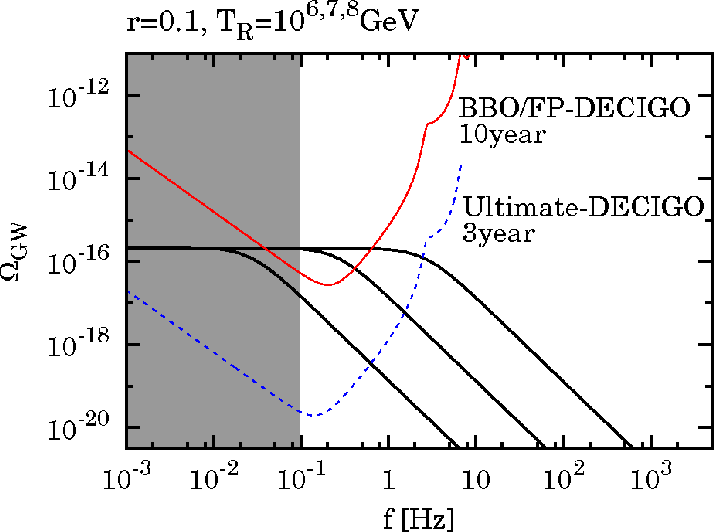
\includegraphics[width=0.7\linewidth, height=0.3\textheight]{Images/Chap3/Kurojanagi_Nakayama_Fig1}
	\caption{The spectra of the inflationary gravitational wave background for different values of the reheating temperature (thick black solid curves with $ T_{R}=10^{6},10^{7},10^{8} $ GeV from left to right). The tensor-to-scalar ratio is taken to be $ r=0.1 $. For reference, it is also plotted the noise spectra for BBO/FP-DECIGO with 10-year observation (red solid) and for Ultimate-DECIGO with 3-year observation (blue-dotted).  The grey  shaded region represents where the noise coming from white dwarf binaries may significantly contribute as systematic error \cite{Chap3:ProspectsForDeterminationWithDetectors}.}
	\label{fig:kurojanaginakayamafig1}
\end{figure}
\begin{figure}
	\centering
	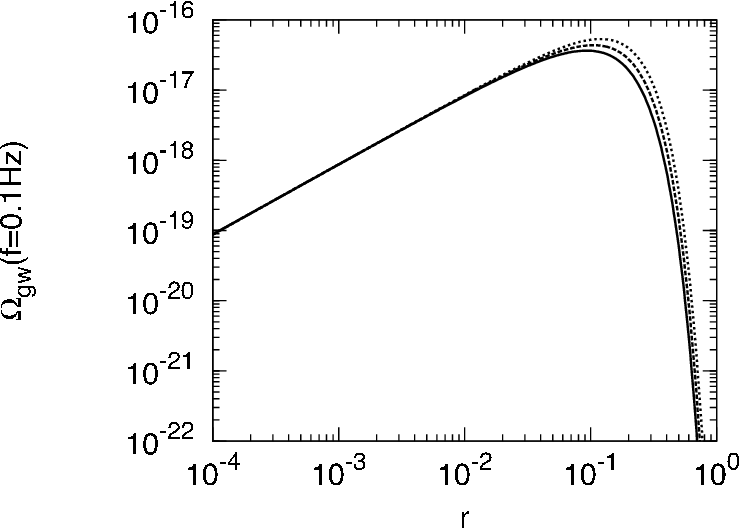
\includegraphics[width=0.7\linewidth, height=0.3\textheight]{Images/Chap3/Nakayama_Saito_Fig2}
	\caption{The spectrum $\Omega_{GW}(f)$ at $ f=0.1 $ Hz for $ \eta=0.01,0,-0.01 $ from upper to lower \cite{Chap3:ProibingReheatingTemperature2008}}.
	\label{fig:nakayamasaitofig2}
\end{figure}
\begin{figure}
	\centering
	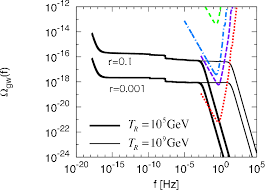
\includegraphics[width=0.7\linewidth, height=0.3\textheight]{Images/Chap3/Nakayama_Saito_Fig3}
	\caption{Primordial gravitational wave spectrum for $ T_{R}=10^{9}$ GeV and $ T_{R}=10^{5}$ GeV are shown by thin and thick lines for $ r=0.1 $ and $ r=0.01 $. Also shown are expected sensitivity of DECIGO (green dashed), correlated analysis of DECIGO (blue-dot dashed), Ultimate-DECIGO (purple dashed) and correlated analysis of ultimate-DECIGO (red dotted), from upper to lower \cite{Chap3:ProibingReheatingTemperature2008}. }
	\label{fig:nakayamasaitofig3}
\end{figure}
We also report in (Fig. \ref{fig:nakayamasaitofig2}) and (Fig. \ref{fig:nakayamasaitofig3}) two plots from \cite{Chap3:ProibingReheatingTemperature2008}. The first plot shows the resulting spectrum $\Omega_{GW}(f)$ at $ f=0.1 $ Hz for the values of the slow-roll parameter $\eta = 0.01, 0, 0.01$ GeV from upper to lower (It is assumed $ T_{R} \le  10^{9}$). The second plot shows the resulting gravitational wave spectrum for $ T_{R}=10^{9} $ GeV and $ 10^{5} $ GeV with $ r=0.1 $ and $ r=0.001 $. \\
Thus, the spectrum of the primordial gravitational waves background generated during inflation crucially depends on the reheating temperature $ T_{R} $.  This fact open the possibility that future experiments devoted to detect gravitational wave background will probe the reheating stage of the universe.\\
The important parameters that determine the primordial gravitational wave spectrum are the tensor-to-scalar ratio $ r $ and the reheating temperature $ T_{R} $. The tensor-to-scalar ratio $ r $ determines the overall normalitation of the spectrum (the amplitude), and $ T_{R} $ fixes the frequency above which the spectrum is significantly suppressed. The important point is that if the knee point in the spectrum  determined by $ T_{R} $ around the frequency $ f_{R} $ lies above the sensitivity of future detectors, $ T_{R} $ can be determined by observation of gravitational waves.\\
The non-zero value of the tensor-to-scalar ratio $ r $ is determined by measurements of the B-mode CMB polaritation  whose detection indirectly confirms the existence of the primordial gravitational wave background. A certain amount of B-modes polaritation has been detected  by BICEP2 collaboration, but its amplitude is compatible with foreground contamination. Current data actually provide only an upper bound on r ($ r_{0.05} < 0.09 $ at $ 95 \% $ C.L.).\\
In \cite{Chap3:ProibingReheatingTemperature2008} and \cite{Chap3:ProspectsForDeterminationWithDetectors} is studied the observable range of $ T_{R} $,  for various value of $ r $, through future mission concepts based on space laser interferometer, like DECIGO \cite{Chap3: DECIGO} and NASA's Big Bang Observer (BBO). DECIGO is a future mission that will explore the gravitational wave range frequency $ 0.1 < f < 10 $ Hz, that would contains important informations about the primordial epoch and likely can put a meaningful constraint on $ T_{R} $ . However, stochastic noise coming from some astrophysical sources must be taken into account for the purpose of detecting gravitational wave background. In particular, gravitational waves from white-dwarf binaries are considered to completely hide the primordial ones for the frequency $ f<0.1 $ Hz. But for the frequency range $ 0.1-10 $ Hz, where DECIGO and BBO are most sensitive, foregrounds from astrophysical sources can be separated. \\
From the analysis of \cite{Chap3:ProibingReheatingTemperature2008} for $ 10^{-3} \le r \le 1 $, direct detection of gravitational wave background can determine the reheating temperature $ T_{R} $, if it lies in the range $ T_{R} \sim 10^{6}-10^{8} $ Gev.\\
On the other hand, in \cite{Chap3:ProspectsForDeterminationWithDetectors} the detectability of $ T_{R} $ is studied using the Fisher information matrix approach. This Fisher matrix is a powerful method used in cosmology to forecast the constraining power of parameter of interest for a given survey.\\
The Fisher matrix  generally depends on the covariance matrix of signals, i.e. the noise properties of the survey configurations. In the case of the stochastic gravitational wave background, direct detection can be attempted by cross-correlating the output signals between detectors. The Fisher matrix $ \mathcal{F}_{ij} $ depends on three ingredients: a total observational time $ T_{obs} $, an overlap reduction function $ \gamma_{ij}(f) $ and the noise spectra $ S_{I}(f) $. These functional form rely on the type of interferometry that we choose. Both DECIGO and BBO are basically designed to aim at the detection of the inflationary gravitational waves with similar frequency ranges around $ 0.1-1 $ Hz. It is chosen a lower cutoff of $ f_{cut}=0.1  $ Hz, below which the signal may be contaminated by noise from cosmological white dwarf binaries. On the other hand, $ f_{max} $ is set to $ f_{max}=\infty $. \\
The Fisher matrix is a product of the signal-to-noise ratios, $ \Omega_{GW}/S $, and the derivative, $ \partial_{p_{i}} \ln \Omega_{GW} $, and hence depends on the parameter response, namely the parameter degeneracy as well as the signal detectability. Fisher matrix can be calculated once the detector parameters are assigned and theoretical predictions for $\Omega_{GW}$ is provided.\\
The marginalized $ 1\sigma $ error is computed with the inverse of the Fisher matrix 
$ \sigma(p_{i}) = \sqrt{(\mathcal{F})^{-1}_{ii}} $. 
We can estimate the detectability of the reheating temperature substituing the expression of the relative spectral density (\ref{Chap3:spectralDensityFinal}) in the Fisher matrix, given by
\begin{equation}
	\label{FisherMatrix}
	\mathcal{F}_{ij}= \Bigg (\frac{3H_{0}^{2}}{10\pi^{2}}\Bigg)^{2}2T_{obs}\sum_{(I,J)}\int_{f_{cut}}^{f_{max}}
	df\frac{|\gamma_{ij}(f)|^{2} \partial_{p_{i}} \Omega_{GW}(f)\partial_{p_{j}}\Omega_{GW}(f)}{f^{6}S_{I}(f)S_{j}(f)}.
\end{equation}
The paramaters  $ r $ and $ T_{R} $ are taken as free and correspond to the amplitude of the spectrum and the frequency of the reheating signature, respectevely. In the plot (Fig. \ref{fig:kurojanaginakayamafig2}) from \cite{Chap3:ProspectsForDeterminationWithDetectors}, is presented an example of future constraints. The fiducial parameters are chosen as $ r = 0.1 $ and $ T_{R}=10^{7} $ Gev. Each ellipse represents the $ 2\sigma $ error contours expected from 1, 3 and 10 years of observation with 	BBO/DECIGO. The error ellipse shrinks more for longer observations due to the fact that the signal-to-noise ratio scales as $\sqrt{T_{obs}}$. \\
\begin{figure}
	\centering
	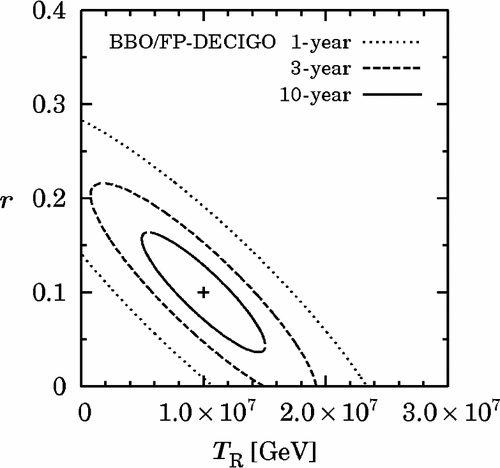
\includegraphics[width=0.7\linewidth, height=0.3\textheight]{Images/Chap3/Kurojanagi_Nakayama_Fig2}
	\caption{The $ 2\sigma $ confidence level contours in the $ T_{R}-r $ plane for 1-year (dotted), 3-year (dashed) and 10-year (solid) observation by BB0/FP-DECIGO. The fiducial parameters are set as $r=0.1$ and $ T_{R}=10^{7} $ GeV, which is shown by a cross mark \cite{Chap3:ProspectsForDeterminationWithDetectors}. }
	\label{fig:kurojanaginakayamafig2}
\end{figure}
\begin{figure}
	\centering
	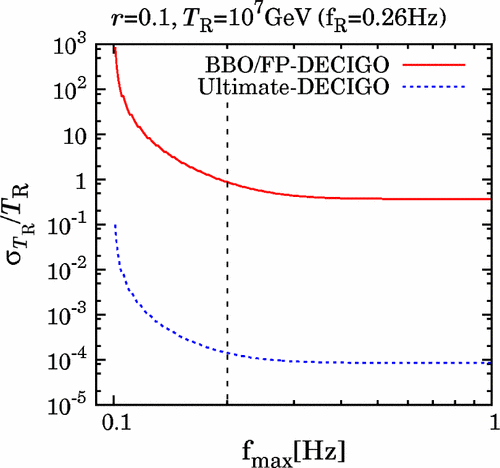
\includegraphics[width=0.7\linewidth, height=0.3\textheight]{Images/Chap3/Kurojanagi_Nakayama_Fig3}
	\caption{The $ 1\sigma $ margnalized errors are shown as a function of $ f_{max} $, calculated assuming $ r=0.1 $ and $ T_{R}=10^{7} $ GeV (corresponding to $ f_{R}=0.26 $ Hz) with 3-year observations. The best sensitivity frequency is plotted as a vertical line \cite{Chap3:ProspectsForDeterminationWithDetectors}.}
	\label{fig:kurojanaginakayamafig3}
\end{figure}
Another interesting question examinated in \cite{Chap3:ProspectsForDeterminationWithDetectors} is what frequency range actually carries information about the reheating temperature i.e. how wide of a band  width is necessary to detect the knee shape with a good accuracy. We report the plot of \cite{Chap3:ProspectsForDeterminationWithDetectors} in (Fig. \ref{fig:kurojanaginakayamafig3}), in which errors in $ T_{R} $ are plotted as a function of the upper frequency limit in the calculation of the Fisher matrix ($ f_{max} $). From the analysis in the paper apparently frequencies above $ f \simeq 0.3$ Hz do not contribute to detection of the reheating temperature. This is because both the suppression of the signal amplitude due to reheating and the increase of the noise spectrum intensity prevents us from reaching the spectrum information.\\
Instead of choosing fixed values of $ r $ and $ T_{R} $ we can discuss the fiducial dependence and predict the parameter space where the signature of reheating can be successfully detected. In (Fig. \ref{fig:kurojanaginakayamafig4}) the marginalized error in $ T_{R}(\sigma_{T_{R}})$							
is calculated by changing $ r $ with the fixed value of $ T_{R}=10^{7} $ Gev. The error becomes smaller as the gravitational wave spectrum is detected with larger signal-to-noise ratio (the spike in the figure is an artificial effect due to the choice of parametrization). Similarly in (Fig. \ref{fig:kurojanaginakayamafig5}) is shown the dependence on the fiducial value of $ T_{R} $ with the fixed value of $ r = 0.1 $. From the plot we can see that the error becomes smaller when the signature of reheating comes into the range of the sensitivity, which corresponds to the reheating temperature of about $ 10^{6} $ Gev to $ 10^{8} $ Gev. The right panel of (\ref{fig:kurojanaginakayamafig5}) shows that Ultimate-DECIGO could determine the reheating temperature with $ 1 \% $ accuracy of $ 1.2 \times 10^{6} $ Gev $ < T_{R} <  3.3 \times 10^{8} $ Gev for $ r=0.1 $, and if $ 2.1 \times 10^{6} $ Gev  $ < T_{R} < 7 \times 10^{7} $ Gev for $ r=0.01 $. We also report in (\ref{fig:kurojanaginakayamafig6}) the parameter space of $ r $ and $ T_{R} $, where the reheating signature is detected at greater than $ 2\sigma $ level ($ T_{R} / \sigma_{T_{R}}  > 2$)  with 3-year observation. It is also shown the parameter region for the detection with a signal-to-noise ratio higher than 5 ($ S/N > 5 $) that is the criterion adopted in \cite{Chap3:ProibingReheatingTemperature2008}. However, in \cite{Chap3:ProibingReheatingTemperature2008} is not taken into account the degeneracy between the parameters $ T_{R} $ and $ r $, given by the fact that as long as the frequency dependence of the spectrum is measured with a good accuracy, we cannot distinguish the spectrum with larger $ T_{R} $ from that with smaller amplitude, i.e. with smaller $ r $. This may cause an underestimate of $ \sigma_{T_{R}} $.
\begin{figure}[]
	\centering
	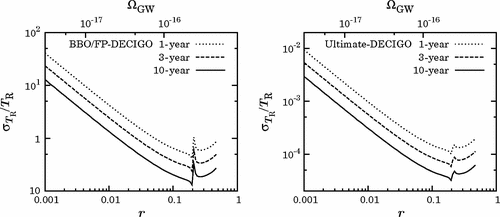
\includegraphics[width=0.8\linewidth, height=0.25\textheight]{Images/Chap3/Kurojanagi_Nakayama_Fig4}
	\caption{The marginalized $ 1\sigma $ uncertainty in $ T_{R} $ as a function $ r $ of BBO/DECIGO (left panel) and Ultimate-DECIGO (right panel). The fiducial value of the reheating temperature is fixed to be $ T_{R}=10^{7} $ GeV. The upper horizontal axis represents the values of $ \Omega_{GW} $ corresponded to $ r $ by (\ref{Chap3:RelativeSpectralDensity2}) \cite{Chap3:ProspectsForDeterminationWithDetectors}. \label{fig:kurojanaginakayamafig4}}
\end{figure}
\begin{figure}[]
	\centering
	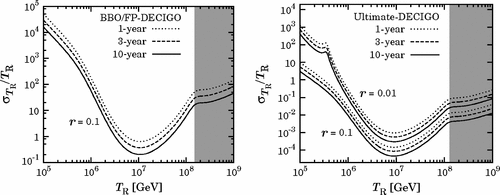
\includegraphics[width=0.8\linewidth, height=0.25\textheight]{Images/Chap3/Kurojanagi_Nakayama_Fig5}
	\caption{The marginalized $ 1\sigma $ uncertainty in $ T_{R} $ as a function of $ T_{R} $ for BBO/DECIGO (left panel) and Ultimate-DECIGO (right panel). The fiducial value of the tensor-to-scalar ratio is fixed to be $ r=0.1 $ \cite{Chap3:ProspectsForDeterminationWithDetectors}.}
	\label{fig:kurojanaginakayamafig5}
\end{figure}
\begin{figure}[]
	\centering
	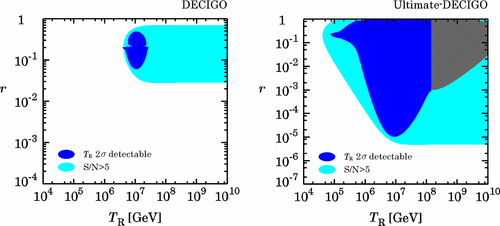
\includegraphics[width=0.8\linewidth, height=0.25\textheight]{Images/Chap3/Kurojanagi_Nakayama_Fig6}
	\caption{$ 2\sigma $ detection of $ T_{R} $ is shown as a blue shaded region for 3-years observations by BBO-FP-DECIGO (left panel) and Ultimate-DECIGO (right panel). The gray area represents the region where $ \sigma_{T_{R}} $ may be underestimated in the previous work \cite{Chap3:ProibingReheatingTemperature2008}, where the Fisher approach was not used. In the light blue shaded region , the inflationary gravitational wave background would be detected with a signal-to-noise ratio higher than 5}
	\label{fig:kurojanaginakayamafig6}
\end{figure}

\section{Late-time entropy production}
So far, we have assumed that there were no late-time entropy production processes after the completion of reheating after inflation. Let us consider also the case in which some other scalar field $\sigma$  dominates the universe some time after the inflaton decays. This new particle eventually decays releasing huge entropy. In some cases, during the radiation-dominated era after the decay of the inflaton, the oscillating $\sigma$ field can dominate over the radiation energy density. Then, the universe enters a matter-dominated like phase due to the $\sigma$ oscillation. After the $\sigma$-field decays into radiation, the universe is dominated by the radiation energy again. Such scenario can be interesting since it diluites all cosmological relics produced in the reheating era. \\
This non-standard cosmological evolution is imprinted in the present gravitational wave spectrum. In the presence of such a late-decaying particle, the additional $\sigma$-matter dominated era suppresses the gravitational wave amplitude for the frequency which re-entered the horizon during or before $\sigma$ begins to dominate the universe \cite{Chap3:ProibingReheatingTemperature2008}. The fitting formula for the transfer function is given by \cite{Chap3:ProibingReheatingTemperature2008}
\begin{equation}
	\label{Chap3:TransferFunctionLateEntropy}
	T^{2}_{h} = \Omega_{m}\Bigg(\frac{g_{*}(T_{in})}{g_{*0}}\Bigg)\Bigg(\frac{g_{*s0}}{g_{*s}(T_{in})}\Bigg)^{4/3}\Bigg (\frac{3j_{1}(k\tau_{0})}{k\tau_{0}}\Bigg)^{2}T_{1}^{2}(x_{eq})T_{2}^{2}(x_{\sigma})T_{3}^{2}(x_{\sigma R})T^{2}_{2}(x_{RF}),
\end{equation}
where $ k_{\sigma} $ corresponds to the wavenumber which enters the horizon at the time  when $\sigma$ decays into radiation after the $\sigma$-dominated era, and it is given by
\begin{equation}
\label{Chap3:kSigma}
k_{\sigma} = 1.7 \times 10^{14} \Big (\frac{g_{*s}(T_{\sigma})}{106.75}\Bigg)^{1/6}\Bigg (\frac{T_{\sigma}}{10^{7} Gev}\Bigg) Mpc^{-1}
\end{equation}
with $ T_{\sigma} $ being the temperature of the universe at the $\sigma$ decay. Before writing down $ k_{\sigma R} $ and $ k_{RF} $ we define the \textit{diluition factor} F, which represents the amount of entropy production by the decay of $\sigma$:
\begin{equation}
	\label{Chap3:DiluitionFactor}
	F \equiv \frac{s(T_{\sigma})a^{3}(T_{\sigma})}{s(T_{R})a^{3}(T_{R})},
\end{equation}
where $ s(T) $ is the entropy density at temperature T. The abundance of all dangerous cosmological relics produced in the reheating era after inflation are diluited by this factor.\\
With this quantity  we can define the other characteristic frequencies as $ k_{\sigma R}=k_{\sigma}F^{2/3} $ and $ k_{RF}=k_{R}F^{-1/3} $. The third transfer function $ T_{3}(x) $ describes the transition from the first radiation-dominated era to the $\sigma$-dominated phase and it is given by \cite{Chap3:ProibingReheatingTemperature2008}
\begin{equation}
	\label{Chap3:ThirdTransferFunction}
	T_{3}(x) = 1 + 0.59x + 0.65x^{2}.
\end{equation}
For the mode $ k_{\sigma R} < k < k_{R}$, which corresponds to the mode which re-enters the horizon in the radiation dominated era before the $\sigma$ domination, the energy density of the gravitational waves is suppressed by the factor $\sim (k_{R}/k_{\sigma R})^{2} = F^{-4/3}$ \cite{Chap3:Seto_Yokohama}. On the other hand there are no effects on large scale with the mode $ k < k_{\sigma} $.\\
The gravitational wave spectrum in the presence of late-time entropy production is then completely characterized by two additional parameters: the diluition factor F and the decay temperature of $\sigma$, $ T_{\sigma} $. Non-negligible effects of $ F $ can affect the overall amplitude of the gravitational wave background for the mode $ k_{\sigma R} < k < k_{R} $ and hence there is a degeneracy between F and the tensor-to-scalar ratio $ r $ when we consider the direct detection around $ 0.1 $ Hz. However, $ r $ should be determined by CMB B-mode measurements. Thus, if future CMB experiments measure $ r $, there does not remain an ambiguity coming from the degeneracy between $ r $ and $ F $. This means that if the result of direct detection experiments deviates from the expected signal from the large scale measurement of $ r $, there must be an entropy production process in the early universe. In (Fig. \ref{fig:nakayamasaitofig6}) is plotted the gravitational wave spectrum with $ F=10^{2} $ and $ F=10^{4} $, and $ r=0.1 $, $ T_{R}=10^{9} $  Gev and $ T_{\sigma} = 1 $ Gev. The figure shows how the gravitational wave spectrum is affected by late-time entropy production.\\
If $ 0.1$ Hz $ < k_{R}(F) <10$ Hz, both $ F $ and $ T_{R} $ can be determined from the shape of the gravitational wave spectrum. In the figure are showned also the future sensitivity to determine the diluition factor $ F $ and the reheating temperature $ T_{R} $ with fixed tensor-to-scalar ratio $ r $, which can be measured by CMB polaritation experiments.
\begin{figure}
	\centering
	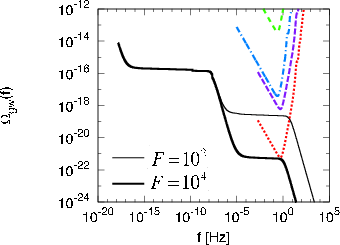
\includegraphics[width=0.7\linewidth, height=0.3\textheight]{Images/Chap3/Nakayama_Saito_Fig6}
	\caption{Gravitational wave spectrum for the diluition factor $ F=10^{2} $ and $ F=10^{4} $. Here is set $ r=0.1, T_{R}=10^{9} $ GeV and $ T_{\sigma}=1 $ GeV. Also shown are expected sensitivity of DECIGO (green dashed), correlated analysis of DECIGO (blue-dot dashed), Ultimate-DECIGO (purple dashed) and correlated analysis of ultimate-DECIGO (red dotted), from upper to lower \cite{Chap3:ProibingReheatingTemperature2008}.}
	\label{fig:nakayamasaitofig6}
\end{figure}

\section{Blue-tilted spectrum}
Although the standard inflation model predicts a red-tilted spectrum since the tensor spectral index $ n_{T} $ has the so-called consistency relation $ n_{T}=-r/8 $, a blue-tilted spectrum can be realized in some non-standard models. There are several observational constraints on the energy density of the stochastic gravitational waves at different frequencies given by pulsar timing, big bang nucleosynthesis (BBN), interferometric GW detectors such as LIGO and VIRGO and so on. Altough these limits are far above the prediction of the standard inflationary models, a strongly blue-tilted tensor spectrum can instead  be detected. Moreover, the mechanism that generate GWs do not necessary  predict a blue-tilted spectrum over all the frequencies. The spectral index of the primordial GW spectrum can change at some frequency. \\
We can use two different approaches to describe GW spectrum. In the first approach we consider constraints on $ n_{T} $ taking into account the suppression of the spectrum at high frequencies due to reheating and late-entropy production, assuming that the primordial spectrum has uniform spectral index over all frequencies. Until now we used this approach considering a fitting formula that can reproduce the effect of the thermal history of the universe on the spectrum with a very good accuracy.\\
In the second approach, introduced in \cite{Chap3:BlueTiltedSpectrum},  we can consider the constraints on $ n_{T} $ without assuming an explicit model of the early universe. Since the shape of the GW spectrum strongly depends on the model assumed, in \cite{Chap3:BlueTiltedSpectrum}
a more general form of the spectrum  is used such that the spectral index changes from $ n_{T} $ to a different value at a given frequency. In this way we can also include the case where the universe is dominated by a component whose equation of state differs from that of radiation/matter component.\\
We first summarize observational bounds on the energy density of the stochastic GWs, which are used to obtain constraints on $ n_{T} $. The constraints adopted are the stringest ones from interferometric GW detectors, pulsar timing array, and BBN. For details and references for this section see \cite{Chap3:BlueTiltedSpectrum}. Here we discuss the main results of the paper.
\subsection*{LIGO + VIRGO}
From interferometric GW detectors such as LIGO, we obtain an upper bound on the stochastic GWs given  by the fact that we don't detect them until now. It is adopted $ 95\% $ C.L. upper bound from the LIGO-Virgo collaboration  \cite{Chap3:Ligo_Virgo}
\begin{equation}
	\label{Chap3:LigoVirgo}
	\Omega_{GW}h^{2} < 2.6 \times 10^{-6} \qquad  [f = 41.5 - 
	169.25\ Hz] 
\end{equation}
where $ h $ is the dimensionless Hubble parameter that parametrizes the present Hubble constant as $ H_{0} = 100h km/s $. The analysis is performed using the approximate form of the GW spectrum, $ \Omega_{GW}(f)=\Omega_{GW,\alpha}(f/100Hz)^{\alpha}, $ where $\alpha$ is the local power index around the sensitive frequency $\sim 100$ Hz, where (\ref{Chap3:LigoVirgo}) is obtained assuming $\alpha=0$.
\subsection*{Pulsar timig array}
 The millisecond pulsars are very precise clocks. Gravitational waves can be searched through the effect of the pulse arrival timings, which currently provides the stringest constraint on the amplitude of GWs at $ f\sim 10^{-8} $ Hz. We can use the bounds obtained by the North American Nanohertz Observatory for Gravitational waves (NANOGrav) project, which gives the upper bound \cite{Chap3:PulsarTiming}
 \begin{equation}
 	\Omega_{GW}h^{2} < 1.1 \times 10^{-8}   \qquad [f = 1/(5.54 years) = 5.72 \times 10^{-9} Hz],
 \end{equation}
where GW spectrum is modeled by $ h_{c}(f) = A_{1year}(f/f_{1year})^{\beta} $, which corresponds to the energy density as $\Omega_{GW}(f)=(2\pi^{2}/3H_{0}^{2})f^{2}h_{c}^{2}(f)$ and $ A_{1year} $ is well approssimated by $ A_{1year}=2.26\times 10^{-14}(5.54year/1year)^{\beta}$.
\subsection*{BBN}
We can also consider contraints from big-bang nucleosynthesis. Primordial GWs contribute to the energy density of the universe as an extra radiation component. Such extra radiation component changes the expansion rate of the universe during BBN and affects the abundance of the light elements. The total energy of GWs, given by integrating the density  parameter  $ \Omega_{GW}(f) $, is therefore constrained not to spoil BBN:
\begin{equation}
	\label{Chap3:ConstraintsBBN}
	\int_{f_1}^{f_2} d(\ln f)\Omega_{GW}(f)h^{2} \le 5.6 \times 10^{-6}(N^{(upper)}_{eff} - 3),
\end{equation}
where $ N^{(upper)}_{eff} $ is the upper bound on the effective number of extra radiation at the time of BBN. The lower limit $ f1 $ is given by the frequency which correspond to the comoving horizon at the time of BBN and $ f_{1}=10^{-10} $ Hz is taken. For the upper cutoff, $ f_{2}=10^{7} $ Hz is taken, which corresponds to the temperature of the universe $ \sim 10^{15} $ Hz. In \cite{Chap3:BlueTiltedSpectrum} is adopted the $ 95 \% $ C.L. upper limit of $ N^{(upper)}_{eff} = 4.65 $.\\
\\
We illustrate how these observational bounds on $\Omega_{GW}$(f) can provide upper bounds to $ n_{T} $ in consideration of the reheating and late-entropy production. Large values of $ n_{T} $ can elude the observational constraints if the reheating temperature is low or the amount of entropy produced at late time is large. We report the result in \cite{Chap3:BlueTiltedSpectrum}. In this paper are investigated constraints on $ n_{T} $ for the cases of the standard reheating and late-time entropy production scenarios and how these constraints depend on the parameters of the two models, in particular $ T_{R} $, $ T_{\sigma} $ and $ F $.
\subsection*{Standard reheating scenario}
In the standard reheating scenario the universe enters in the matter dominated era soon after the end of inflation, and is connected to the radiation dominated era when the temperature of the universe becomes $ T=T_{R} $. In (Fig. \ref{fig:kurojanagitakahashifig3}) are reported the results of \cite{Chap3:BlueTiltedSpectrum}. The plot shows the parameter space ruled out by LIGO, pulsar timing and BBN in the $ n_{T}-T_{R} $ plane. For given $ n_{T} $ and $ T_{R} $ is calculated the stochastic GW spectrum and compared with the observational bounds presented. The GW-spectrum is calculated using the fact that the power spectrum $\Delta_{T}^{2}=\Delta_{T,prim}^{2}(k)T_{T}^{2}(k)$ can be parametrized as
\begin{equation}
\Delta_{T,prim}^{2}(k)=A_{T}(k_{ref})\Big(\frac{k}{k_{ref}}\Big)^{n_{T}},
\end{equation} 
with $ T_{T}(k) $ the transfer function, $ A_{T}(k_{ref}) $ and $ n_{T} $ the amplitude and the spectral index at the reference scale $ k_{ref} $. The amplitude  $ A_{T}(k_{ref}) $  is linked to the tensor-to-scalar ratio $ r $ through $ r(k_{ref})=\Delta_{T,prim}^{2}(k_{ref})/\Delta_{\mathcal{R},prim}^{2}(k_{ref}) $ with $ \Delta_{\mathcal{R},prim}^{2}(k_{ref}) \simeq 2.2 \times 10^{-9} $ the power spectrum for the scalar perturbation at $ k_{ref}=0.01 $ Mpc$ ^{-1} $.\\
Notice that in the case of LIGO and pulsar timing we find a characteristic temperature above which the constraint on $ n_{T} $ does not depend on the reheating temperature. The reason is that the reheating temperature characterizes the frequency of the suppression due to reheating. For a reheating temperature higher than a certain value, the suppression occurs at  frequencies higher than the frequency band of the experiments, and the observational bound on $ n_{T} $ is determined regardless of the effect of reheating. The BBN can put a severe constraint on $ n_{T} $ depending on the reheating temperature because the bound is subject to the integrated value in (\ref{Chap3:ConstraintsBBN}). By putting together all the contraints, we see that the constraint on $ n_{T} $ is relaxed for lower rehating temperatures. Moreover, in order not to spoil the success of BBN we require that the reheating temperature should be larger than about $ 10 $ Mev. This implies that the spectral index $ n_{T} $ should be smaller than $ n_{T}=1.2 $ for $ r=0.2 $.
\begin{figure}
	\centering
	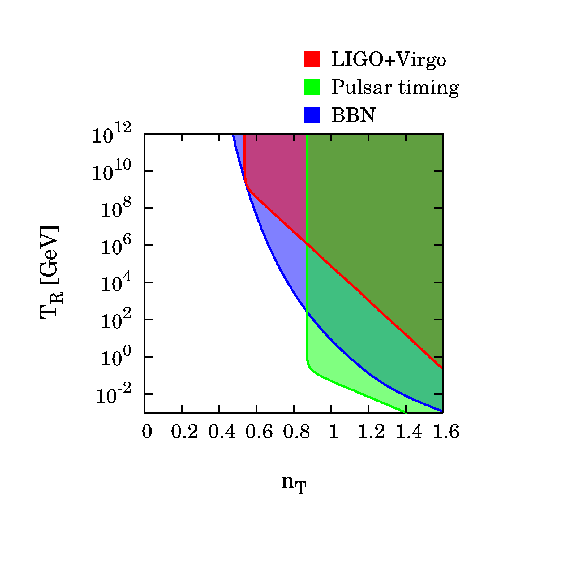
\includegraphics[width=0.7\linewidth, height=0.3\textheight]{Images/Chap3/Kurojanagi_Takahashi_Fig3}
	\caption{$ 2\sigma $ excluded region (colored) in the $ n_{T}-T_{R} $ plane for the case of the standard reheating scenario. The tensor-to-scalar ratio is assumed to be $ r=0.2 $ \cite{Chap3:BlueTiltedSpectrum}.}
	\label{fig:kurojanagitakahashifig3}
\end{figure}
\subsection*{Late-time entropy production}
In the case with late-time entropy production scenario, if large entropy is produced by the decay of another scalar field $\sigma$, the GW spectrum is further suppressed. The degree of suppression depends on the amount of the entropy produced, which is characterized by the diluition factor $ F $. The frequency range of the suppression depends on the temperature of the universe at the end of the second reheating $ T_{\sigma} $. Therefore, the bound on $ n_{T} $ depends on both $ F $ and $ T_{\sigma} $. The reheating temperature $ T_{R} $ is fixed  to be rather high as $ T_{R}=10^{15} $ GeV in order not to include the effect of the first reheating in the constraint on $ n_{T} $ and then simple see the effect of the late-time entropy production. In (Fig. \ref{fig:kurojanagitakahashifig4a}) and (Fig. \ref{fig:kurojanagitakahashifig5a}) are reported the excluded parameter space in the $ n_{T}-F $
 and $ n_{T}-T_{\sigma} $ planes. Since larger values of $ F $ give larger suppression of the GW spectrum, constraints from LIGO and BBN on $ n_{T} $ are weakened as $ F $ becomes large. On the other hand we notice that upper bound on $ n_{T} $ obtained from pulsar timing does not depend on the value of $ F $. This is because the constraint from pulsar timing is put at $ f \sim 10^{-8} $ Hz, which corresponds to the mode who entered the horizon at $ T \sim 1 $ GeV. This involves that for the case of $ T_{\sigma} > 1 $ GeV the spectrum is suppressed at frequencies higher than $ f \sim 10^{-8} $ Hz and then the constraint from pulsar timing is irrelevant to the value of $ F $.\\
Also in this model, $ T_{\sigma} $ determines the frequency of the suppression of the spectrum. However, in contrast to the case of the standard reheating scenario, the suppression due to late-entropy production arises in a certain frequency, which is determined by the amount of entropy production $ F $. Thus, the constraints on $ n_{T} $ from LIGO and BBN do not change depending on the value of $ T_{\sigma} $. The values $ F=10^{2} $ and $ 10^{5} $ assumed here are not enough to reduce the GW amplitude at high frequencies and to relax the observational bounds.\\
 Once the parameters $ T_{\sigma} $, $ F $, $ T_{R} $ and $ r $ are fixed, we can obtain an upper bound on $ n_{T} $ (see \cite{Chap3:BlueTiltedSpectrum}). An interesting fact is that BBN provides a stringest upper bound on $ n_{T} $ in most parameter space because the reheating temperature is assumed to be very high ($ T_{R}=10^{15} $ GeV) and the spectrum is not suppressed by reheating. Then BBN put strong constraints at very high frequency region. Instead, LIGO is sensitive at high frequencies ($\sim 100$ Hz ) and as far as $ T_{\sigma} < 10^{10} $ GeV, the upper bound on $ n_{T} $ depends on the value of F and does not be affected by $ T_{\sigma} $. On the other hand, the pulsar timing has sensitivity at lower frequencies, $ f\sim 10^{-8} $ Hz, and when $ T_{\sigma} $ is below 0.1 GeV the suppression  becomes important at $ f\sim 10^{-8} $ Hz. 
\begin{figure}[h]
	\centering
	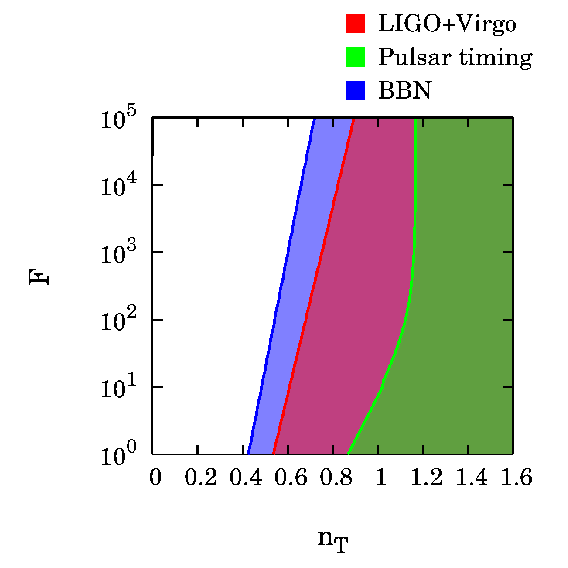
\includegraphics[width=0.45\linewidth, height=0.3\textheight]{Images/Chap3/Kurojanagi_Takahashi_Fig4A}
		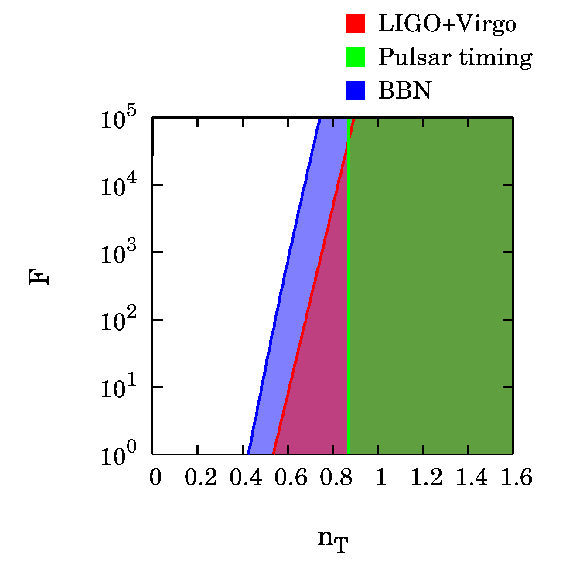
\includegraphics[width=0.45\linewidth, height=0.3\textheight]{Images/Chap3/Kurojanagi_Takahashi_Fig4B}
	\caption{$ 2\sigma $ excluded region (colored) in the $ n_{T}-F $ plane for the cases of $ T_{\sigma}=10^{-2} $ GeV(left) and $ 10^{3} $ GeV (right). We assume $ r=0.2 $ and $ T_{R}=10^{15} $ GeV \cite{Chap3:BlueTiltedSpectrum}. }
	\label{fig:kurojanagitakahashifig4a}
\end{figure}
\begin{figure}[h]
	\centering
	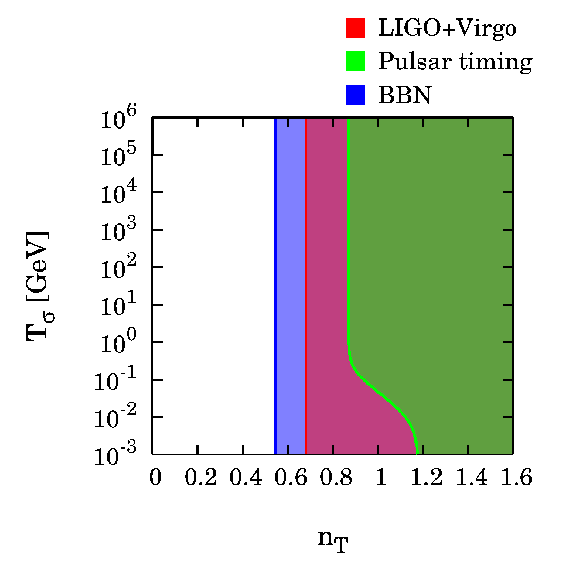
\includegraphics[width=0.45\linewidth, height=0.3\textheight]{Images/Chap3/Kurojanagi_Takahashi_Fig5A}
	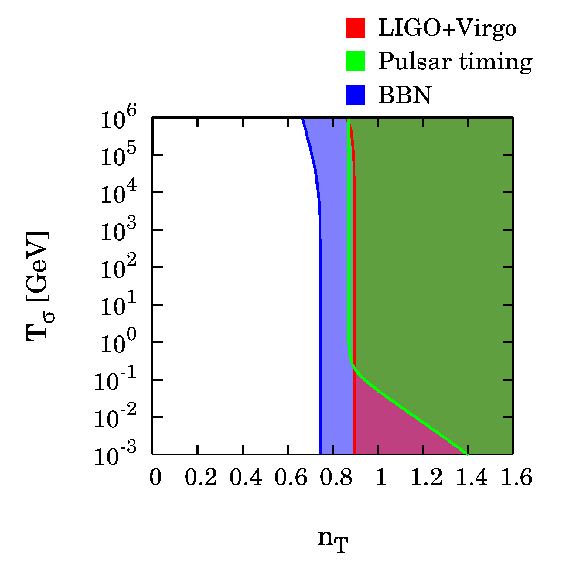
\includegraphics[width=0.45\linewidth, height=0.3\textheight]{Images/Chap3/Kurojanagi_Takahashi_Fig5B}
	\caption{$ 2\sigma $ excluded region (colored) in the $ n_{T}-T_{\sigma} $ plane for the cases of $ F=10^{2} $ GeV (left) and $ 10^{5} $ (right). We assume $ r=0.2 $ and $ T_{R}=10^{15} $ GeV \cite{Chap3:BlueTiltedSpectrum}.}
	\label{fig:kurojanagitakahashifig5a}
\end{figure}
\subsection{Extension to general case}
In the last part of this section we consider the most general case presented in \cite{Chap3:BlueTiltedSpectrum}. The stochastic GW spectrum is modeled by two parameters $\alpha$ and $ f_{\alpha} $, such that the power index of the spectrum changes from $ n_{T} $ to $\alpha$ at a characteristic frequency $ f_{\alpha} $. This approach covers a broad class of models of the early universe. For example, one can interpret the change of the power-law beheaviour as an effect of the change of the background evolution, which is applicable not only for reheating but also for different models. Moreover, we can adjust parameter values to describe particular generation mechanism of primordial GWs which does not predict a uniform spectral index over whole frequency range. \\
The GW spectrum is modelled as 
\
\begin{equation}
	\large
		\label{Chap3:GWExtension}
	\Omega_{GW}(k) = 
	\begin{cases}
		\frac{1}{12}\Big ( \frac{k}{aH} \Big)^{2} T_{T}^{2}(k)A_{T}(k_{ref})\Big (\frac{k}{k_{ref}}\Big)^{n_{T}} \qquad  (k<k_{\alpha})\\		
		\frac{1}{12}\Big (\frac{k}{aH} \Big)^{2} T_{T}^{2}(k)A_{T}(k_{ref})\Big (\frac{k_{\alpha}}{k_{ref}}\Big)^{n_{T}}\Big (\frac{k}{k_{\alpha}}\Big)^{\alpha} \qquad  (k>k_{\alpha})
	\end{cases}
\end{equation}
where $ k_{\alpha} $ is the frequency at which the power index of the spectrum changes from $ n_{T}  $ to $\alpha$. The corresponding frequency is given by $ f_{\alpha}=k_{\alpha}/2\pi $.\\
In this formula $ T_{T}^{2}(k) $ includes only $ T_{1}(k) $ (and not $ T_{2}(k) $ and $ T_{3}(k) $), which means  that only the change of the frequency dependence due to matter-radiation equality is included. The effect of reheating and late-time entropy production is excluded from the transfer function. This allows to treat in a more general way the change of the expansion rate before BBN.\\
An important application of this approach could be in the study of the equation of state during the reheating phase. Assume that the universe is dominated by a fluid whose equation of state parameter is $ \omega $. In the next section we will probe that a gravitational wave which enters the horizon during this phase has a spectral power dependence of
\begin{equation}
	\label{Chap3:OmegaEquationOfState}
	\Omega_{GW} \propto k^{\frac{2(3\omega - 1)}{1+3\omega}}.
\end{equation}
Therefore, when the background equation of state changes from $ \omega $ to $ 1/3 $ (radiation) at the temperature $ T_{\alpha} $, one can describe the GW spectrum by assuming $\alpha$ as 
\begin{equation}
\label{Chap3:dependence}
\alpha = \frac{2(3\omega-1)}{1+3\omega}	+ n_{T},
\end{equation}
and $ f_{\alpha} $ would be the quantity determined by $ T_{\alpha} $.
Moreover, this model can be applied also whenever in some model the spectral index changes from blue-tilted one to another.
This approach could be important when we consider the change of slope of the energy density spectrum of GWs during the reheating epoch.\\
To have an intuitive idea of how the constraint on $ n_{T} $ depends on the value of $ \alpha $ and $ k_{\alpha} (f_{\alpha}) $ we show in (Fig. \ref{fig:kurojanagitakahashifig7}) the plot  in \cite{Chap3:BlueTiltedSpectrum} of the GW spectrum (\ref{Chap3:OmegaEquationOfState}). In the figure three examples of GW spectrum are showned, considering different scenarios of the early universe. First, a blue-tilted spectrum with $ n_{T} = 0.6 $, which underwent the standard reheating scenario with $ T_{R}=10^{6} $ Ge. Next, a scale invariant primordial spectrum in which the kinetic energy of a scalar field dominates the universe. Finally, a primordial spectrum  such that the model predicts a strongly blue-tilted spectrum of $ n_{T}=1 $ around the CMB scale, but at some later stage the situation becomes the same as the standard slow-roll inflation. 
In \cite{Chap3:BlueTiltedSpectrum} are presented also the contour plots in the $ f_{\alpha}-\alpha $ plane for each observational bound (LIGO, pulsar timing, BBN) which represent the upper bound on $ n_{T} $. Thus, once we know an approximated form  of the GW spectrum for some particular model, we can find the values of $\alpha$ and $ f_{\alpha} $ for that model and read off the upper bound on $ n_{T} $ from these plots (see the paper). \\
Thus in this section we have seen a direct application of the reheting temperature.  It is found that the suppression of the GW spectrum due to reheating can significantly relax the constraint on the tensor spectral index $ n_{T} $, depending on the reheating temperature $ T_{R} $. Moreover, taking into account the late-time entropy production, the constraint on $ n_{T} $ changes depending on the amount of the produced entropy $ F $ and the cosmic temperature at the epoch of entropy production $ T_{\sigma} $. For example, assuming $ T_{R}=10^{15}  $ GeV, the constraints on $ n_{T} $ from BBN, LIGO and pulsar timing are $ n_{T} < 0.43,0.54 $ and $ 0.87 $ for $ r=0.2 $ at $ 95 \% $ C.L., respectevely. Assuming $ T_{R}=10^{6} $ GeV, instead, we obtain $ n_{T}<0.64,0.89,0.87 $ from BBN, LIGO and pulsar, respectevely \cite{Chap3:BlueTiltedSpectrum}.\\

\begin{figure}[h]
	\centering
	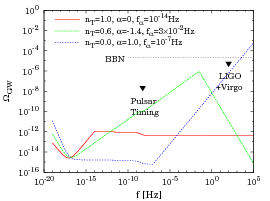
\includegraphics[width=0.7\linewidth, height=0.3\textheight]{Images/Chap3/Kurojanagi_Takahashi_Fig7}
	\caption{GW spectra modeled by $ \alpha $, $ f_{\alpha} $ \cite{Chap3:BlueTiltedSpectrum}.}
	\label{fig:kurojanagitakahashifig7}
\end{figure}

\section{Equation of state}
In the last sections we focused on the determination of the reheating temperature by observing the change of the frequency dependence of the spectrum. On the other hand, direct detection of the inflationary gravitational wave background can be used to determine the equation of state of the early universe at the temperature of $ T \sim  10^{7}$ GeV.\\
In the toy model of reheating showed in the previous chapter we assumed that, after inflation, the inflaton field behaves as non-relativistic matter with equation of state parameter $\omega = 0$. Thus, since this field still dominates the universe in this stage, the universe undergoes a matter-like era. \\
We suppose now, in this model, that the inflaton beheaves during this phase as a generic perfect fluid with equation of state parameter $ \omega_{re} $.
We start rewriting the equation for the radiation during the reheating stage
\begin{equation}
	\label{Chap3:radiationEquation}
	\dot{\rho_{r}} + 4H\rho_{r} = \Gamma_{\phi}\rho_{\phi}.
\end{equation}
Considering the general beheaviour of the scale factor, we can write
\begin{equation}
	\label{Chap3:ScaleFactorBeheaviour}
	\large
	a(t)=a_{osc}\Bigg(\frac{t}{t_{osc}}\Bigg)^{\frac{2}{3(1+\omega_{re})}},
\end{equation}
where $ a_{osc} \equiv a(t_{osc}) $ and $ t_{osc} $ is the time when the inflaton starts to oscillate around the minimum of its potential. During this stage the Hubble rate reads $ H=\frac{\dot{a}}{a}= \frac{2}{3(1+\omega_{re})t} $, and considering $\rho_{\phi} \sim a^{-3(1+\omega_{re})}$, (\ref{Chap3:radiationEquation}) becomes
\begin{equation}
	\label{Chap3:radiationEquationReheating2}
	\dot{\rho_{r}} + \frac{8}{3(1+\omega_{re})t}\rho_{r} = \Gamma_{\phi}\rho_{osc}\Bigg(\frac{a}{a_{osc}}\Bigg)^{-3(1+\omega_{re})},
\end{equation}
with $\rho_{r}(t_{osc})=0$ and $ \rho_{osc} = M^{4} $.
Before $ t \simeq \Gamma_{\phi}^{-1} $ the decay of the inflaton is not efficient. Using (\ref{Chap3:ScaleFactorBeheaviour}) we obtain
\begin{equation}
	\label{Chap3:TimeBeheaviour}
	\Bigg(\frac{a}{a_{osc}}\Bigg)^{-3(1+\omega_{re})} =  \Bigg(\frac{t}{t_{osc}}\Bigg)^{-2},
\end{equation}
and we set $ t_{osc}\simeq M_{pl}/M^{2} $. From (\ref{Chap3:radiationEquationReheating2}), the final equation to solve is
\begin{equation}
	\label{Chap3:FinalEquationRadiationReheating}
		\dot{\rho_{r}} + \frac{8}{3(1+\omega_{re})t}\rho_{r} = \frac{\Gamma_{\phi} M_{pl}^{2}}{t^{2}}.
\end{equation}
We solve this equation in the same way we did for the toy model of reheating. We write the general solution as
\begin{equation}
	\label{Chap3:GeneralSolutionReheating}
	\rho_{r}(t)=e^{-A(t)}\ \int_{t_{osc}}^{t} dt'(g(t')e^{A(t')}),
\end{equation}
where now $ A(t) $ is given by
\begin{equation}
	\label{Chap3:A(t)Parameter}
	A(t)=\frac{8}{3(1+\omega_{re})t},
\end{equation}
and the integral term now reads
\begin{equation}
	\label{Chap3:IntegralTermReheating}
	\int_{t_{osc}}^{t}\ dt' \frac{\Gamma_{\phi} M_{pl}^{2}}{t'^{2}}\Bigg(\frac{t'}{t_{osc}}\Bigg)^{\frac{8}{3(1+\omega_{re})}}=
	\frac{\Gamma_{\phi} M_{pl}^{2}}{t_{osc}^{8/3(1+\omega_{re})}}\int_{t_{osc}}^{t} dt'\ t'^{\frac{2(1-3\omega_{re})}{3(1+\omega_{re})}}.
\end{equation}
Solving the integral and putting all together in (\ref{Chap3:GeneralSolutionReheating}), we finally obtain
\begin{equation}
	\label{Chap3:radiationFinalSolutionTime}
	\rho_{r}(t)=\frac{\Gamma_{\phi}M_{pl}^{2}}{t}\Bigg(\frac{3(1+\omega_{re})}{5-3\omega_{re}}\Bigg)\Bigg(1-\Bigg(\frac{t}{t_{osc}}\Bigg)^{-\frac{5-3\omega_{re}}{3(1+\omega_{re})}}\Bigg).
\end{equation}
At $ t\simeq \Gamma_{\phi}^{-1} $ the decay becomes very efficient and we assume that the radiation era starts immediately. Equating the expression for the radiation density energy and (\ref{Chap3:radiationFinalSolutionTime}) at $ t \simeq \Gamma_{\phi}^{-1} $, we obtain an equation for the reheating temperature:
\begin{equation}
	\label{Chap3:EquatingRadiationThermalitation}
\rho_{rad}=g_{*}\frac{\pi^{2}}{30}T_{reh}^{4}=\Gamma_{\phi}^{2}M_{pl}^{2}\Bigg(\frac{3(1+\omega_{re})}{5-3\omega_{re}}\Bigg),
\end{equation}
that yields
\begin{equation}
	T_{reh} \simeq 1.32\ g_{*}^{-1/4} (\Gamma_{\phi}M_{pl})^{1/2}\Bigg(\frac{3(1+\omega_{re})}{5-3\omega_{re}}\Bigg)^{1/4}.
\end{equation}
Thus, the reheating temperature has a dependence from the equation of state during reheating.\\
In general the equation of state is parametrized by a function $\omega_{re}(t)$ for the universe during the various stages of reheating. When inflation ends, $\omega_{re} = -1/3$. Assuming a massive inflaton, the equation of state climbs to 0. During this initial stage of reheating the frequency of oscillations, characterized by the inflaton mass, will be larger than the expansion rate. As the inflaton decays, the decay products compose an increasing percentage of the energy density of the universe,  increasing the equation of state parameter from 0 to 1/3 at the start of radiation dominance. However, it is estimated that during preheating (the initial stage of reheating) we have an increase of $ \omega_{re} $ from 0 to $\omega_{re} \sim 0.2-0.3$ \cite{Chap3:Podolsky_Felder}. However, the duration of this stage can be considered instantaneous in comparison with the remaining stages of reheating. Thus, in general $ \omega_{re} $ may be rightfully treated as a constant throughout the entire reheating era \cite{Chap3:Cook}.
\subsection{GWs and equation of state}
We can relate the equation of state parameter $\omega$ to the tilt of the gravitational wave background spectrum. We assume that the initial power spectrum has no tilt, i.e. $ \Delta_{h,prim}^{2} \propto k^{0} $. Then, with this assumption the frequency dependence of the spectrum is determined only by the transfer function. Therefore, from (\ref{Chap3:RelativeSpectralDensity2}) we have $\Omega_{GW} \propto k^{2}T^{2}_{T}(k)$.  A gravitational wave, with  initial amplitude of $ h_{\textbf{k},prim} $, mantains constant amplitude outside the horizon and it starts to decrease inversely proportional to the scale factor when the mode re-enters the horizon. Then, we can rewrite the transfer function as $ T_{T}(k) = |h_{\textbf{k,0}}|/|h_{\textbf{k},prim}| = (a_{0}/a_{in})^{-1} $, that implies $ \Omega_{GW} \sim k^{2}a^{2}_{in} $. We know that a mode re-enters the horizon  when $ k = aH $. Considering that the Hubble rate is given in terms of the equation of state as $ H^{2} \propto a^{-3(1+\omega)} $, we obtain $ a_{in} \propto k^{-2/(1+3\omega)} $. Thus, for modes which enter the horizon when the universe has the equation of state $\omega$, the spectrum has the frequency dependence of
\begin{equation}
	\label{Chap3:SpectrumFrequencyDependence}
	\Omega_{GW} \propto k^{\frac{2(3\omega - 1)}{3\omega + 1}}.
\end{equation} 
If we parametrize  the amplitude of the gravitational wave background spectrum, normalizing at $ f=F $, it reads
\begin{equation}
	\label{Chap3:SpectrumFrequencyDependenceParametrization}
	\Omega_{GW}(f) = \Omega_{GW,F}(f/F)^{\frac{2(3\omega - 1)}{3\omega + 1}}.
\end{equation}
Thus, from this equation we can easily see the change of slope of the spectrum at the reheating temperature in the case of the transition from the matter-like era after inflation to radiation era. Indeed, matter-dominated era ($ \omega=0 $) and radiation-dominated era ($\omega=1/3$) corresponds to the frequency dependence $ f^{-2} $, $ f^{0} $, respectevely \cite{Chap3:ProspectsForDeterminationWithDetectors}. \\
From the analysis of \cite{Chap3:ProspectsForDeterminationWithDetectors} results that the value of the tilt is more sensitive to the change of $\omega$ when the fiducial model is $ \omega \sim 0 $ than when $\omega$ has larger value. Then it is easier for direct detection experiments  distinguish the model with smaller value of $\omega$.
\section{Informations from CMB}
Another possibility for extracting information about reheating is to consider the expansion history of the universe between the time the observable CMB scales crossed outside the Hubble radius during inflation and the time they later re-entered. We can start by recapping the cosmic expansion history.\\
At early times, the inflaton field $\phi$ drives the quasi-de-Sitter stage for $ N_{k} $ e-folds of expansion and the reheating comoving horizon scale decreases as $ \sim a^{-1} $. The reheating phase starts when the accelerated expansion ends and the comoving horizon starts to increase. After another $ N_{re} $ e-folds of expansion, the energy in the inflaton field has been completely dissipated into a hot plasma with a reheating temperature $ T_{re} $. After that, the universe expands under radiation domination for another $ N_{RD} $ e-folds, before it makes the transition to the matter-dominated era. Thus, the number of e-folds between the time that the current comoving horizon scale exited the horizon during inflation and the end of inflation must be related to the number of e-folds between the end of inflation and today. Then, studying the expansion history of the universe we can trace the diluition of the energy density (Fig. \ref{fig:daikamionkowsifig1}) \cite{Chap3:Kai_Kamionkowsy}. \\
\begin{figure}
	\centering
	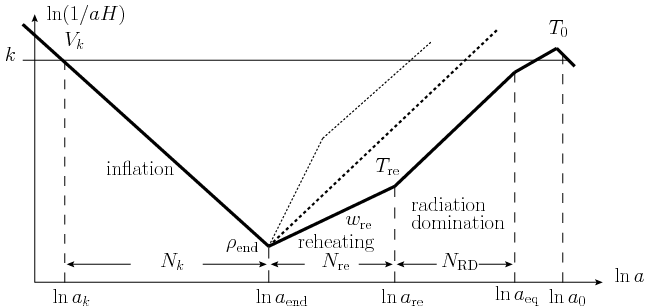
\includegraphics[width=0.8\linewidth, height=0.3\textheight]{Images/Chap3/Dai_Kamionkowsi_Fig1}
	\caption{The evolution of the comoving Hubble scale $ 1/aH $. The reheating phase connects the inflationary phase and the radiation era. Compared to instantaneous reheating (thick dotted curve), a reheating equation of state parameter $ \omega_{re}<1/3 $ implies more post-inflationary e-folds of expansion. Fewer post-inflationary e-folds requires $ \omega_{re} > 1/3 $ (thin dotted curve) \cite{Chap3:Kai_Kamionkowsy}.}
	\label{fig:daikamionkowsifig1}
\end{figure}
In this section we want find a connection between the CMB contraints on the primordial power spectrum (which would correspond to a prediction for $ N_{k} $) for a given inflationary model, and reheating parameters such as $ N_{re} $ (the duration of reheating). Moreover, for a given single-field inflationary model and for a given equation of state during reheating, we may use the CMB data to place constraints on the reheating temperature. We derive expression for the reheating parameters $ (N_{re}$,$T_{re}$ and $ \omega_{re} $) in terms of a set of physical quantities that are specific to inflation and to the cosmological evolution subsequent to reheating (for reference see \cite{Chap3:Cook} and \cite{Chap3:Kai_Kamionkowsy}).\\
 Consider a single-field inflationary model with background field equation $ \ddot{\phi}+3H\dot{\phi} + V'=0 $. First, we derive an expression for $ N_{re} $. Assuming a constant equation of state during reheating  the density energy of the universe beheaves as $ \rho \sim a^{-3(1+\omega_{re})} $. We write
\begin{equation}
	\label{Chap3:DensityEnergyBeheaviour}
	\frac{\rho_{end}}{\rho_{re}}=\Bigg( \frac{a_{end}}{a_{re}}\Bigg)^{-3(1+\omega_{re})},
\end{equation}
where the subscripts \textit{end} and \textit{re} denotes, respectevely, the end of inflation and the end of reheating. In terms of e-foldings, $ N_{re}=ln(a_{re}/a_{end}) $, we obtain
\begin{equation}
	\label{Chap3:Nre}
	N_{re}=\frac{1}{3(1+\omega_{re})}\ln\Bigg(\frac{\rho_{end}}{\rho_{re}}\Bigg).
\end{equation}
For example,  consider for the inflaton power-law potentials
\begin{equation}
	\label{Chap3:potentialInflation}
	V(\phi)=\frac{1}{2}m^{4-\alpha}\phi^{\alpha},
\end{equation}
with power-law $\alpha$ and mass parameter $ m $. We can determine the number of e-folds $ N_{k} $ from the time that the field value is $\phi_{k}$ until the end of inflation $ \phi_{end} $: 
\begin{equation}
	\label{Chap3:N_{k}}
	N_{k}=\int_{t_{k}}^{t_{end}} H dt = \int_{\phi_{k}}^{\phi_{end}}\frac{H}{\dot{\phi}}d\phi.
\end{equation}
Using the equation of motion  $\dot{\phi} \simeq -V'(\phi)/3H $, and $ H^{2}\simeq (8\pi /3M_{pl}^{2})V(\phi) $ during inflation, we obtain
\begin{equation}
	\label{Chap3:eFolds}
	N_{k}=-\int_{\phi_{k}}^{\phi_{end}}\Bigg(\frac{8\pi \phi}{M_{pl}^{2}\alpha}\Bigg)d\phi = \frac{\phi^{2}_{k} - \phi^{2}_{end}}{2\alpha M_{pl}^{2}} \simeq \frac{\phi_{k}^{2}}{2\alpha M_{pl}^{2}},
\end{equation}
where we have assumed that the field value at the end of inflation $\phi_{end}$ is small compared to that during the slow-roll. \\
For this model we can find also a simple relation for the slow-roll parameters
\begin{equation}
	\label{Chap3:slowRollParameters}
	\epsilon \simeq \frac{M_{pl}^{2}}{2}\Bigg(\frac{V'(\phi)}{V(\phi)}\Bigg)^{2},
	\qquad
	\eta \simeq M_{pl}^{2}\Bigg(\frac{V''}{V}\Bigg).
\end{equation}
Using the relation (\ref{Chap3:eFolds}), the slow-roll parameters can be simply rewritten in this model as
\begin{equation}
	\label{Chap3:slowRollParameters2}
	\epsilon_{k} = \frac{\alpha}{4N_{k}}
	\qquad
	\eta_{k}=\frac{\alpha-1}{2N_{k}},
\end{equation}
where they are evaluated at the reference scale $ k $. Finally, we obtain a simple relation also for the spectral tilt at the scale $ k $:
\begin{equation}
	\label{Chap3:spectralTilt}
	n_{s}-1=-6\epsilon + 2\eta = -\frac{\alpha + 2}{2N_{k}}.
\end{equation}
In cosmology we observe perturbation modes on scales that are comparable to that of the horizon. For reference scale we choose the pivot scale at which Planck determines $ n_{s} $, $ k=0.05 $ Mpc$ ^{-1} $. The comoving Hubble scale $ a_{k}H_{k}=k $ when this mode exited the horizon can be related to that of the present time by means
\begin{equation}
\label{Chap3:relationBetweenScales}
\frac{k}{a_{0}H_{0}} = \frac{a_{k}}{a_{end}}\frac{a_{end}}{a_{re}}\frac{a_{re}}{a_{eq}}\frac{a_{eq}H_{eq}}{a_{0}H_{0}}\frac{H_{k}}{H_{eq}},
\end{equation} 
where quantities with subscript k are evaluated at the time of the horizon exit. Same thing for the other subscripts: end of inflation (end), end of reheating (re), radiation-matter equality (eq) and the present time (0). Then we use $ e^{N_{k}}=a_{end}/a_{k},\ e^{N_{re}}=a_{re}/a_{end}  $ and $ e^{N_{RD}}=a_{eq}/a_{re} $ to obtain a constraint on the total amount of expansion,
\begin{equation}
	\label{Chap3:relationBetweenScales2}
	\ln \Bigg(\frac{k}{a_{0}H_{0}}\Bigg) = -N_{k} - N_{re} - N_{RD} + \ln \Bigg(\frac{a_{eq}H_{eq}}{a_{0}H_{0}}\Bigg) + \ln \Bigg(\frac{H_{k}}{H_{eq}}\Bigg).   
\end{equation}
To solve this equation we first  write an expression for $ H_{k} $ as a function of $ n_{s} $. Using the definition of the tensor-to-scalar ratio $ r= P_{h}/P_{\zeta} $, with $ P_{h}=(2H^{2})/(\pi^{2}M_{pl}^{2}) $ and $ P_{\zeta} = A_{s} $ at the pivot scale 
\begin{equation}
\label{chap3:tensortToScalarRatio}
r_{k}=\frac{2H^{2}_{k}}{\pi^{2}M_{pl}^{2}A_{s}}.
\end{equation}
Using the consistency relation $ r=16\epsilon $ we obtain
\begin{equation}
	H_{k}\simeq \pi M_{pl}\sqrt{8A_{s}\epsilon_{k}}.
\end{equation}
We can then express $ H_{k} $ in terms of the spectral tilt $ n_{s} $, the power-law index $\alpha$, and $ A_{s} $, using (\ref{Chap3:spectralTilt}) and (\ref{Chap3:slowRollParameters2}). The expression for $ H_{k} $ becomes
\begin{equation}
	\label{chap3:expressionHk}
	H_{k}=\pi M_{pl}\sqrt{\frac{2A_{s}\alpha (1-n_{s})}{\alpha +2}}.
\end{equation}
The energy density at the end of reheating determines the reheating temperature through $\rho_{re}=(\pi^{2}/30)g_{re}T^{4}_{re}$. The subsequent expansion is mainly driven by hot radiation, except for very recently non-relativistic matter and dark energy. Thus, for semplicity we assume that no immense entropy production occurs after $ T_{re} $. Under this assumption, the reheating entropy is preserved in the CMB-neutrino background today, and leads to the relation
\begin{equation}
	\label{Chap3:relationEntropy}
	g_{s,re}T_{re}^{3}a_{re}^{3}=g_{0s}T_{0}^{3}a_{0}^{3},
\end{equation}
from which
\begin{equation}
	\label{Chap3:relationEntropy2}
	g_{s,re}T_{re}^{3} = \Bigg(\frac{a_{0}}{a_{re}}\Bigg)^{3}\big(2T_{0}^{3} + 6 \cdot \frac{7}{8} \cdot T_{\nu 0}^{3}\big),
\end{equation}
where $ T_{0}=2.725  $ K is the present CMB temperature, and $ T_{\nu,0}=(4/11)^{1/3}\ T_{0} $ is the neutrino temperature. $ g_{re} $ is the effective number of degree of freedom at the end of reheating. From  (\ref{Chap3:relationEntropy2}) we can derive a relation between  today CMB-temperature $ T_{0} $ and the reheating temperature $ T_{re} $:
\begin{equation}
\label{Chap3:RelationReheatingToday}
\frac{T_{re}}{T_{0}}=\Bigg(\frac{43}{11g_{s,re}}\Bigg)^{1/3}\frac{a_{0}}{a_{eq}}\frac{a_{eq}}{a_{re}}.
\end{equation}
Using $ e^{-N_{RD}} = a_{re}/a_{eq}$, we rewrite the reheating temperature as
\begin{equation}
\label{Chap3:ReheatingTemperature}
T_{re} = T_{0}\Bigg(\frac{43}{11 g_{s,re}}\Bigg)^{1/3}\Bigg(\frac{a_{0}}{a_{eq}}\Bigg)e^{N_{RD}}.
\end{equation}
We also rewrite $ a_{0}/a_{eq} $ using (\ref{Chap3:relationBetweenScales}),
\begin{equation}
\label{Chap3:a0/aeq}
\frac{a_{0}}{a_{eq}}= \frac{a_{0}H_{0}}{k}\frac{a_{k}}{a_{end}}\frac{a_{end}}{a_{re}}\frac{a_{re}}{a_{eq}}\frac{H_{eq}}{H_{0}}\frac{H_{k}}{H_{eq}},
\end{equation}
that leads
\begin{equation}
\frac{a_{0}}{a_{eq}}= \frac{a_{0}H_{k}}{k}e^{-N_{k}}e^{-N_{re}}e^{-N_{RD}}.
\end{equation}
With this expression for $ a_{0}/a_{eq} $ we can finally rewrite the reheating temperature as
\begin{equation}
	\label{Chap3:reheatingTemperature3}
	T_{re} = T_{0}\Bigg(\frac{43}{11 g_{s,re}}\Bigg)^{1/3}\Bigg( \frac{a_{0}H_{k}}{k} \Bigg)e^{-N_{k}}e^{-N_{re}}.
\end{equation}
From this relation we see that larger values of $ N_{re} $ corresponds to smaller $ T_{re} $ and viceversa. In other words, quicker and more efficiently reheating takes place, larger becomes the reheating temperature. \\
We use now the fact that at the end of inflation the equation of state has to be $ \omega_{end}=-1/3 $ to stop the exponential quasi-de-Sitter expansion ($\omega_{inf} \simeq -1$). At this time then we have that the energy density and the pressure of the inflaton read
\begin{equation}
	\rho_{end} = \frac{1}{2}\dot{\phi^{2}} + V_{end}(\phi),
	\qquad
	P_{end}=  \frac{1}{2}\dot{\phi^{2}} - V_{end}(\phi),
\end{equation}
with the equation of state $ P_{end}=\omega_{end}\ \rho_{end}=-(1/3)\rho_{end} $, and the inflaton potential evaluated at the end of inflation. Using the equation of state at the end of inflation and  these expressions, we obtain 
$ -\frac{1}{3}\rho_{end}= \frac{1}{2}\dot{\phi^{2}}-V_{end} $. Using also $ \frac{1}{2}\dot{\phi^{2}}=\rho_{end}-V_{end} $, we obtain the simple relation 
\begin{equation}
	\label{Chap3:energyDensityPressure}
	\rho_{end}=\frac{3}{2}V_{end}.
\end{equation}
Plugging this into $ N_{re}=\frac{1}{3(1+\omega_{re})}\ln(\rho_{end}/\rho_{re})$, $ N_{re} $ becomes
\begin{equation}
\label{Chap3:Nre2}
N_{re}=\dfrac{1}{3(1+\omega_{re})}\ln \Bigg(\frac{3 V_{end}}{2\rho_{re}} \Bigg) = \dfrac{1}{3(1+\omega_{re})}\ln \Bigg( \frac{30 \cdot \frac{3}{2} V_{end}}{\pi^{2}g_{re}T^{4}_{re}}\Bigg).
\end{equation}
Finally, using the expression found for the reheating temperature (\ref{Chap3:reheatingTemperature3}), it reads
\begin{equation}
\label{Nre3}
N_{re}=\frac{4}{3(1+\omega_{re})}\Bigg[  \frac{1}{4} \ln \Bigg(\frac{45}{\pi^{2} g_{re}}\Bigg)   + \ln \Bigg(\frac{V_{end}^{1/4}}{H_{k}}\Bigg) +  \frac{1}{3}\ln \Bigg(\frac{11 g_{re}}{43}\Bigg) + \ln \Bigg(\frac{k}{a_{0}T_{0}}\Bigg) + N_{k} + N_{re}    \Bigg].
\end{equation}
Solving this in terms of $ N_{re} $, assuming $ \omega_{re} \ne 1/3 $, we find
\begin{equation}
	\label{Chap3:Nre3}
	N_{re}=\frac{4}{3(1-\omega_{re})}\Bigg[ - \frac{1}{4} \ln \Bigg(\frac{45}{\pi^{2} g_{re}}\Bigg)   - \ln \Bigg(\frac{V_{end}^{1/4}}{H_{k}}\Bigg) -  \frac{1}{3}\ln \Bigg(\frac{11 g_{re}}{43}\Bigg) - \ln \Bigg(\frac{k}{a_{0}T_{0}}\Bigg) - N_{k}     \Bigg].
\end{equation}
The second and the last terms in the right part of this equation depend on the specific inflationary model, since $ V_{end} $ is the potential of the inflaton evaluated at the end of inflation, and $ N_{k} $ is the number of e-foldings between the pivot scale $ k $ crosses outside the Hubble radius and the time when inflation ends. Assuming $ g_{re} \simeq 100 $ and using Planck's pivot scale of $ 0.05 $ Mpc$^{-1}$, one obtains a simplified expression for $ N_{re} $, without specifying a particular inflationary model:
\begin{equation}
	\label{Chap3:NreFinalForm}
	N_{re}=\frac{4}{(1-3\omega_{re})}\Bigg[61.6 - \ln \Bigg( \frac{V_{end}^{1/4}}{H_{k}}\Bigg) - N_{k}     \Bigg].
\end{equation}
Moreover, plugging this equation into (\ref{Chap3:reheatingTemperature3}) we can find another expression for the reheating temperature,
\begin{equation}	
T_{re} = \Bigg[\Bigg(\frac{43}{11g_{re}}\Bigg)^{1/3}\frac{a_{0}T_{0}}{k}H_{k}e^{-N_{k}}\Big[\dfrac{45 V_{end}}{\pi^{2}g_{re}}\Big]^{-\frac{1}{3(1+\omega_{re})}}\Bigg]^{\frac{3(1+\omega_{re})}{3\omega_{re}-1}}.	
\end{equation}
The results obtained for $ N_{re} $ in (\ref{Chap3:NreFinalForm}) and (\ref{Chap3:Nre3}) are valid only if $\omega_{re} \ne 1/3$. Indeed, if $\omega_{re}=1/3$ in  (\ref{Chap3:Nre3}), $ N_{re} $ cancels from both sides of the equation. Assuming $ g_{re} = 100 $, and Planck's pivot scale, one finds \cite{Chap3:Cook}
\begin{equation}
	61.6 = \ln \Bigg( \frac{V_{end}^{1/4}}{H_{k}}\Bigg) + N_{k}.
\end{equation}
The issue is that we are defining the start of radiation dominance as the moment in which $\omega_{re}=1/3$. If $\omega_{re}$ is already equal to $ 1/3 $ during the reheating phase, then there is ambiguity in differentiating the two regimes. This implies that for $\omega_{re}=1/3$ is not possible to derive a prediction for $ N_{re} $ or $ T_{re} $ but, instead, for a particular inflation model, one finds a prediction for $ n_{s} $.\\
Going back to the inflaton potential $ V(\phi)=\frac{1}{2}m^{4-\alpha}\phi^{\alpha} $, we have found the expression for $ N_{k}=\frac{\alpha + 2 }{2(1-n_{s})} $, $ H_{k}=\pi M_{pl}\big(\frac{4\pi A_{s}(1-n_{s})}{\alpha +2}\big)^{1/2} $ in terms of $\alpha$, $ n_{s} $ and $ A_{s} $.\\
 We finally compute also $ V_{end} $ in terms of $ n_{s} $ and $ A_{s} $. To find $ V_{end} $ we start from the expression for $ H_{k} $ in terms of the potential
 \begin{equation}
\label{Chap3:HubblekPotential}
H_{k}\simeq  \frac{8\pi}{3M_{pl}^{2}}V(\phi_{k})= \frac{8\pi}{3M_{pl}^{2}}\frac{1}{2}m^{4-\alpha}\phi_{k}^{\alpha}
 \end{equation}
from which $ m^{4-\alpha} \simeq \frac{6M_{pl}^{2}H_{k}}{8\pi \phi_{k}^{\alpha}} $
On the other hand, $ V_{end}=\frac{1}{2}m^{4-\alpha}\phi_{end}^{\alpha} $. Substituing in $ V_{end} $ the expression found for $ m^{4-\alpha} $, we obtain
\begin{equation}
	\label{Chap3:Vend}
	V_{end}=3M_{pl}^{2}H_{k}\Big(\frac{\phi_{end}}{\phi_{k}}\Big)^{\alpha}.
\end{equation}
The value of the field at the end of inflation is computed imposing the slow-roll condition $\epsilon = 1$. From (\ref{Chap3:slowRollParameters2}) we have that $\epsilon_{end}\simeq 1$ implies $\alpha = 4N= 4 \phi^{2}_{end}/2\alpha$, that yields
\begin{equation}
	\label{Chap3:phiEnd}
\phi_{end}\simeq\frac{\alpha M_{pl}}{\sqrt{2}}.
\end{equation}
Using also (\ref{Chap3:spectralTilt}),
\begin{equation}
\label{Chap3:expressionN_{k}}
\phi_{k}^{2}=2\alpha M_{pl}^{2}N_{k}=2\alpha M_{pl}^{2}\frac{\alpha + 2}{2(1-n_{s})}
\end{equation}
and, finally considering also the expression for $ H_{k} $ (\ref{chap3:expressionHk}), $ V_{end} $ reads
\begin{equation}
\label{Chap3:Vend2}
V_{end}=6\pi^{2}M_{pl}^{4}A_{s}(1-n_{s})\Bigg(\frac{\alpha(1-n_{s})}{2(\alpha+2)}\Bigg).
\end{equation}
Thus $ N_{k},\ H_{k},$ and $ V_{end} $ are all expressed as functions only of $ \alpha $, $ n_{s} $ and $ A_{s} $. One can then plot $ N_{re} $ or $ T_{re} $ as a function of $ n_{s} $ for some fixed values of $ \omega_{re} $ and $ \alpha $. We consider $ n_{s}=0.9682 \pm 0.0062 $ and Planck's central value $ A_{s}=2.196\times 10^{-9} $. Moreover, in general once the form of the inflaton potential is specified for a given model, one can express $ V_{end} $ as a function of model parameters calculated at the pivot scale. One can also use $ V_{end} $ to derive $ N_{re} $ and $ T_{re} $ as a function of inflationary model parameters using the equations found in this section \cite{Chap3:Cook}.
\subsection{Results}
We report the results of \cite{Chap3:Cook} and \cite{Chap3:Kai_Kamionkowsy}.
\begin{figure} [h]
	\centering
	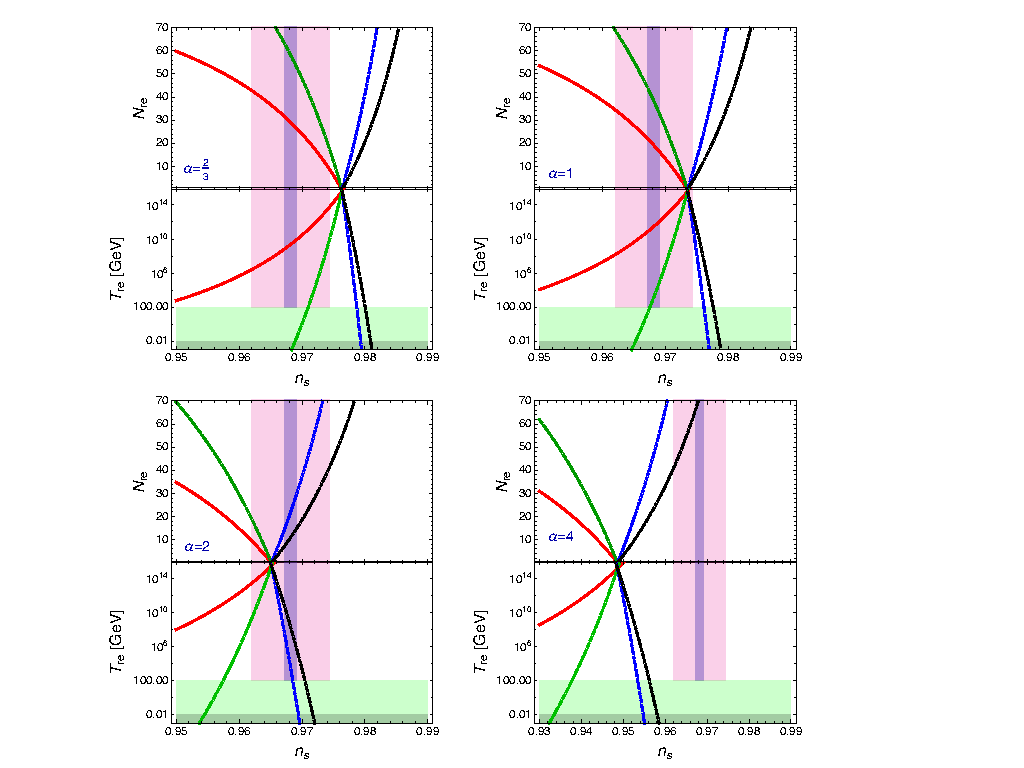
\includegraphics[width=1\linewidth, height=0.3\textheight]{Images/Chap3/Cook_Fig.2}
	\caption{Plots of $ N_{re} $ and $ T_{re} $, the length of reheating and the temperature at the end of reheating, respectively, for polynomial potentials with exponent $\alpha$. The solid red line corresponds to $ \omega_{re}=-1/3 $, the dashed green line to $\omega_{re}=0$, the dotted blue line to $ \omega_{re}=2/3 $, and the dot-dashed black line to $\omega_{re}=1$. The pink shaded region corresponds to the $ 1\sigma $ bounds on $ n_{s} $ from Planck. The purple shaded region corresponds to the $ 1\sigma $ bounds of a further CMB experiment with sensitivity $ 10^{-3} $, using the same central $ n_{s} $ value as Planck. Temperatures below the dark green shaded region are ruled out by BBN. The light green shaded region is below the electroweak scale, assumed 100 GeV for reference. This region is not disallowed but would be interesting in the context of baryogenesis \cite{Chap3:Cook}. }
	\label{fig:cookfig}
\end{figure}
 In (Fig. \ref{fig:cookfig}) from \cite{Chap3:Cook} are computed $ N_{re} $ and $ T_{re} $ as functions of $ n_{s}-1 $ for power-law potentials with $\alpha=2/3,1,2,4$. The results indicate that the quadratic potential $\alpha=2$ implies a prolonged reheating epoch for the central value $ n_{s} \simeq 0.96 $ and canonical reheating ($ \omega_{re} = 0 $). It is required a reheating temperature $ T_{re}\simeq 10^{6} $, and a number $ N_{re} \simeq 30 $ of e-folds in this case. Instead, a scalar tilt bluer than 0.96 requires smaller $ N_{re} $ and higher reheating temperature. In \cite{Chap3:Kai_Kamionkowsy}  is derived from  numerical analysis a relation between the reheat temperature $ T_{re} $ and the scalar spectral index $ n_{s} $, given by $ \log_{10}(T_{re}/10^{6}GeV) \simeq 2000(n_{s}-0.96) $. From this formula we see that an higher reheat temperature $ T_{re} $ implies a larger $ n_{s} $. If $ T_{re} $ is considerably above the electroweak scale, then $ n_{s} $ will have to be larger than its central value. For example, if reheating was nearly instantaneous and set $ T_{re}\simeq 10^{16} $ GeV, as may required by GUT-scale baryogenesis models, then quadratic inflation requires $ n_{s}\simeq 0.965 $ (taking $ k=0.05 Mpc^{-1} $ used by Planck. This value increase to $ n_{s} \simeq 0.967 $ for the WMAP pivot scale $ k=0.02 Mpc^{-1} $ ).\\
For models with smaller power-law indeces ($ \alpha=2/3,1 $), canonical reheating is too efficient in diluiting the energy density if $ n_{s} $ falls within its $ 1\sigma $ error range. These types of model (axion-monodromy models), unless $ n_{s} $ is above the current $ 1\sigma  $ upper limit, require some exotic mechanism of reheating, beyond that in the canonical scenario. On the other hand, models with larger power-law potentials indeces ($\alpha=3,4$), require $\omega_{re} > 1/3 $ (irrealistic considering that this would mean a diluition of energy density faster than that occurs during the radiation epoch). Thus, also in these models reheating  require some non-canonical picture, unless $ n_{s} $ is near the lower limit of the current $ 2\sigma $ range.\\
In conclusion, the analysis suggests that the power-law inflationary models, with $ \alpha=2 $, are the most compatible with the simplest canonical reheating scenario. The current data then do seem to favor a simple quadratic inflaton potential if a simple reheating scenario is assumed \cite{Chap3:Cook}.\\
In \cite{Chap3:Cook} is studied, with the approach discussed in this section, a broad range for the equation of state parameter, $ -1/3 \le \omega_{re} \le 1 $  with the corresponding limits on CMB observables for different inflationary models. From the analysis comes out that a $\phi^{2}$ potential would favor relatively large values of $ r $. For example, a reheating model with $ \omega_{re} \le 1 $ imples $ r\ge 0.11 $. On the other hand, to allow a reheating model with $\omega_{re} \le 1/3$, which is very probable, the tensor-to-scalar ratio requires to be $ r\ge 0.14 $. For natural inflation, considered in the previous chapter, the paper finds that  Planck's $ 2\sigma $ bound on $ n_{s} $ favors a tensor-to-scalar ratio $ r\ge 0.05 $ for $ \omega_{re} \le 1/3 $.
 \section{Bayesian approach}
 We end this chapter considering the Bayesian approach to have informations about reheating using CMB. So far, the contraints on the reheating temperature and the reheating energy scale are not so numerous. The reheating temperature should be less than $ 10^{16}  $ GeV, and also should proceed before BBN implying $ T_{reh} \ge 10 $ MeV. Thus, the reheating temperature is poorly constrained, in particular its lower limit.\\
 In \cite{Chap3:Martin_Ringeval} are derived constraints on the reheating phase, making use of Bayesian techniques and utilizing a full numerical approach. This approach has several advantages. First, the method remains accurate when the slow-roll approximation breaks down, as one expects near the end of inflation. Second, it permits a new treatment of reheating. Indeed, instead of viewing the reheating parameters as a nuisance collection of parameters, they can easily be included in the Bayesian data analysis process. Third, the evolution of cosmological perturbations in the hot big-bang theory already relies on numerical codes. Treating peerturbations during inflation in the same way allows to automatize the entire procedure and to be easily extended to other scenarios. Fourth, the numerical approach allows us to solve the problem of the prior choice. Indeed, from a physical point of view, our prior knowledge is on the inflationary theory and not the shape of the primordial power-spectra which is actually a model prediction. Therefore, it is better and easier to choose prior probability distributions directly on model parameters, such as the power index of the large-field potentials \cite{Chap3:Martin_Ringeval}.\\
 In this section we only outline the main points. For a complete treatment see \cite{Chap3:Martin_Ringeval}, where the Bayesian approach was first introduce to study reheating, \cite{Chap3:Martin_Observing_Reheating} which is based on Planck 2013 data, and \cite{Chap3:Martin_Milestone} based on Planck 2015 data (using a better analysis).\\
 \\
 The evolution of scalar density perturbation is described by the Mukhanov-Sasaki variable $ v_{k} $, seen in the first chapter (in accordance with the literature, we renamed $ \mathcal{Q}_{k} $ with $ v_{k} $ ). The equation (\ref{finalEOM}) can be rewritten in terms of the slow-roll parameter $\epsilon$:
 \begin{equation}
\label{Chap3:equationScalarPerturbations}
v_{k}'' + \Bigg[k^{2} - \frac{(a\sqrt{\epsilon})''}{a\sqrt{\epsilon}}\Bigg]v_{k}=0.
 \end{equation}
The Mukhanov-Sasaki variable $ v_{k} $ is related to the curvature pertubation $\zeta_{k}$ through the following relation
\begin{equation}
	\label{Chap3:Zetak}
	\zeta_{k} = \frac{1}{M_{pl}}\frac{v_{k}}{a\sqrt{2\epsilon}},
\end{equation}
From which we derive the power spectrum of $ \zeta_{k} $,
\begin{equation}
	\label{Chap3:PowerSpectrum}
	P_{\zeta_{k}} \equiv \frac{k^{3}}{2\pi^{2}}|\zeta_{k}|^{2}=\frac{k^{3}}{4\pi^{2}M_{pl}^{2}}\Bigg|\frac{v_{k}}{a\sqrt{\epsilon}}\Bigg|^{2}.
\end{equation}
To obtain the power sperctrum $ P_{\zeta}(k) $, one has to integrate (\ref{Chap3:equationScalarPerturbations}) with initial conditions given by the Bunch-Davis vacuum 
\begin{equation}
	\label{Chap3:BunchDavis}
	\lim_{k/\mathcal{H} \rightarrow +\infty} v_{k} = \frac{1}{\sqrt{2k}}e^{-ik\tau},
\end{equation}
since, at the beginning of inflation, all the modes of astrophysical interest today were much smaller than the Hubble radius.\\
As said in the first chapter, the curvature perturbation $\zeta_{k}$ is directly linked to CMB anisotropies and it is a conserved quantity on large scales. This means that one can use it to propagate the inflationary spectrum from the end of inflation to the post-inflationary era. In other words, the power spectrum is not affected by the post-inflationary evolution, in particular by the reheating stage. However, in the previous section we have seen that the relation between the physical scales at present and during inflation depends on the properties of the reheating epoch. Thus, in order to calibrate the inflationary spectrum with respect to the physical scales of astrophysical interest today, we need to know how reheating proceed.\\
We can express (\ref{Chap3:equationScalarPerturbations}) in terms of the number of e-folds during inflation, $ N=\ln (a/a_{in}) $, where $ a_{in} $ is the value of the scale factor at the beginning of inflation. It can be written as 
\begin{equation}
\label{Chap3:scalarPerturbation}
\frac{d^{2} v_{\textbf{k}}}{dN^{2}} + \frac{1}{\mathcal{H}}\frac{d\mathcal{H}}{dN}\frac{dv_{\textbf{k}}}{dN} + \Bigg[\Bigg(\frac{k}{\mathcal{H}}\Bigg)^{2}-U_{s}(N)\Bigg]v_{\textbf{k}}=0,
\end{equation}
where $ U_{s}(N) $ is an effective potential for the perturbations which depends on the scale factor and its derivative only. All the terms in the equation but $ k/\mathcal{H} $ are specified by the inflationary background evolution. Given  a physical scale today, say $ k/a_{now}=0.05 $ Mpc$^{-1} $, we need to express $ k/\mathcal{H} $ in terms of $ k/a_{now} $ and quantities defined during inflation. We can find then the relation
\begin{equation}
\label{Chap3:kH}
\frac{k}{\mathcal{H}}=\frac{\Gamma_{k}}{H(N)}e^{N_{T}}e^{-N},
\end{equation}
where $ N_{T} $ is the total number of e-folds during inflation. In \cite{Chap3:Martin_Ringeval} was defined $\Gamma_{k}$ as
\begin{equation}
	\label{Chap3:Gammak}
	\Gamma_{k}\equiv \frac{k}{a_{now}}(1+z_{now}) = \frac{k}{a_{now}}\Bigg(\frac{\rho_{end}}{\Omega_{\gamma}\rho_{cr}}\Bigg)^{1/4}R^{-1}_{rad},
\end{equation}
where in the paper was introduced the new parameter $ R_{rad} $. This parameter plays a crucial role in this treatment. $\rho_{end}$ is the energy density at the end of inflation, $\rho_{cr}$ is the present day critical energy density and $\Omega_{\gamma} \simeq 2.471 \times 10^{-5} h^{-2}$ is the density parameter of radiation today.
The parameter $ \Gamma_{k} $ depends on the whole post-inflationary evolution of the universe through $ z_{end} $. After inflation only the reheating phase is poorly known and represents the main source of uncertainty for the inflationary predictions.\\
In order to find the physical interpretation of $ R_{rad} $, assume that the reheating phase is dominated by a conserved effective fluid with energy density $\rho$ and pressure $ P $, with the equation of state parameter $\omega_{re}$.  We can define the energy density during reheating as
\begin{equation}
	\label{Chap3:energyDensityDuringReheating}
	\rho(N) = \rho_{end} \exp \Biggl\{-3 \int_{N_{T}}^{N}[1+\omega_{re}(n)]dn\Biggr\}.
\end{equation}
From this expression, we can derive
\begin{equation}
\label{Chap3:lnRad}
\ln R_{rad} = \frac{\Delta N}{4}(-1 + 3\bar{\omega}_{re}),
\end{equation}
where 
\begin{equation}
	\Delta N \equiv N_{re} - N_{T}
\end{equation}
is the total number of e-folds during reheating, being $ N_{re} $ the number of e-folds at which reheating is completed and the radiation dominated era begins. The parameter $\bar{\omega}_{re}$ denotes the mean equation of state parameter
\begin{equation}
\label{Chap3:meanEqStateParametere}
\bar{\omega}_{re}\equiv \frac{1}{\Delta N}\int_{N_{T}}^{N_{re}}\omega_{re}(n)dn.
\end{equation}
Then the parameter $ R_{rad} $  only depends on what happens during reheating. In the special case  in which $ \bar{\omega}_{re}=1/3 $, $ \ln R_{rad}=0 $ and, in this case, the reheating stage cannot be distinguished from the subsequent radiation dominated era and cannot affect the inflationary predictions. This also implies $ R_{rad}=1 $.\\
From (\ref{Chap3:energyDensityDuringReheating}), $ \ln R_{rad} $ can be put in the form
\begin{equation}
\label{Chap3:Rrad2}
\ln R_{rad}= \frac{1-3\bar{\omega}_{re}}{12(1+\bar{\omega}_{re})}\ln \Bigg ( \frac{\rho_{re}}{\rho_{end}} \Bigg)
\end{equation}
where $ \rho_{re} $ is the energy density at the end of the reheating era. \\
 We can summarise the discussion. In order to calculate the power spectrum of the inflationary cosmological perturbations, we need to solve (\ref{Chap3:scalarPerturbation}). In this formula the only term not known during inflation is $ k/\mathcal{H} $, which depends on the parameter $ R_{rad} $ that is the only parameter that contains informations about the reheating stage. More precisely, it depends on the energy density at the end of reheating, $\rho_{re}$, and on the mean equation of state $\bar{\omega}_{re}$.\\
 Having discussed the phisical interpretation of $ R_{rad} $, we can explain how it is constrained from CMB observations. $ R_{rad} $ can be expressed in terms of quantities defined at the Hubble horizon crossing,
 \begin{equation}
 	\label{Chap3:RradHorizonCrossing}
 	\ln R_{rad} = N_{T} - N_{*} + N_{0} - \frac{1}{4}\ln \Bigg(\frac{H_{*}^{2}}{M_{pl}^{2}\epsilon_{*}}\Bigg) +\frac{1}{4}\Bigg(\frac{3}{\epsilon_{*}}\frac{V_{end}}{V_{*}}\frac{3-\epsilon_{*}}{3-\epsilon_{end}}\Bigg),
 \end{equation}
 where it is defined
 \begin{equation}
\label{Chap3:reheatingN0}
N_{0} \equiv \ln \Bigg(\frac{k/a_{now}}{\rho_{\gamma}^{1/4}}\Bigg).
 \end{equation}
 In (\ref{Chap3:RradHorizonCrossing}),  $ N_{*} $ is the e-folds number at which the scale $ k/a_{now} $ crossed out the Hubble radius during inflation and same thing for the other quantities. In order to be consistent with the standard cosmological model, $ \ln R_{rad} $ cannot take any arbitrary values. One shoud have $\bar{\omega}_{re}<1$ to respect the positivity energy conditions of General Relativity, and $ \bar{\omega}_{re} > -1/3 $ by the fact that reheating is not inflation. Moreover, reheating should occur after inflation and before BBN, i.e. $\rho_{nuc} < \rho_{re} < \rho_{end}$, with
 \begin{equation}
 	\label{Chap3:rhoNuc}
 	\rho_{nuc}\equiv(10^{4}MeV)^{4}
 \end{equation} 
From this we can directly explicitily (\ref{Chap3:RradHorizonCrossing}) (see \cite{Chap3:Martin_Ringeval}).\\
The equation (\ref{Chap3:RradHorizonCrossing}) can be used in two manners. The first way is to assume something about $ R_{rad} $ and derive the corresponding range of variations of the slow-roll predictions $ N_{*} $ and $\epsilon(N_{*})$. In other words, this determines how the inflationary predictions depend on the details of the reheating era. This approach is the mostly used in the literature to compare inflationary predictions to the current contraints on the slow-roll parameters $\epsilon_{*}$ (or spectral index and tensor-to-scalar ratio). But, as pointed out in the paper, this is made by choosing a value of $ N_{*} $, which is directly linked to $ R_{rad} $, which itself depends on the energy density at which reheating ends, and on the equation of state during reheating. The range of variation for $ N_{*} $ then can only be known once a reheating model is assumed. Without such assumption, an assumed value of $ N_{*} $ can cause inconsistencies with standard cosmology (for example reheating occurring after BBN, or at energy densities higher than $\rho_{end}$).\\
The second approach, introduced in the \cite{Chap3:Martin_Ringeval}, consists of considering $ R_{rad} $ as an observable model parameter and includying it in the data analysis using a Bayesian approach. If we have specified a model, and then a potential, $ V_{end} $ is explicitily known. CMB data put a limit on $ H_{*}^{2}/\epsilon_{*} $, through the amplitude of the anisotropies, as well as on $\epsilon_{*}$ from the tensor-to-scalar ratio. One can expects CMB data to also give some informations on $ R_{rad} $. Therefore, to discuss how well CMB data constraint a set of inflationary models is to perform a Bayesian analysis of the data given the model parameters, including reheating. This is different than constraining the slow-roll parameters, or the spectral index and the tensor-to-scalar ratio, which only encode the shape of the primordial power spectra and know nothing about reheating (while a model of inflation does). The numerical exact integration method consists of the computation of the primordial power spectra assuming only General Relativity and linear perturbation theory. Therefore the only model parameters are the ones appearing in the inflaton potential together with the reheating parameters $ R_{rad} $. In \cite{Chap3:Martin_Ringeval} is performed data analysis for both  large and small field models. It is showed that CMB data restrict the \textit{a priori} possible values of $ \Delta N $ and $\bar{\omega}_{re}$\\
In \cite{Chap3:Martin_Observing_Reheating} and \cite{Chap3:Martin_Milestone} the analysis are computed with the Planck data. In these papers are derived the posterior probabilities of the reheating parameters associated with almost 200 inflationary models taken from \textit{Encyclopedia Inflationaris} \cite{Chap3:EncyclopediaInflationaris}. Such a number is representative of all the single-field slow-roll models proposed (until 2015). This analysis allows to obtain  generic conclusions and new constraints on the inflationary reheating within the slow-roll.\\
 Performing a CMB data analysis within one model of inflation allows one to infer, among others, the marginalized posterior probability distribution $ P(\ln R_{re}|D
) $ for the parameter $ R_{re} $ defined as $R_{re}=R_{rad}\ (\rho_{end}^{1/4}/M_{pl})  $, under the dataset D.  Considering that reheating should occur after inflation and before BBN, and the conditions seen on the equation of state parameter $ -1/3 < \bar{\omega}_{re} < 1 $, one derives
\begin{equation}
	\label{Chap3:PriorChoiche}
	-46 < \ln R_{reh} < 15 + \frac{1}{3}\ln\Bigg( \frac{\rho_{end}}{M_{pl}^{4}}\Bigg).
\end{equation}
These bounds define a flat prior probability distribution $ \pi(\ln R_{reh}) $. The data are constraining the reheating epoch as soon as the posterior P is peaked compared to the prior $\pi$. Since the simple ratio of standard deviations wastes some information, in \cite{Chap3:Martin_Milestone}  is used the Kullback-Leibler divergence between the prior distribution $\pi$ and the posterior P,
\begin{equation}
\label{Chap3:KullbackLeiblerDivergence}
D_{KL}=\int P(\ln R_{reh}|D)\ln \Bigg[\frac{P(\ln R_{reh})}{\pi(\ln R_{reh})}\Bigg]d \ln R_{reh}
\end{equation}
which is a measure of the amount of information provided by the data D about $ \ln R_{reh} $.
In order to perform the CMB data analysis of the almost 200 slow-roll inflationary models, \cite{Chap3:Martin_Milestone} considered an effective likelihood $\mathcal{L}_{eff}$ depending  only by the slow-roll parameters ($ P_{*},\epsilon_{i*} $). This likelihood is obtained by marginalitation of the joint Planck 2015 and BICEP2/KECK likelihood over all the other parameters $ \theta_{iac} $ that corresponds to the instrumental, astrophysical and cosmological parameters.\\
The effective likelihood is defined as 
\begin{equation}
\label{Chap3:effectiveLikelihood}
\mathcal{L}_{eff}(P_{*},\epsilon_{i*}) \equiv \int P(D|\theta_{iac}, P_{*}, \epsilon_{i*})\pi(\theta_{iac})d\theta_{iac}.
\end{equation} 
Within a given slow-roll model of inflation $\mathcal{M}$, with theoretical parameters $\theta_{inf}$, the quantities $ P_{*} $ and $ \epsilon_{i*} $ are explicit function of $\theta_{inf}$ and, most importantly of $ \ln R_{reh} $. Thus, from Bayes' theorem, the posterior on $ \ln R_{reh} $ is given by
\begin{equation}
	P(\ln R_{reh}|D)= \frac{\pi(ln R_{reh})}{P(D|M)}
	\times \int \mathcal{L}[P_{*}(\theta_{inf},\ln R_{reh}), \epsilon_{i*}(\theta_{inf},\ln R_{reh})]\pi(\theta_{inf})d\theta_{inf},
\end{equation}
where $ P(D|M) $ is the global likelihood, which is proportional  to the Bayesian evidence $ P(\mathcal{M}|D)=P(D|\mathcal{M})\pi(\mathcal{M}) $ of the model $\mathcal{M}$ to explain the data D.\\
To fix better the idea in (Fig. \ref{fig:martinfig2a}) is reported the plot of \cite{Chap3:Martin_Milestone}, in which are represented the posteriors of $ \ln R_{reh} $ for two particular models: loop inflation and supergravity brane inflation using both the Planck 2013 and 2015 data. From the figure we can see the gain of information between these two data sets as well as the overall constraining power of CMB data on reheating. Of course, for other models $ \mathcal{M}_{i} $, the posteriors on $ \ln R_{reh} $ are different and may be peaked over large or small values, or not constrained at all.\\
We show in (Fig. \ref{fig:martinfig3a}) also the main plot of \cite{Chap3:Martin_Milestone}. In the plot each model is represented by a circle in the plane ($ \mathcal{B},D_{KL} $) where $\mathcal{B}$ is the Bayes' factor normalized to the best model, obtained from the global likelihoods by 
\begin{equation}
	\label{Chap3:BayesFactor}
	\mathcal{B} \equiv \frac{P(\mathcal{M}_{i}|D)}{sup_{j}[P(M_{j}|D)]}.
\end{equation}
Most of the models having large Bayes factor are concentrated around values $ D_{KL} \le 1 $, whereas disfavored models have $ D_{KL} > 2.5 $. This indicates how good a model fits the data. In the paper it is calculated also the average value of $ D_{KL} $ in the space of all models for Planck 2013 and Planck 2015 data, with 
\begin{equation}
<D_{KL}>\sum_{i} P(\mathcal{M}_{i}|D)D_{KL}(\mathcal{M}_{i}).
\end{equation}
This value is weighted by the Bayesian evidence, namely the probability of a model to explain the data. Disfavored models weight less than favored models. The authors estimate $ <D_{KL}> = 0.82 \pm 0.26 $ for Planck 2015 and  $ <D_{KL}> = 0.55 \pm 0.14 $. This leads a $ 40\% $ improvement in information gain from Planck 2015 compared to Planck 2013.
\begin{figure}
	\centering
	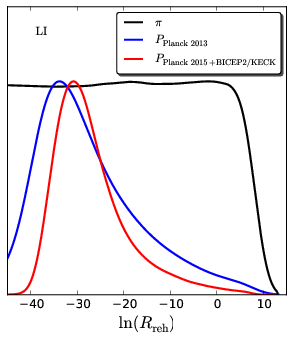
\includegraphics[width=0.45\linewidth, height=0.3\textheight]{Images/Chap3/Martin_Fig2A}
	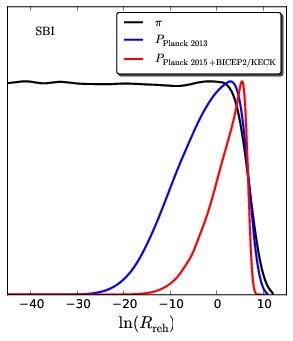
\includegraphics[width=0.45\linewidth, height=0.3\textheight]{Images/Chap3/Martin_Fig2B}
	\caption{Probability distributions (normalized to their maximum) for the rescaled reheating parameter $ R_{reh} $ associated with two of the 200 models analyzed: loop inflation on the left (LI) and supergravity brane inflation on the right (SBI) [\cite{Chap3:BraneInflation}]. The black curve corresponds to the prior (\ref{Chap3:PriorChoiche}) and is not exactly flat since the upper bound of (\ref{Chap3:PriorChoiche}) is slightly model dependent. The marginalized posterior obtained from  Planck 2013 data is displayed in blue and is to be compared to the more constraining posterior obtained from the Planck 2015 with BICEP/KECK (red curve) \cite{Chap3:Martin_Milestone}.}
	\label{fig:martinfig2a}
\end{figure}
\begin{figure}[h]
	\centering
	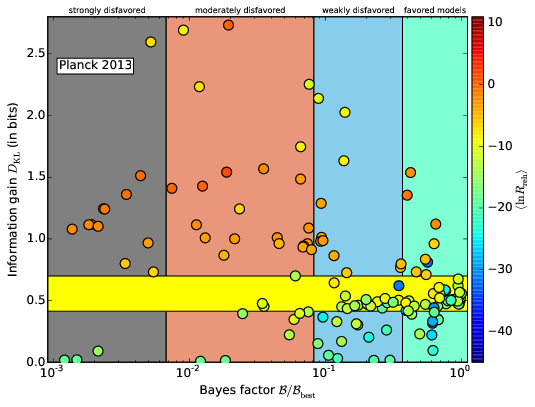
\includegraphics[width=0.75\linewidth, height=0.3\textheight]{Images/Chap3/Martin_Fig3A}
	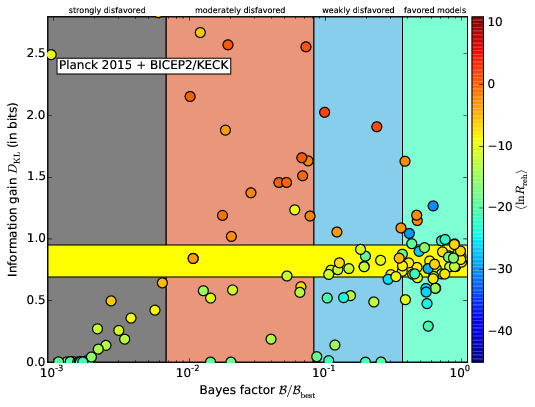
\includegraphics[width=0.75\linewidth, height=0.3\textheight]{Images/Chap3/Martin_Fig3B}
	\caption{Information gain $ D_{KL} $ in (bits) given by Planck 2013 (left panel) and Planck 2015 with BICEP2/KECK (right panel) about the rescaled reheating parameter $ \ln R_{reh} $ as a function of the Bayesian evidence. Each circle represents one of the 200 models of the \textit{Encyclopedia Inflationaris} collection whose color traces the mean value of $ \ln R_{reh} $. The yellow band represents the one-sigma deviation around the mean value. For Planck 2015 and BICEP2/KECK, one gets $ <D_{KL}> = 0.82 \pm 0.13 $. This corresponds to $ 40\% $ improvement compared to Planck 2013 \cite{Chap3:Martin_Milestone}. } 
	\label{fig:martinfig3a}
\end{figure}
\chapter{Preheating}

\chapter{Other models of Preheating}

\chapter{Non Linear Evolution After Preheating: Bubbly Stage}

\chapter{Thermalitation}


\chapter{Other Signatures of Reheating}

\begin{thebibliography}{2}
	
	\bibitem{Liddle:intro} A. R. Liddle and D. H. Lyth, \emph{Cosmological inflation and large-scale structure} (Cambridge University Press, 2006).
	
	\bibitem{NonGauss:Intro} N. Bartolo, E. Komatsu, S. Matarrese and A. Riotto, Phys. Rept. \textbf{402}, 103 (2004) [arXiv:astro-ph/0406398].
	
	\bibitem{GWFromInflation:Intro} M. C. Guzzetti, N. Bartolo, M. Liguori and S. Matarrese, (2016), arXiv:1605.01615. 
	
	\bibitem{Guth:Intro} A. Guth, Phys. Rev. \textbf{D23}, 347 (1981) .
	
	\bibitem{COBE1:intro} K. M. G´orski, et al. Astrophys. J. \textbf{464}, L11 (1996) [arXiv:astro-ph/9701191].
	
	\bibitem{COBE2:intro} G. F. Smoot, et al., Astrophys. J. \textbf{396}, L1 (1992).

    \bibitem{WMAP:intro} H. V. Peiris, et al., Astrophys. J. Suppl. \textbf{148}, 213 (2003).
	
	\bibitem{Planck2018:intro} Y. Akrami et al., Astron. Astrophys. \textbf{641}, A9 (2020).
	
	\bibitem{Steigman:nucleosynthesisIntro} G. Steigman, Ann.Rev.Nucl.Part.Sci. \textbf{57}, 463-491 (2007) [arXiv:0712.1100].
	
	\bibitem{ReheatingPredictionsSingleFieldModel:intro} J.L. Cook et al., JCAP \textbf{1504} (2015) 047 [arXiv:1502.04673].
	
	\bibitem{Bicep2:Intro} BICEP2, Keck Array, P.A.R. Ade et al., Phys. Rev. Lett. \textbf{116}, 031302 (2016) [arXiv:1510.09217].
	
	\bibitem{Bicep2BMode:Intro} BICEP2 Collaboration, P. Ade et al., Phys. Rev. Lett. \textbf{112} (2014) 241101 [arXiv:1403.3985].
	
	\bibitem{COre:intro} COrE, F. R. Bouchet et al., (2011), arXiv:1102.2181.  
	
	\bibitem{PRISM:intro} PRISM, P. Andrè et al., JCAP \textbf{1402}, 006 (2014) [arXiv:1310.1554].
	
	\bibitem{LIGO:intro} LIGO Scientific, J.Aasi et al., Class. Quant. Grav. \textbf{32} (2015) 074001 [arXiv:1411.4547].
	
	\bibitem{Lisa:Intro} A. Klein et al., Phys. Rev. \textbf{D93}, 024003 (2016) [arXiv:1511.05581].
	
	\bibitem{InflationDynamicsAndReheating:chap1} B. A. Bassett, S. Tsujikawa and D. Wands, Rev. Mod. Phys. \textbf{78}, 537 (2006) [arXiv:astro-ph/0507632].
	
	\bibitem{Dodelson:Chap1} S. Dodelson, F. Schmidt, \emph{Modern Cosmology} (Academic Press, 2020).
	
	\bibitem{TopDefects:Linde} A. Linde,  (1990), arXiv:hep-th/0503203.
	
	\bibitem{Plank2015:Chap1} Planck, P. A. R. Ade et al., (2015), arXiv:1502.02114.
	
	\bibitem{Chap2:Fig1} A. Albrecht, (2000), arXiv:astro-ph/0007247.
	
	\bibitem{Chap2: Linde_NewInflation} A. D. Linde, Phys. Lett. \textbf{B108}, 389 (1982).
	
	\bibitem{ChaoticInflationLinde:Chap2} A. D. Linde, Phys. Lett. \textbf{B129}, 177  (1983).  
	
	\bibitem{Chap2:Linde_HystoryInflation} A. Linde, (2007), arXiv: 0705.0164. 
	
	\bibitem{Chap2:NaturalInflation} K. Freese, J. A. Frieman and A. V. Olinto, Phys. Rev. Lett. \textbf{65}, 3233 (1990).
	
	\bibitem{Chap2:NaturalInflation_Turner_Steinhardt} P. J. Steinhardt and M. S. Turner, Phys. Rev. \textbf{D29}, 2162 (1984).
	
	\bibitem{Chap2:AxionModel} J. E. Kim, Phys. Rep. \textbf{150}, 1 (1987).
	
	\bibitem{Chap2: Hybrid_Model} A. Linde, (1993), arXiv: astro-ph/9307002.
	
	\bibitem{Chap2:PerturbationsHybridInflation} J. Garcìa-Bellido, A. D. Linde and D. Wands, Phys. Rev. \textbf{D54}, 377 (1996).
	
	\bibitem{Chap2:Planck2018} Planck Collaboration, Astron. Astrophys. \textbf{641}, A10 (2020).
	
	\bibitem{Chap2:Wilkinson} H. V. Peiris \textit{et al.}, Astrophys. J. Suppl. \textbf{148}, 213 (2003) [arXiv:astro-ph/0302225].
	
	\bibitem{Chap2:Kolb_Turner} E. W. Kolb, M. S. Turner, \textit{The Early Universe} (Westview Press, 1994).
	
	\bibitem{Chap3:GW_Watanabe_Komatsu} Y. Watanabe, E. Komatsu, Phys. Rev. \textbf{D73}, 123515 (2006) [arXiv:astro-ph/0604176]
	
	\bibitem{Chap3:GW_Turner_White} M. S. Turner, M. White and J. E. Lidsey, Phys. Rev. \textbf{D48}, 4163 (1993).
	
	\bibitem{Chap3: Gravitation} C. W. Misner, K. S. Thorne and J. A. Wheeler, \textit{Gravitation} (Princeton Univ Pr, 2017).
	
	\bibitem{Chap3:Kamionkowsy_Turner} M. Kamionkowsy, A. Kosowsky and M. S. Turner, Phys. Rev. \textbf{D49}, 2837 (1994).
	
	\bibitem{Chap3:ProibingReheatingTemperature2008} K. Nakayama, S. Saito, Y. Suwa and J. Yokoyama, JCAP 0806, 020 (2008) [arXiv:0804.1827].
	
	\bibitem{Chap3:ProspectsForDeterminationWithDetectors} S. Kuroyanagi, K. Nakayama and S. Saito, Phys. Rev. \textbf{D84}, 123513 (2011) [arXiv:1110.4169].
	
	\bibitem{Chap3:BlueTiltedSpectrum} S. Kuroyanagi, T. Takahashi and S. Yokoyama, JCAP 1502, 003 (2015) [arXiv:1407.4785]. 
	
	\bibitem{Chap3: DECIGO} N. Seto, S. Kawamura and T. Nakamura, Phys. Rev. Lett. \textbf{87}, 221103 (2001).
	
	\bibitem{Chap3:Seto_Yokohama} N. Seto and J. Yokoyama, J. Phys. Soc. Jap. \textbf{72}, 3082 (2003).
	
	\bibitem{Chap3:Ligo_Virgo} J. Aasi \textit{et al.} [LIGO Scientific and VIRGO Collaborations], arXiv:1406.4556 [gr-qc].
	
	\bibitem{Chap3:PulsarTiming} P. B. Demorest, R. D. Ferdman, M. E. Gonzalez, D. Nice, S. Ransom, I. H. Stairs, Z. Arzoumanian and A. Brazier \textit{et al.}, Astrophys. J. \textbf{762}, 94 (2013) [arXiv:1201.6641].
		
	\bibitem{Chap3:BBN} M. Maggiore, Phys. Rept. \textbf{331}, 283 (2000) [arXiv:gr-qc/9909001].	
	
	\bibitem{Chap3:Podolsky_Felder} D. I. Podolsky, G. N. Felder, L. Kofman and M. Peloso, Phys. Rev. \textbf{D73}, 023501 (2006) [arXiv:hep-ph/0507096].
	
	\bibitem{Chap3:Cook} J. L. Cook \textit{et al.}, JCAP 1504, 047 (2015) [arXiv:1502.04673].
	
	\bibitem{Chap3:Kai_Kamionkowsy} L. Dai, M. Kamionkowski and J. Wang, Phys. Rev. Lett. \textbf{113}, 041302 (2014) [arXiv:1404.6704].
	
	\bibitem{Chap3:Martin_Ringeval} J. Martin and C. Ringeval, Phys. Rev. \textbf{D82}, 023511 (2010) [arXiv:1004.5525].
	
	\bibitem{Chap3:Martin_Observing_Reheating} J. Martin, C. Ringeval and V. Vennin, Phys. Rev. Lett. 114, 081303 (2015). [arXiv:1410.7958].
	
	\bibitem{Chap3:Martin_Milestone} J. Martin, C. Ringeval and V. Vennin, Phys. Rev. \textbf{D93} 10, 103532 (2016) [arXiv:1603.02606].
	
	\bibitem{Chap3:EncyclopediaInflationaris} J. Martin, C. Ringeval, R. Trotta and V. Vennin, JCAP \textbf{1403}, 039 (2014) [arXiv:1312.3529].
	
	\bibitem{Chap3:BraneInflation} J. Martin, C. Ringeval and V. Vennin, Phys. Dark Univ. \textbf{5-6}, 75 (2014) [arXiv:1303.3787].
		
\end{thebibliography}	
	
\end{document}
